\documentclass[master]{thesis-uestc}
\usepackage{tikz} % 必须的基础绘图包


% 此处-----------|---的模板类型设置请参照README
\title{大功率宽频带脊波导微波窗研究}{Research on High-Power Broadband Ridge Waveguide Microwave Window} % 论文题目
\author{方源}{Fang Yuan} % 作者姓名
\setdate[submit]{ } % 论文提交日期,可留空
\setdate[oral]{ }  % 答辩日期,可留空
\setdate[confer]{ } % 学位授予日期,可留空
\advisor{\qquad 王建勋\qquad\qquad 教\chinesespace 授}{Wang Jianxun Prof.}
% \coAdvisor{合作导师姓名\chinesespace 导师职称}{Co advisor English name English title} % 仅专业硕士/博士使用,在扉页/英文首页添加合作导师,不使用请注释
\school{电子科学与工程学院}{School of Electronic Science and Engineering} % 学院信息
\major{电子科学与技术}{Electronic Science and Technology} % 专业信息
\studentnumber{202221020122} % 学号
\ProfessionalDegreeArea{随便学学} % 专业硕士专用:专业学位领域
\ClassificationNumber{TP309.2} % 分类号
\ClassifiedClass{公开} % 密级
\UDCNumber{004.78} % UDC号
\Chairman{xxxxx} % 答辩委员会主席

% 取消注释以下内容,用于禁止文中换行处的英语单词自动截断换行。
% \tolerance=1
% \emergencystretch=\maxdimen
% \hyphenpenalty=10000
% \hbadness=10000

\makeglossaries % 产生缩略词表/符号表专用,不使用时请注释。 注意,之后的acronym,glossaryentry以及相关的引用也请注释。
\newacronym[description=逻辑卷管理器]{lvm}{LVM}{Logical Volume Manager} % 定义缩略词:以本项为例,逻辑卷管理器为中文名称;lvm用于文内引用;LVM为显示的应为缩略语或符号;Logical Volume Manager为显示的英文全称/描述。
\newglossaryentry{tree}{name={tree}, description={trees are the better humans}}  % 定义符号:以本项为例,name={tree}为符号名称;tree用于文内引用; description={trees are the better humans}为显示的描述。页码自动添加。

\begin{document}

\makecover % 封面+中英文扉页
\originalitydeclaration % 原创新声明
% \signatureofdeclaration{signature.pdf} % 用于添加扫描版签字后的原创新声明(使用时取消注释本行,并注释掉上一行)
% 中文摘要
\begin{chineseabstract}
    真空管在高频大功率微波系统中作为振荡器与放大器至关重要,其微波窗需拥有宽频带匹配与高气密性的特点。本文围绕宽频带紧凑型微波窗设计,开展了 6-11GHz、L 频段脊波导窗仿真设计及 W 频段窗测试与误差分析,主要内容如下:

    1. 采用双脊波导与圆柱形窗片结构,实现 6-11GHz 频段内反射系数(\(S_{11}\))<-20dB。参数分析表明过渡段厚度\(t_{rh}\)容许偏差 0.47mm,功率容量通过最大场强法(3.1kW)与二次电子倍增法(14.8kW)验证。多物理场分析显示,5kW 功率下窗片温差 11℃(<126℃安全极限),热应力低于蓝宝石抗弯强度,热变形对性能无显著影响。优化后的阶梯过渡段与标准波导 WR112 匹配良好,全频段反射系数满足测试要求。

    2. 仿真设计了L频段的宽频带脊波导窗。针对L频段应用需求,设计了一种宽频带脊波导窗。基于6-11GHz脊波导圆窗的设计基础,将窗片形状改进为圆角矩形柱状,其余结构仍采用双脊波导形式。通过最大场强法和二次电子倍增法计算,确定窗片功率容量分别为85kW和1.18kW,后者为优选值。
    针对L频段窗开展多物理场分析,在1kW功率输入下,配合空气强对流冷却,窗片温差仅为0.24℃,远低于安全极限值,顺利通过温差检验。窗片最大应力为3.76MPa,远低于BeO陶瓷的抗弯强度,因此不会因热应力导致破裂。

    3. 对W频段的窗进行了测试与误差分析。为评估W频段窗的旋转误差影响,将反射系数最优时的窗片旋转角度设为0°,并定义窗片中心竖直线为x轴。使用高度规对窗片四周每隔45°选取的点进行测量,记录这些点相对于窗片圆心的z轴高度误差。基于上述数据,建立窗片旋转状态的数学模型。计算窗片在指定旋转角度下的理论高度差,采用最小二乘法拟合实际旋转情况。拟合结果显示,旋转轴偏离窗片中心1.49mm,与x轴夹角为0.52rad,窗片旋转角度为0.0037rad,表明旋转误差极小。根据拟合结果建模发现,当窗片旋转至90°时,反射系数匹配效果最差,与实验趋势一致。研究表明,焊接加工中的旋转误差会显著影响窗片性能,这为未来工艺改进提供了重要指导。

    \chinesekeyword{L频段,微波窗,宽频带,脊波导,真空管} % 中文关键词
\end{chineseabstract}
% 英文摘要
\begin{englishabstract}
    Vacuum tubes are of critical importance in high-frequency and high-power microwave systems as oscillators and amplifiers. The microwave windows of vacuum tubes need to possess the characteristics of wide - band matching and high airtightness. This thesis focuses on the design of wide - band compact microwave windows and carries out the simulation design of ridge waveguide windows in the 6 - 11GHz and L frequency bands, as well as the testing and error analysis of W - band windows. The main contents are as follows:

1. A structure with double - ridge waveguides and cylindrical window sheets is adopted, achieving a reflection coefficient (\(S_{11}\)) < - 20dB in the 6 - 11GHz frequency band. Parameter analysis shows that the allowable deviation of the transition section thickness \(t_{rh}\) is 0.47mm. The power capacity is verified by the maximum electric field strength method (3.1kW) and the secondary electron multiplication method (14.8kW). Multiphysics analysis indicates that under a power of 5kW and with air strong convection cooling for the casing, the temperature difference of the window sheet is only 11℃ (less than the safety limit of 126℃). The thermal stress is lower than the flexural strength of sapphire, and thermal deformation has no significant impact on performance. The optimized stepped transition section matches well with the standard waveguide WR112, and the reflection coefficient across the entire frequency band meets the testing requirements.

2. A wide - band ridge waveguide window for the L frequency band is designed through simulation. Aiming at the application requirements of the L frequency band, a wide - band ridge waveguide window is designed. Based on the design of the 6 - 11GHz ridge waveguide circular window, the shape of the window sheet is improved to a rounded rectangular column, while the rest of the structure still adopts the double - ridge waveguide form. Through calculations by the maximum electric field strength method and the secondary electron multiplication method, the power capacities of the window sheet are determined to be 85kW and 1.18kW respectively, with the latter being the preferred value.
For the L - band window, multiphysics analysis is carried out. Under an input power of 1kW and with air strong convection cooling, the temperature difference of the window sheet is only 0.24℃, far lower than the safety limit, and it successfully passes the temperature difference test. The maximum stress of the window sheet is 3.76MPa, far lower than the flexural strength of BeO ceramics, so it will not break due to thermal stress.

3. Testing and error analysis of the W - band window are conducted. To evaluate the influence of the rotation error of the W - band window, the rotation angle of the window sheet when the reflection coefficient is optimal is set as 0°, and the central vertical line of the window sheet is defined as the x - axis. A height gauge is used to measure points selected every 45° around the window sheet, and the z - axis height errors of these points relative to the center of the window sheet are recorded. Based on the above data, a mathematical model of the rotation state of the window sheet is established. The theoretical height differences of the window sheet at specified rotation angles are calculated, and the least - squares method is used to fit the actual rotation situation. The fitting results show that the rotation axis deviates from the center of the window sheet by 1.49mm, the angle with the x - axis is 0.52rad, and the rotation angle of the window sheet is 0.0037rad, indicating extremely small rotation errors. Modeling according to the fitting results reveals that when the window sheet is rotated to 90°, the matching effect of the reflection coefficient is the worst, which is consistent with the experimental trend. The research shows that the rotation error in welding processing will significantly affect the performance of the window sheet, providing important guidance for future process improvements.

\englishkeyword{L-band, Microwave window, Broadband,Ridge waveguide, Vacuum tube} % 英文关键词
\end{englishabstract}

\thesistableofcontents % 目录
% \thesisfigurelist % 图目录,仅在需要时添加,一般情况下请注释
% \thesistablelist % 表目录,仅在需要时添加,一般情况下请注释
% \glsaddall % 默认仅显示被正文引用的项,取消注释以显示所有已定义的缩略词/符号
% \thesisglossarylist % 缩略词表,仅在需要时添加,一般情况下请注释
% \thesissymbollist % 符号表,仅在需要时添加,一般情况下请注释

% 正文内容


\chapter{绪\hspace{6pt}论}
\section{真空器件的发展历程}
继Fleming 在1904年发明了世界上第一只电子管——检波二极管之后不久,1906年德国科学家Forest就发明了世界上第一只三极管。从此,人类便能达到利用电子在真空中的运动这一现象,进而达到放大信号这一目的\citing{wang_microwave_2014}。随着时代的发展,人们希望将产生的电磁波的频率拔高,进而能够传输更多的信息,微波电子管便能在达到这一目的上发挥不可或缺的作用。

在常见的微波通信系统中不可或缺的一环便是放大器,常见的放大器解决方案可以被分为两个大类,一部分是基于真空电子器件的微波电子管放大器,另外一种是基于固态电子器件的放大器。根据图片\ref{fig:真空电子器件与固态电子器件的主要应用范围}中的信息可以看到\citing{kumar_2016_review},真空器件与固态器件在不同频段与功率中的适用范围。
\begin{figure}[!htb]
    \centering
    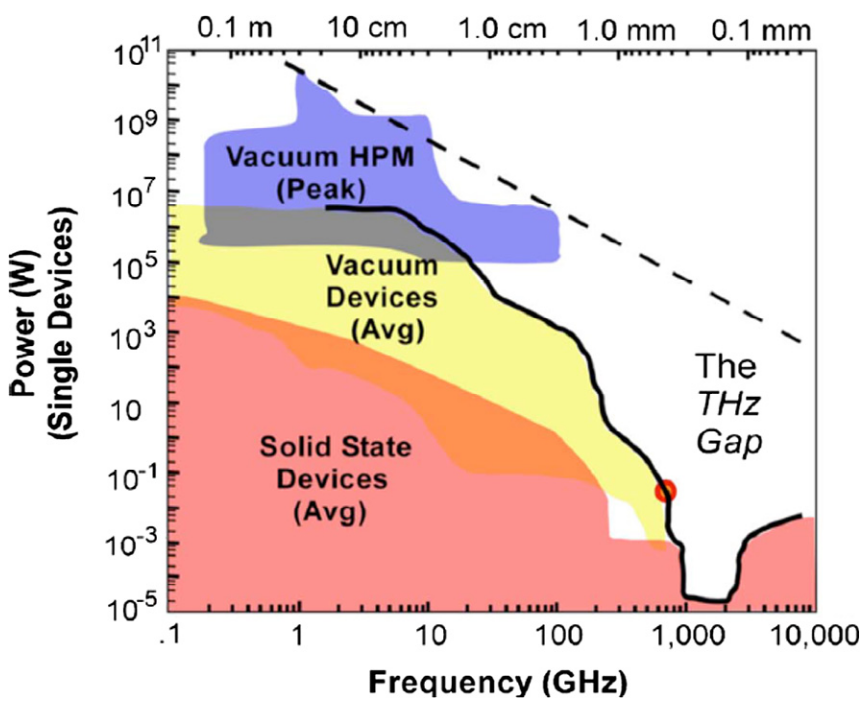
\includegraphics[width=0.5\textwidth]{pic/chapter1/器件平均功率-频率示意图.png}
    \caption{真空电子器件与固态电子器件的主要应用范围\citing{kumar_2016_review}}
    \label{fig:真空电子器件与固态电子器件的主要应用范围}
\end{figure}

根据图 \ref{fig:真空电子器件与固态电子器件的主要应用范围} 的信息,在低功率应用场合下,固态器件由于其体积较小而成为一个不错的选项。然而,在毫米波频段以上,固态器件的设计由于功率损耗和晶体管技术物理限制的影响,其进一步的应用变得极具挑战性。相比之下,在毫米波频段以上的真空器件所具备的高平均功率和高效率特性则显得尤为重要。


\section{宽带宽波导窗实现方案概述}
当真空管在地球大气内应用时,如何将能量从真空管内部真空环境传递到外界大气环境中是一个待解决的问题\citing{jr_klystrons_2011}。此时,微波窗充当了真空器件与外界大气之间的连接桥梁,具有两个主要功能:首先,它将器件内部的真空环境与外部大气隔离;其次,无论是从真空管内部传输出去还是从外界传入真空管内部,在所需的频段和功率容量范围内,以最小的反射和损耗传输信号。

微波窗是真空器件的重要组成部分之一,并且其匹配频段直接影响到真空器件的输出。现有的扩充匹配频段的方案主要作用在窗片的材料选择和形状结构,以及匹配段的形状结构之上。常见的微波窗宽带匹配方案大致上可以被分为三种可以被概述为渐变过渡匹配窗、布儒斯特窗和多层匹配窗。

在论文\cite{cook_broadband_2013_gradually}中,如图\ref{fig:渐变过渡匹配窗}所示,作者使用渐变段实现了从矩形波导的$TE_{10}$到圆波导的$TE_{11}$模式的渐变过渡,使得窗片的匹配带宽得到增宽。经过作者的调整,实现了材料为氧化铍(beryllium oxide, BeO)的窗片,在212-225GHz 的范围内达到$S_{11}<-20dB$的匹配程度。渐变过渡的优点是较为容易进行设计,并且只要确定前后段的形状后,便能使用诸如小反射理论等理论对窗片的渐变过渡段的形状进行设计指导。但是缺点是为了实现这种渐变的过渡段,需要适当的牺牲微波窗的紧凑性。微波窗的匹配部分在纵向长度上来说显得较为冗长。
\begin{figure}[!htb]
    \centering
    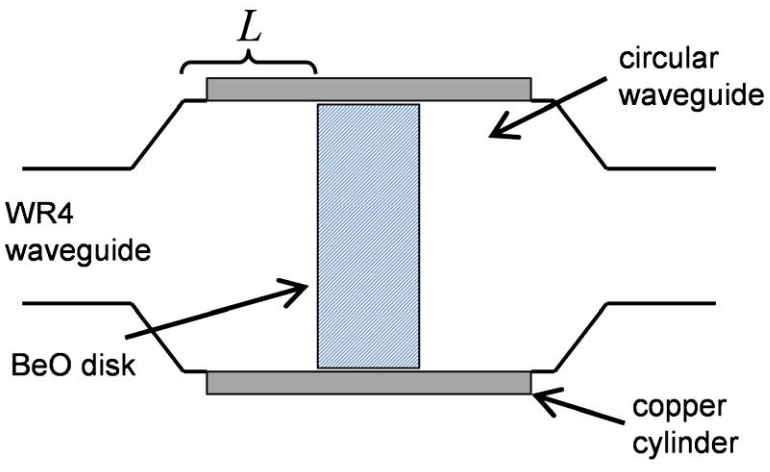
\includegraphics[width=0.5\textwidth]{pic/chapter1/渐变过渡方案.png}
    \caption{渐变过渡匹配窗\citing{cook_broadband_2013_gradually}}
    \label{fig:渐变过渡匹配窗}
\end{figure}

另外一个解决方案是多层匹配窗,多层匹配窗是一个较为宽泛的解决方案。其中包含了如图\ref{fig:宽带多层匹配窗的常见设计方案} (a)的窗片使用多种不同相对介电常数堆叠的方案\citing{wang_broadband_window_2017, donaldson_multilayer_2013, li_meta_2025},也包括了如图\ref{fig:宽带多层匹配窗的常见设计方案} (b)的窗片在纵向方向上进行阶梯状的形变进而实现匹配的方案\citing{liu_multilayer_broadband_2021,chen_multilayer_broadband_2020},还包括了如图\ref{fig:宽带多层匹配窗的常见设计方案} (c)的窗片的匹配段进行紧凑型多层阶梯过渡的方案\citing{ali_multilayer_broadband_2020}。大部分都是为了实现窗片与一旁波导之间进行多节宽频带匹配的方案,最多可以达到49\% 的相对带宽,并且大部分的设计都比较紧凑,相比于渐变型的匹配方案,节省了器件在纵向上的匹配所需的长度空间。但是由于需要考量不同层数的相对介电常数,以及调控这些层数的纵向长度,这使得相比于传统的单层窗,多层窗的设计更加繁琐。并且多层窗在设计完毕之后的进一步的加工方面,多层窗片层级之间可能存在空隙使得匹配状况变差。并且上述提到的多层或者异形窗片在最终的焊接过程中,熔融焊料易渗入界面缝隙进而影响窗片工作性能。装配工序中,残留焊料产生的应力也可能使多层或者异形窗发生翘曲位移,致使实际装配参数偏离理论设计值,影响微波窗整体性能\citing{dajunzhao_capasity_2023}。

\begin{figure}[!htb]
    \small
    \centering
    \begin{tabular}{@{\ }c@{\ }c}
        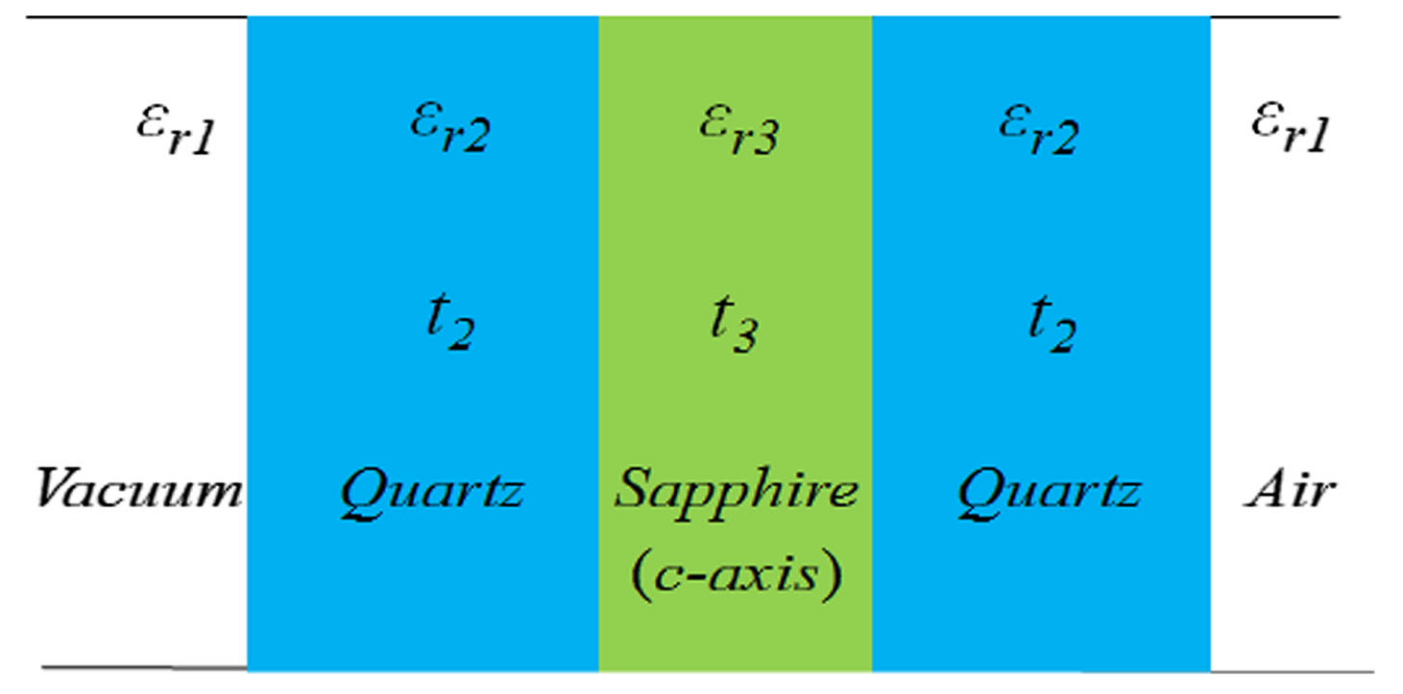
\includegraphics[width=0.25\textwidth]{pic/chapter1/多层介质.png} & 
        \hspace{5pt}
        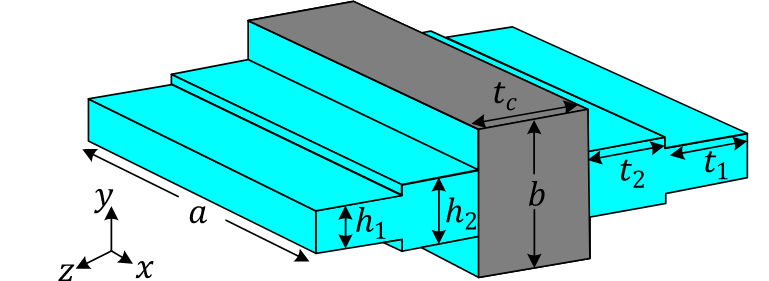
\includegraphics[width=0.45\textwidth]{pic/chapter1/窗片阶梯状形变.png}     \\
        \mbox{\small (a) 多层介质窗堆叠\citing{wang_broadband_window_2017}}                                                                               & 
        \mbox{\small (b) 窗片阶梯状形变\citing{liu_multilayer_broadband_2021}}                                                                                  \\[6bp]
        \multicolumn{2}{c}{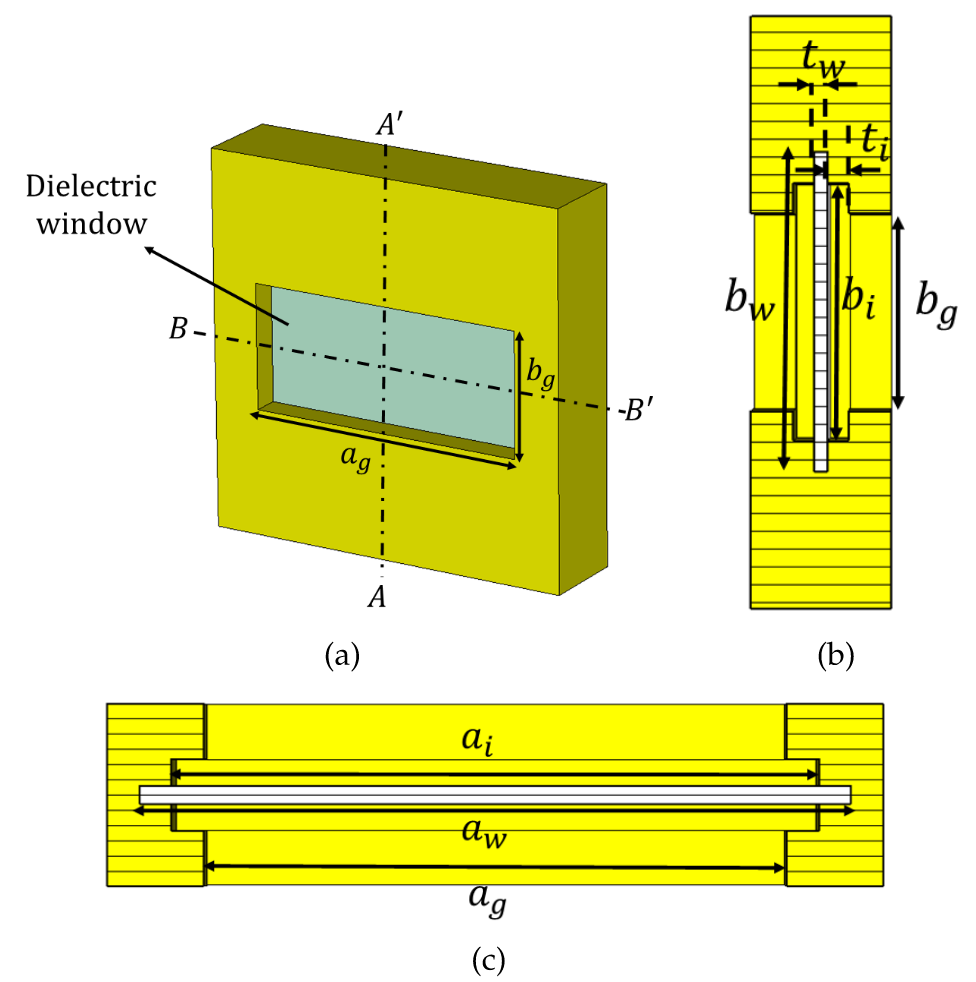
\includegraphics[width=0.3\textwidth]{pic/chapter1/匹配段阶梯过渡.png}} \\  % 使用跨列居中
        \multicolumn{2}{c}{\mbox{\small (c)匹配段阶梯过渡\citing{ali_multilayer_broadband_2020}}}
    \end{tabular}
    \caption{宽带多层匹配窗的常见设计方案}
    \label{fig:宽带多层匹配窗的常见设计方案}
\end{figure}

另外一种增加窗片带宽的方案是使用如图\ref{fig:布儒斯特窗}所示的布儒斯特窗\citing{sharan_broadening_2020,gantenbein_2014_brewster},将传统的单层圆窗片进行倾斜,达到介质的布儒斯特角并且获得极宽的带宽。原作者在这个方案中,使用了使用化学气相沉积法得到的钻石窗片,得到了在111.6-165.7GHz 范围内的回旋管中的十个不同模式均有不错的匹配效果的结果。布儒斯特窗相比于传统的盒型窗,不需要进行匹配段的设计,窗片的匹配与波导浑然一体。但是布儒斯特角的窗片为尺寸稍大于波导的倾斜焊接的椭圆形窗片,并且在装具焊接过程中部分窗片外露于波导之外。这使得布儒斯特窗在应力方面,相比于传统的圆形窗片更大。并且在加工焊接方面,由于要同时控制窗片的倾斜角与椭圆窗片长轴的朝向,对于装具焊接加工的精度要求更高。
\begin{figure}[!htb]
    \centering
    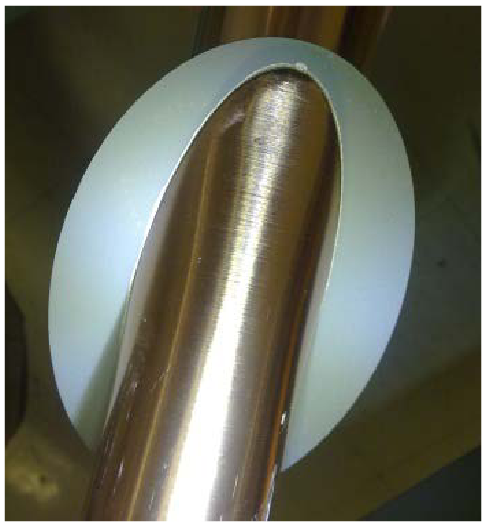
\includegraphics[width=0.3\textwidth]{pic/chapter1/布儒斯特窗.png}
    \caption{布儒斯特窗\citing{gantenbein_2014_brewster}}
    \label{fig:布儒斯特窗}
\end{figure}

随着设计工艺与制作加工工艺的发展,宽带宽真空器件产生的高功率与宽带宽微波辐射需求日益增长,这对微波窗的带宽提出了更高要求。经过前面宽带宽微波窗的设计方案调研,现阶段为了满足宽带宽匹配,微波窗的设计方案往往比较复杂。这不仅增加了制造成本,还影响了设备的紧凑性和后续加工的难度。在较高频段尤其是太赫兹范围,非常微小的装配与加工误差都会导致实际器件的性能的显著的下降。因此,此时需要一种结构较为简单紧凑,并且实现宽带宽匹配的微波窗结构。

\section{论文结构与安排}
本文主要设计了6-11GHz宽频带脊波导窗和L频段脊波导窗,并且进行了W频段圆波导窗的测试相关工作。

本文的主要结构安排如下:

第一章\hspace{6pt}绪论

本章首先概述了真空管的发展历程;紧接着,强调了微波窗在真空管中的重要性;之后,对常见微波窗的宽带方案进行了分析;并且基于上述分析,提出了设计紧凑小型化宽带微波窗的需求。

第二章\hspace{6pt}微波窗的理论研究

本章节首先分析了微波的等效电路分析法;并且对常见的微波传输线,尤其是脊波导传输线,进行了关于工作参数相关的分析;之后进行了传统盒型窗的理论研究;最后对常见的微波窗损毁机理进行了分析。

第三章\hspace{6pt}6-11GHz宽频带脊波导窗

本章节首先沿用上一章节的结论,分析了传统结构盒型窗的局限性;之后设计了一款6-11GHz宽频带脊波导窗;并且对此波导窗的参数敏感度进行了分析;然后分别使用最大场强法和二次电子发射法计算了波导窗的功率容量;之后对窗片进行了电热力多物理场仿真分析;最后为了方便后续的窗片测试对窗片进行了模式变换部分的设计。

第四章\hspace{6pt}L频段脊波导窗

本章节仿照上一章节将窗片搬移到L频段进行设计之后发现了窗片结构强度有所减弱的问题,之后对原先的结构在低频段的设计方面就进行了改进;然后分别使用最大场强法和二次电子发射法计算了波导窗的功率容量;最后对L频段的脊波导窗进行了多物理场分析。

第五章\hspace{6pt}W频段圆波导窗

在本章节中,首先以6-11GHz宽频带脊波导窗为例,探讨了安装过程中旋转误差对窗片性能参数的影响。接着,在实际测试W频段窗片时,发现了其与设计预期存在偏差的问题。针对这一问题,提出了若干假设,并利用HFSS软件进行了建模和仿真分析,仿真结果与假设揭示了W频段窗片焊接装具时候的问题所在。

第六章\hspace{6pt}总结与展望

在这部分中,我们首先回顾了整篇文章的主要内容,并对其存在的局限性进行了剖析,随后展望了未来的研究方向和工作安排。


\chapter{微波窗的理论研究}

\section{微波的等效电路分析}
为了寻求复杂的微波系统的传输特性,可以将其划分为均匀导波系统和非均匀微波元器件构成的复杂边界系统。通过使用传输线方程和结合实际的端接条件等数学手法,传输特定模式的电磁场的均匀导播系统可以被转化为传输线这一电路模型。由于相比于直接使用电磁场进行分析,电路相关的分析理论较为成熟,这一转化思想为分析复杂微波传输系统提供了良好的基础。
\subsection{常见微波传输线的特性阻抗}
在进行等效电路分析的时候,无论是进行阻抗匹配或者阻抗变换的设计还是进行特定的滤波器等无源器件的设计,,传输线的特性阻抗\(Z_C\)是一个非常重要的参数。现在先对常见的微波传输线的特性阻抗进行相应的分析。

同轴线是一种非常常见的传输线,其主要传输的模式是\(TEM\)模式,这种模式能够传输直流相关的信号,故其截止频率为0Hz。并且由于同轴线的次高模式的截止频率较高,此时同轴线的带宽也较宽。通过对同轴线上面的传输的基本模式\(TEM\)模式的电场与磁场进行相应的积分,可以求出其相应的特性阻抗\(Z_C\),其表达式为\ref{eq:同轴线的特性阻抗}。
\begin{equation}\label{eq:同轴线的特性阻抗}
    Z_C = \frac{60}{\sqrt{\varepsilon_r}} \ln \left( \frac{b}{a} \right)
\end{equation}
式子中,\(b, a\)分别为同轴线的外径和内径,\(\epsilon_r\)为同轴线填充均匀材料时的相对介电常数。但是在实际的应用过程中,为了兼顾同轴线系统的损耗与功率容量等因素的考虑,通常会将同轴线的特性阻抗\(Z_C\)取为\(50 \Omega\),这也是很多标准同轴线的特性阻抗。

矩形波导是一种常见的微波传输线,但是由于矩形波导的基本模式\(TE_{10}\)模式为\(TE\)模式,为了计算特性阻抗,对其传输模式的电场与磁场进行积分时候无法像\(TEM\)模式一样进行出现单值积分。故矩形波导以及后续传输非\(TEM\)模式的波导的特性阻抗结果都不唯一。具体的定义方法可以被分为电压-电流定义、功率-电压定义以及功率-电流定义。由于后续应用主要使用的是功率-电压定义,故本文如果不进行特别说明的话特性阻抗使用的便是波导传输在基本模式下以功率-电压定义的特性阻抗\(Z_{P, U}\)。此时根据文献\cite{heihil_characteristic_2006}中的计算,矩形波导的特性阻抗可以被表示为如式子\ref{eq:矩形波导的特性阻抗}中所示结果。

\begin{equation}\label{eq:矩形波导的特性阻抗}
    Z_{C}=  2\frac{b}{a} \cdot \frac{120 \pi \sqrt{\mu_r / \varepsilon_r}}{\sqrt{1 - \left( \frac{c}{2af \sqrt{\varepsilon_r \mu_r}} \right)^2}} 
\end{equation}
其中,\(b, a\)分别为矩形波导的长和宽,\(\mu_r, \varepsilon_r\)分别为矩形波导填充材料的相对磁导率和相对介电常数,\(c\)为真空中光的传播速度,\(f\)为矩形波导的工作频率,注意使用此公式时波导的工作频率应该高于截止频率。

圆柱形波导也是一种常见的微波传输线,并且其除了基本模式\(TE_{11}\)模式之外,其次高模式\(TE_{01}\)或者其它高次模式也因为一些特殊的极化特性而被广为使用,本次探讨的主要为其基本模式下的特性阻抗。此时,如果圆波导工作于\(TE_{11}\)模式下,其特性阻抗\(Z_C\)可以被表示为如式\ref{eq:圆柱波导的特性阻抗}所示结果。
\begin{equation}\label{eq:圆柱波导的特性阻抗}
    Z_{C}= 2.02 \cdot \frac{120 \pi \sqrt{\mu_r / \varepsilon_r}}{\sqrt{1 - \left( \frac{c}{3.413 \cdot Rf \sqrt{\varepsilon_r \mu_r}} \right)^2}} 
\end{equation}
此时R表示圆波导的半径,工作频率\(f\)依然应该高于截止频率。
\subsection{阻抗匹配设计}
阻抗匹配关系到微波系统的能量传输效率,并且针对不同的目的拥有不同的匹配方法。例如有的系统需要获得最低的输出噪声,此时需要针对性的进行最低噪声匹配。有的系统需要获得最高的传输效率,此时需要进行无反射匹配。有的系统需要输出端负载吸收最大功率,此时需要进行共轭匹配。良好的阻抗匹配能够减少系统的能量损失,其减少的能量损失转化的热量能增加整体系统的使用寿命。本文讨论的主要为无反射匹配,其主要匹配条件是波源与传输线之间的阻抗相同,即\(Z_s=Z_C\)。

在实际的微波系统中,经常因为各种各样的原因而产生不连续性,进而导致前后阻抗不匹配的情况。为了抑制这种不匹配,需要设计阻抗匹配方案,常见的有如下这几种解决方法:

1、单节阻抗变换器

如图\ref{fig:单节阻抗变换器}所示,此时输入特性阻抗为\(Z_C'\)的一节传输线被放置在了特性阻抗分别为\(Z_{C1}\)和\(Z_{C2}\)的两端传输线之间。为了实现前后两节传输线之间的阻抗匹配,此时可以将中间的传输线长度设置为传输线工作波长\(\lambda_g\)的四分之一,此时进行阻抗匹配的传输线的阻抗为\(Z_C'=\sqrt{Z_{C1} Z_{C2}}\)。
\begin{figure}[!htb]
    \centering
    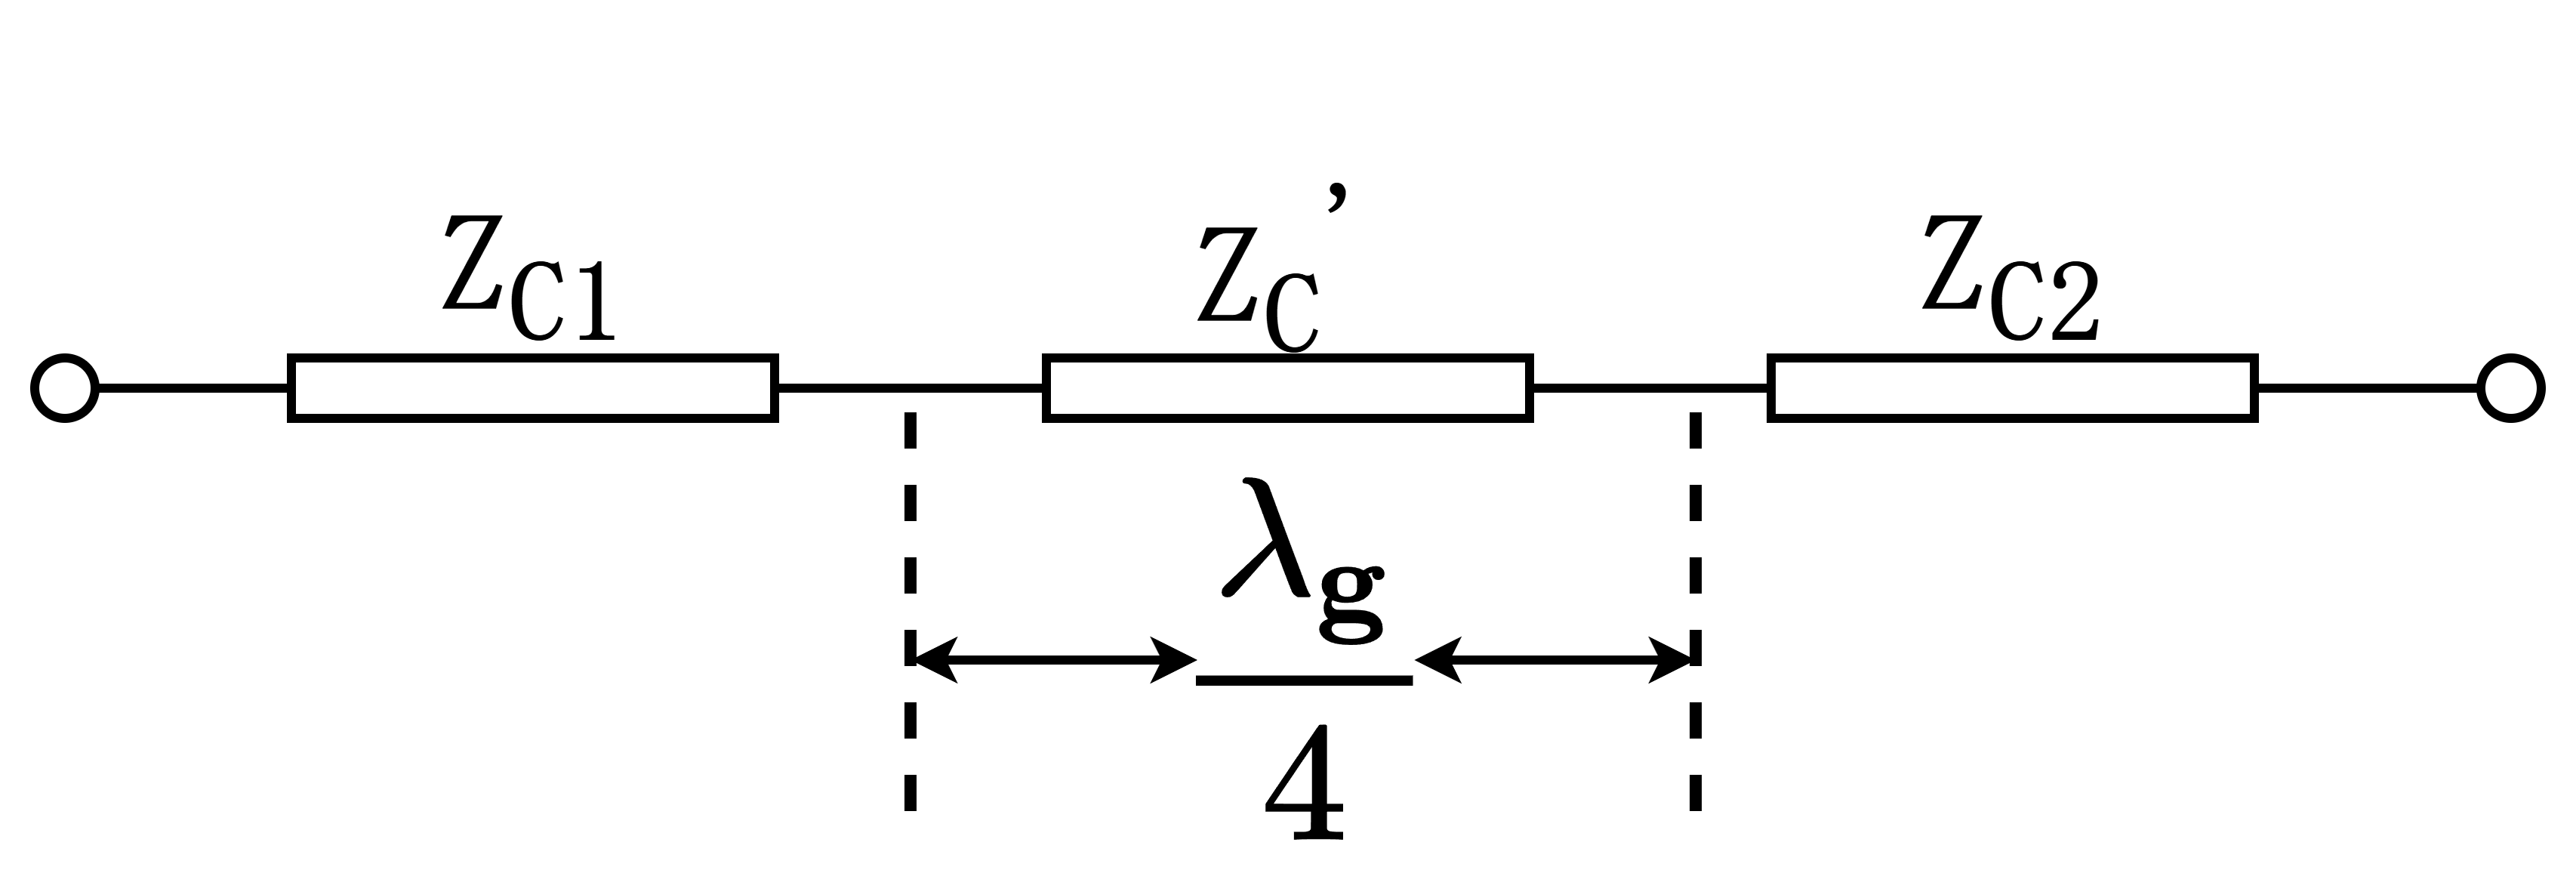
\includegraphics[width=0.5\textwidth]{pic/chapter2/单节阻抗变换器.png}
    \caption{单节阻抗变换器}
    \label{fig:单节阻抗变换器}
\end{figure}
单节阻抗变换器比较容易设计,但是其能够匹配的带宽太窄,不便于满足较宽带宽微波系统的需求,于是便衍生出来了另外的能够匹配较宽带宽的阻抗匹配方案。

2、多节阻抗变换器

为了实现带宽扩展,有必要扩充匹配段的节数,多节匹配段阻抗变换器的示意图如图\ref{fig:多节阻抗变换器}所示。现在假设此变换器由N段长度相同的传输线组成,第i段传输线的特性阻抗为\(Z_{C_i}\)。此时在第i段到第i+1段传输线处的反射系数\(\Gamma_i\)只考虑由于第i段到第i+1段之间的阻抗不匹配引起的反射,那么此时反射系数\(\Gamma_i\)满足的表达式如\ref{eq:多节阻抗变换器的反射系数}所示。
\begin{equation}\label{eq:多节阻抗变换器的反射系数}
    \Gamma_i = \frac{Z_{C_{i+1}}-Z_{C_{i}}}{Z_{C_{i+1}}+Z_{C_{i}}}
\end{equation}
关于端接处的两个反射系数\(\Gamma_0\)与\(\Gamma_L\)可以分别被表示为以下等式\ref{eq:端接处的反射系数}。
\begin{subequations}\label{eq:端接处的反射系数}
    \begin{align}
        \Gamma_0 &= \frac{Z_{C_1}-Z_{C_0}}{Z_{C_1}+Z_{C_0}} \\
        \Gamma_L &= \frac{Z_L-Z_{C_N}}{Z_L+Z_{C_N}}
    \end{align}
\end{subequations}
综合之前的结论,可以得知此时的总反射系数\(\Gamma\)可以被表示为式子\ref{eq:总反射系数表达式}所示。
\begin{equation}\label{eq:总反射系数表达式}
    \Gamma = \Gamma_0+\Gamma_1 \mathrm{e}^{2 j \theta}+\Gamma_2 \mathrm{e}^{4 j \theta}+...+\Gamma_N \mathrm{e}^{2 N j \theta}
\end{equation}
其中\(\theta = \beta l\)为每一小节的电长度,如果假设现在阻抗变换器是对称的,此时\(\Gamma_0 = \Gamma_N, \Gamma_1 = \Gamma_{N-1}, \dots \)
那么原式子\ref{eq:总反射系数表达式}可以被表达为\ref{eq:合并后的总反射系数表达式}所示的合并后的总反射系数表达式。
\begin{equation}\label{eq:合并后的总反射系数表达式}
    \Gamma = \mathrm{e}^{j  N \theta} \left[\Gamma_0\left(\mathrm{e}^{j N \theta}+\mathrm{e}^{- j N \theta} \right) + \Gamma_1\left(\mathrm{e}^{j (N-2) \theta}+\mathrm{e}^{- j (N-2) \theta} \right) + \dots \right]
\end{equation}
此时如果N为偶数,那么式子\ref{eq:合并后的总反射系数表达式}就有\(N/2\)项,如果N为记述,式子\ref{eq:合并后的总反射系数表达式}就有\((N-1)/2\)项。总而言之,此时\(\Gamma\)是一个关于\(\theta\)的傅里叶余弦级数式。通过增加总项数\(N\)以及调配每一段的\(Z_{C_i}\),可以将总反射系数\(\Gamma\)的幅值设计近似为任意所需要的函数,进而达到匹配的需求。
\begin{figure}[!htb]
    \centering
    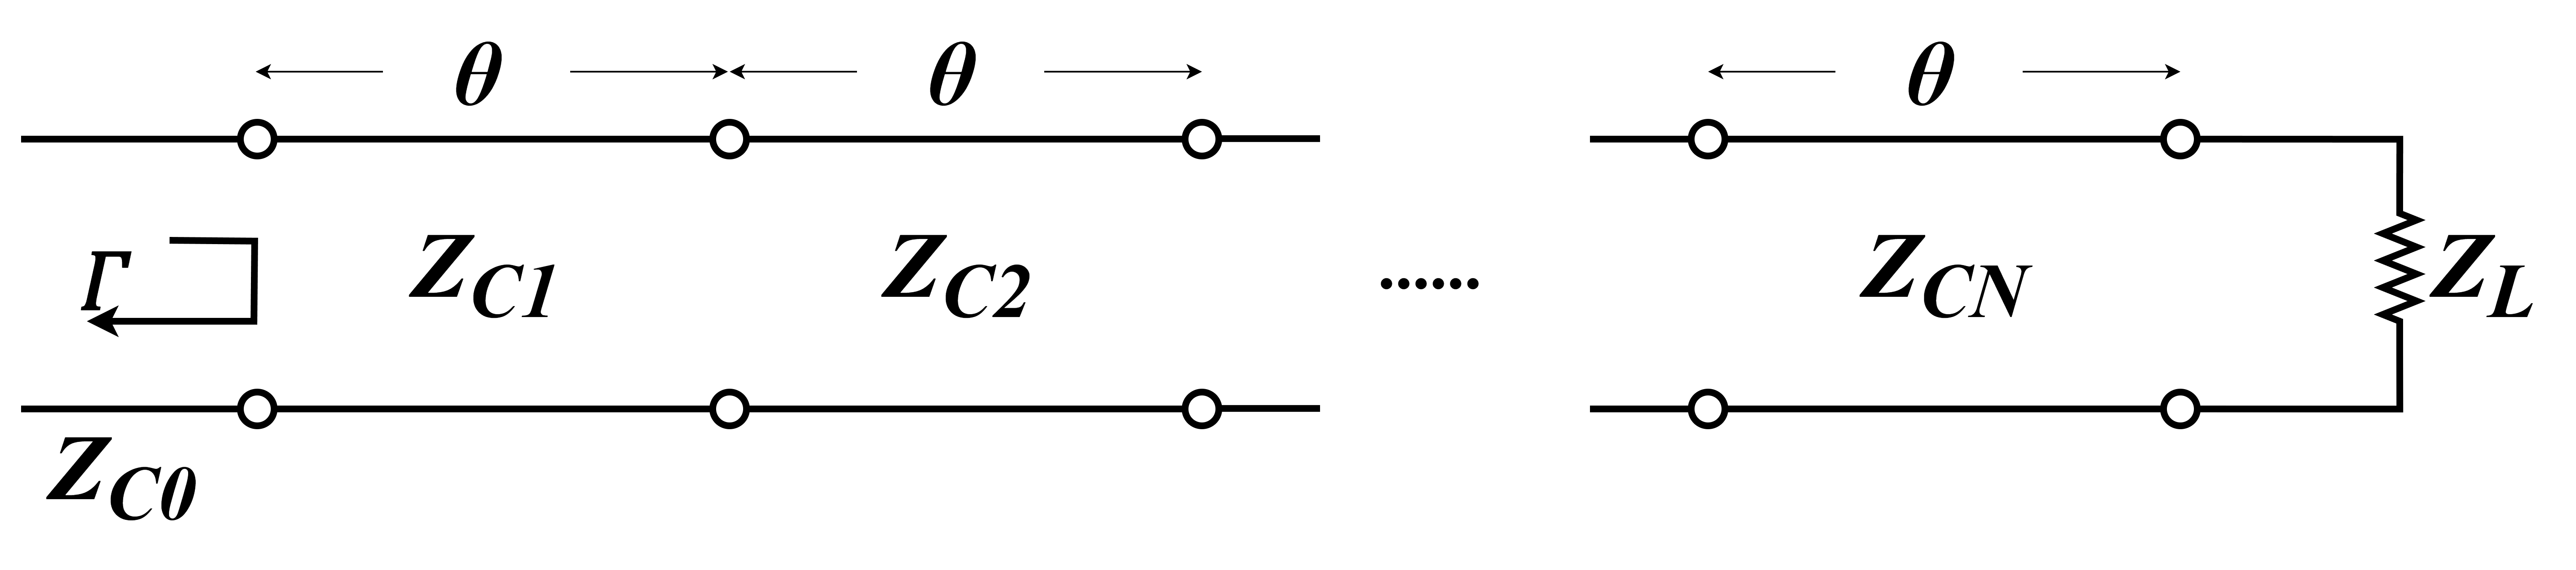
\includegraphics[width=0.75\textwidth]{pic/chapter2/多节阻抗匹配示意图.png}
    \caption{多节阻抗变换器}
    \label{fig:多节阻抗变换器}
\end{figure}


3、渐变阻抗变换器

如果将多节阻抗变换器的每一节的阻抗变换长度进一步的缩小,那么指定长度L的变换的节数会增加到无穷大,便可以构成渐变阻抗变换器,渐变阻抗变换器的示意图如图\ref{fig:渐变阻抗变换器}所示。假设阻抗变换的总长度为L,\(Z_S\)为输入端的传输线的特性阻抗,\(Z_L\)为输出端的传输线的特性阻抗,假设\(Z_S < Z_L \)。此时渐变段的特性阻抗沿着z的变化而变化,其为\(Z_C (z)\)。

那么此时应用小反射理论,可以得到\(z = 0\)处的总反射系数\(\Gamma_S\)的表达式如\ref{eq:渐变阻抗变换器的反射系数}所示\citing{davidmicrowave2015_continu}。
\begin{equation}\label{eq:渐变阻抗变换器的反射系数}
    \Gamma_S = \frac{1}{2} \int_{z=0}^{z=L} \mathrm{e}^{-2 j \beta z}\frac{d}{d z} \ln \left(\frac{Z_C}{Z_S}\right)  \,dz
\end{equation}
此时如果知道渐变段的\(Z_C(z)\)随着s\(z\)变化的值,那么便能实现带宽很宽的阻抗匹配。此时在实际的应用中,常见的渐变段的变化趋势有指数渐变、\(Klopfenstein\)渐变和三角形渐变等。
\begin{figure}[htbp]
    \centering
    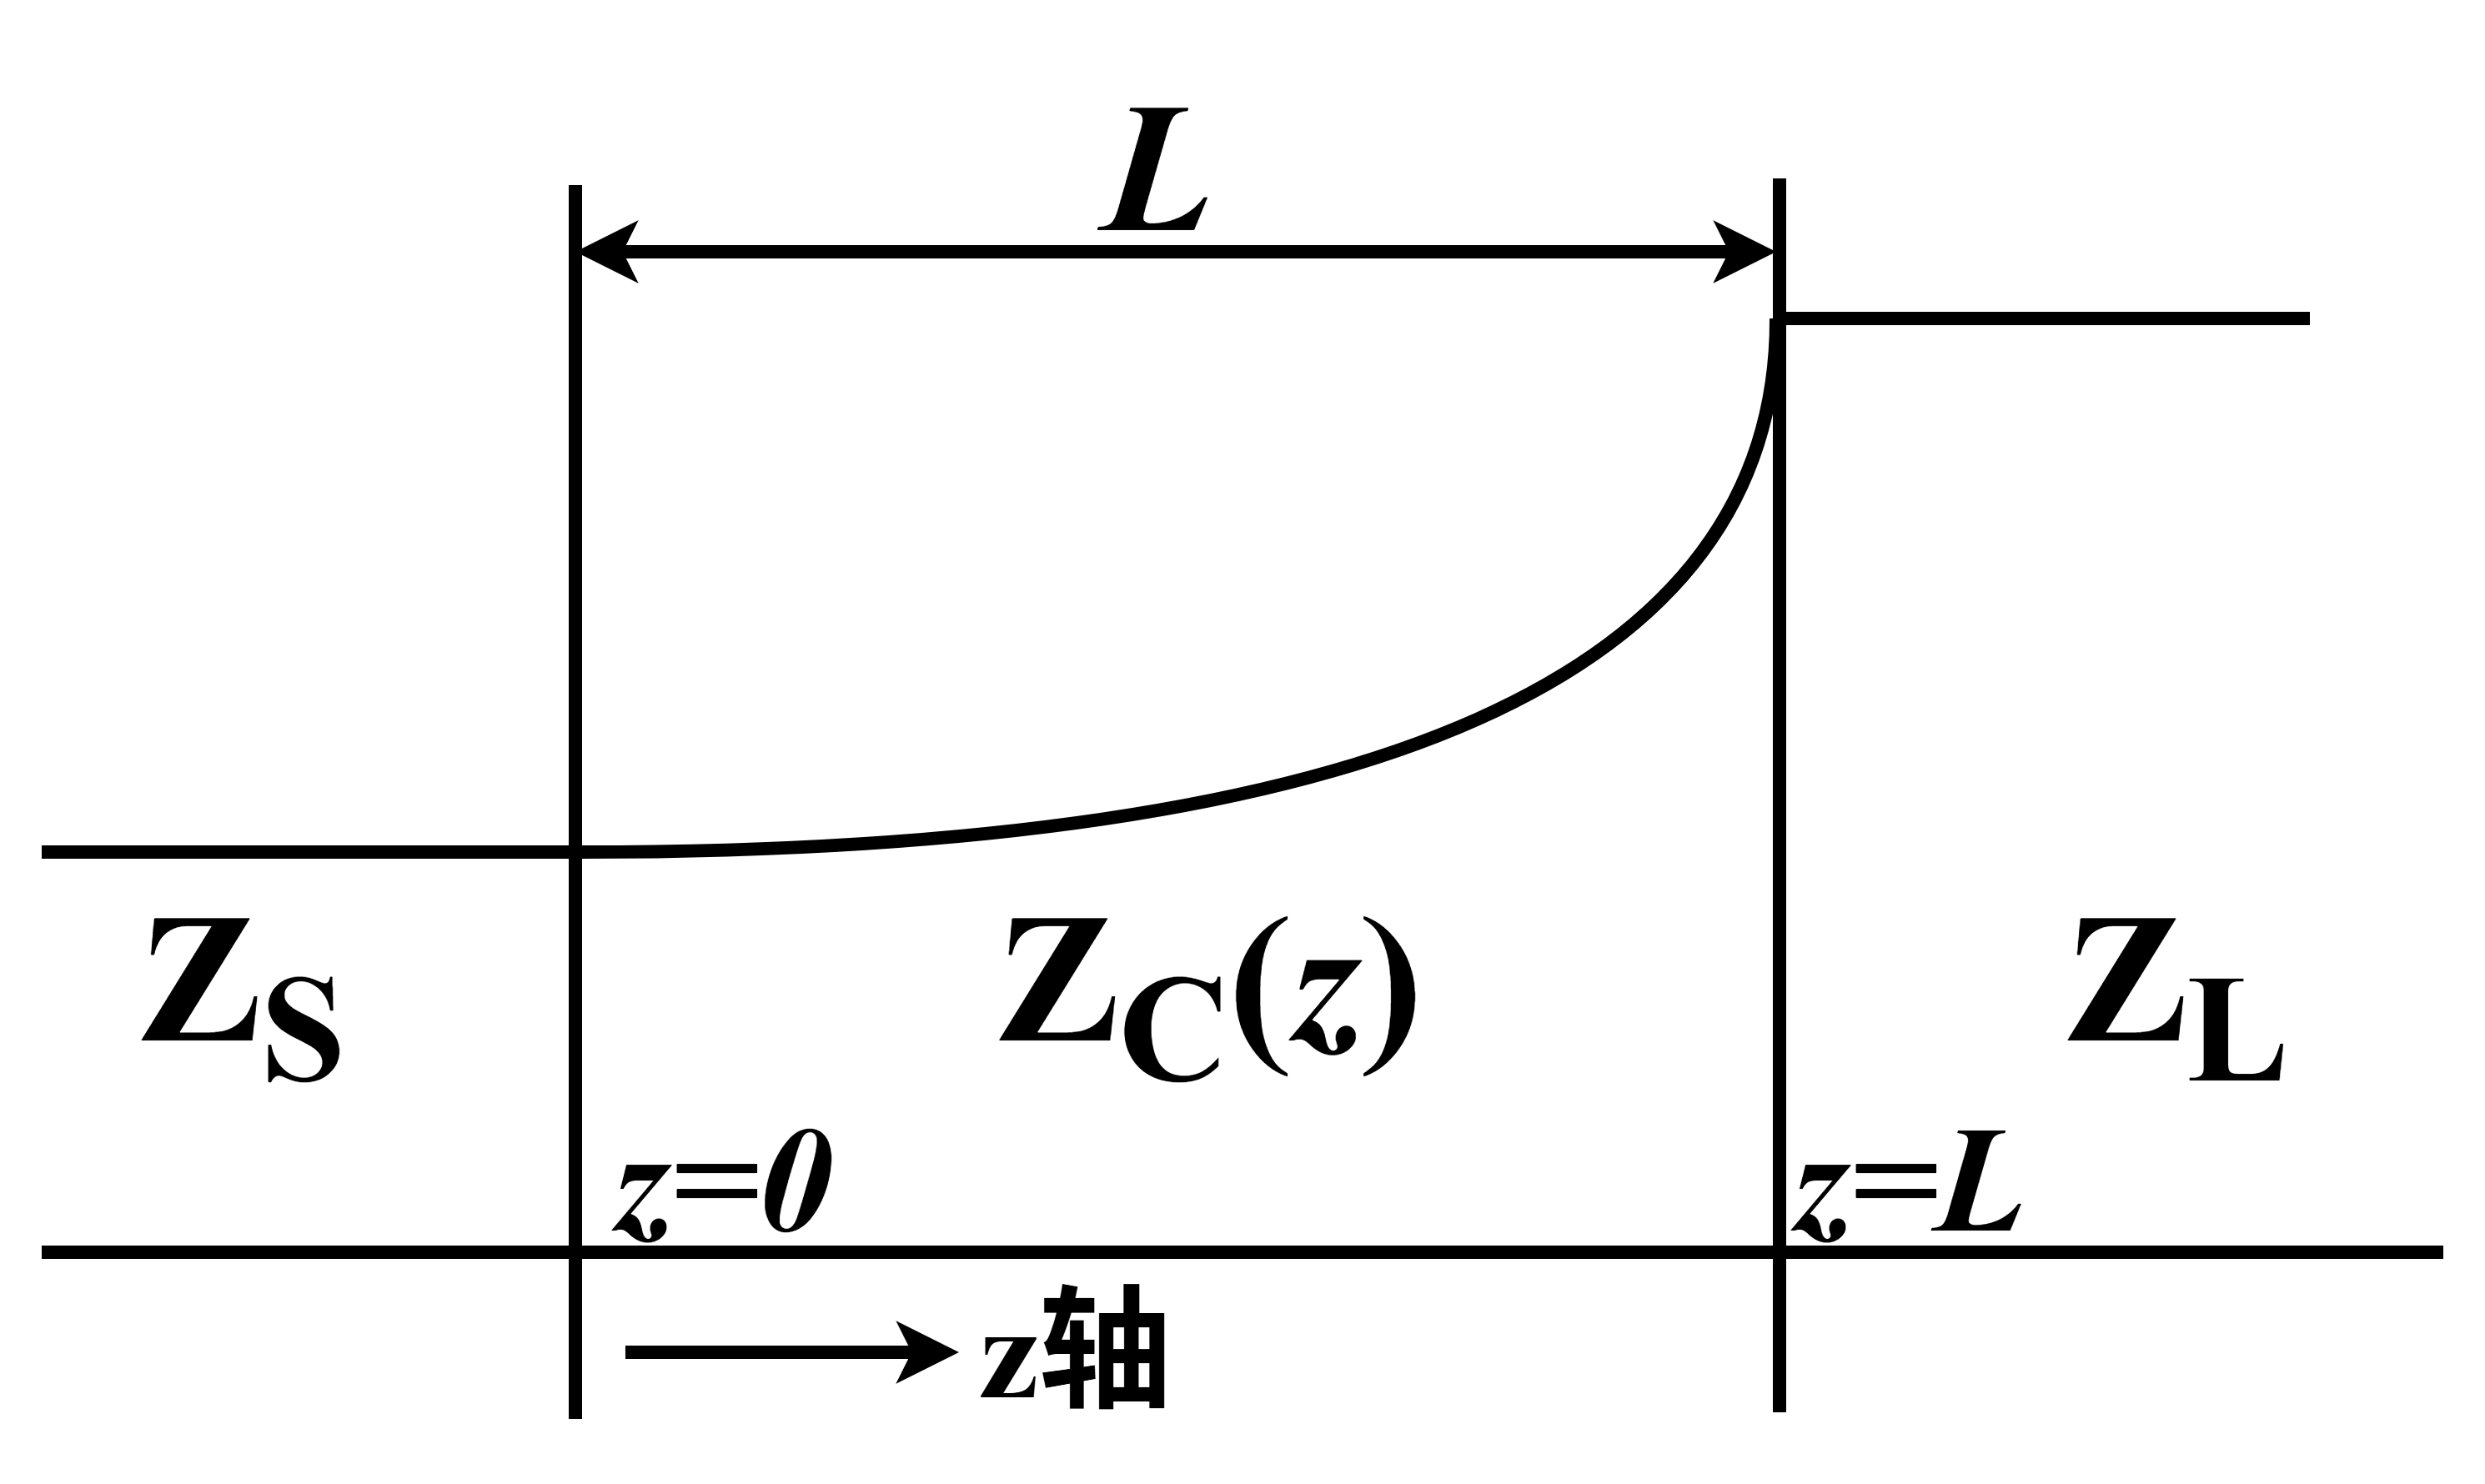
\includegraphics[width=0.5\textwidth]{pic/chapter2/渐变阻抗匹配示意图.png}
    \caption{渐变阻抗变换器}
    \label{fig:渐变阻抗变换器}
\end{figure}

\subsection{脊波导的工作特性与工作参数}\label{subsec:DoubleRidgeTheory}
脊波导由于其主模带宽非常宽,其经常由于优秀的几何结构特性便于被设计为过渡波导。并且由于其在真空填充时特性阻抗位于常用的标准矩形波导(377$\Omega$ )与同轴线(50$\Omega$)之间便于被设计为矩形波导与同轴线之间的过渡波导,故其是在许多宽带微波器件中常用的微波传输线之一\citing{helszajn_ridge_2000}。并且由于同频率之下的脊波导的长边长度要短于矩形波导,更加有利于器件的小型化。脊波导作为一种常见的宽带传输线,针对其主要的理论分析方法是横向谐振法(Transverse Resonance Method, TRM)。根据文献\cite{helszajn_double_ridge_2000, pingwang_double_ridge_2004,pingyingjiang_double_ridge_2007,hopefer_design_ridge_1955}使用横向谐振法可以分析出脊波导的截止频率、主模带宽以及其特性阻抗。需要注意的是,本文主要涉及以及本小节主要分析的脊波导为脊位于矩形波导长边或者短边正中间的对称情况,如果有不对称脊波导的需求的话,可以参考文献\cite{ramesh_asymmetri_2001}中的求解方法进行分析。

脊波导传输的基本模式是主模类$TE_{10}$模式,其次高模式为类$TE_{20}$模式,为了分析这两个模式的截止频率,有必要画出脊波导在横向上的等效电路。其中,脊两边的空隙可以分别被等效为两端传输线,脊凸起的平台也可以被等效为一段传输线,凸起的脊的两侧所引入的不连续性由于会与对侧的脊或者底边产生电势差,故可以分别被等效为两端电容。当模式截止时,根据横向谐振法,相当于横向的等效电路陷入谐振情况。此时以脊的左侧为参考平面,假设向左看得到的等效导纳为$Y_{1}$,向右看得到的等效导纳为$Y_{2}$,如果产生了横向谐振那么可以得到横向谐振方程\ref{eq:Y1Y2}:
\begin{equation}\label{eq:Y1Y2}
    Y_{1}=-Y_{2}
\end{equation}

以此为基础,我们可以得到分析脊波导的截止频率的横向谐振方程\ref{eq:TRM_DW}:
\begin{equation}\label{eq:TRM_DW}
    -\cot \theta_1 + \left( \frac{Y_{02}}{Y_{01}} \right) \tan \theta_2 + \frac{B}{Y_{01}} = 0 
\end{equation}
其中参数可被表示为等式\ref{eq:TRM_DW_parameters}中的\ref{eq:Y01}到\ref{eq:BY01}:
\begin{subequations}\label{eq:TRM_DW_parameters}
    \begin{align}
    Y_{01} &= \frac{k_c}{\omega \mu_0} \left( \frac{1}{b} \right) \label{eq:Y01} \\
    Y_{02} &= \frac{k_c}{\omega \mu_0} \left( \frac{1}{d} \right) \label{eq:Y02} \\
    \theta_1 &= \frac{\pi (a - s)}{\lambda_c} = \pi \left( 1 - \frac{s}{a} \right) \left( \frac{a}{\lambda_c} \right) \label{eq:theta1} \\
    \theta_2 &= \frac{\pi s}{\lambda_c} = \pi \left( \frac{s}{a} \right) \left( \frac{a}{\lambda_c} \right) \label{eq:theta2} \\
    \frac{B}{Y_{01}} & \approx 2 \delta_{r} \left( \frac{b}{a} \right) \left( \frac{a}{\lambda_c} \right) \ln \csc \left( \frac{\pi d}{2b} \right) \label{eq:BY01}
    \end{align}
\end{subequations}
式子\ref{eq:TRM_DW_parameters}中的参数定义如下:$a$为脊波导长边长,$b$为脊波导短边长,$s$为脊的宽度,$d$为脊凸起后留下的空腔缝隙宽度。$\delta_{r}$为与脊波导相关的几何系数:双脊波导时$\delta_{r}=1$,单脊波导时$\delta_{r}=2$。$\omega$为当前角频率;$\mu_0$为真空磁导率。波导截止波数$k_c=2\pi / \lambda_c$,截止波长$\lambda_c$在真空填充脊波导时与截止频率$f_c$满足$\lambda_c=c/f_c$。$Y_{01}$为脊两侧空腔所引入的导纳,$Y_{02}$为脊所引入的导纳,$\frac{B}{Y_{01}}$为脊引入电纳按照$Y_{01}$进行归一化之后的结果。

此时如果式子\ref{eq:BY01}中的对数函数套三角函数造成超越方程以至于难以求解,可以使用近似替代公式\ref{eq:ln_csc}:
\begin{equation}
    \ln \csc \left( \frac{\pi \alpha}{2} \right) \approx \frac{1}{2} \left[ \left( \frac{1 + \alpha^2}{\alpha} \right) \ln \left( \frac{1 + \alpha}{1 - \alpha} \right) - 2 \ln \left( \frac{4 \alpha}{1 - \alpha^2} \right) \right] \label{eq:ln_csc}
\end{equation}
其中,$\alpha=d/b$,为脊的空隙与脊波导短边之比。

关于双脊波导的截止频率有近似的显式解\citing{Hoefer1982AnalyticalEF},如果双脊波导的几何形状满足以下约束关系\ref{eq:DRW_constraints}:
\begin{equation}\label{eq:DRW_constraints}
    \begin{aligned}
    0.01 &\leq \frac{d}{b} \leq 1 \\
    0 &\leq \frac{b}{a} \leq 1 \\
    0 &\leq \frac{s}{a} \leq 0.45
    \end{aligned}
\end{equation}
使用式子\ref{eq:DRW_closed}求解时候的误差小于1\%

\begin{equation}\label{eq:DRW_closed}
    \begin{split}
        \frac{a}{\lambda_c} = \frac{a}{2(a - s)} & \left[ 1 + \frac{4}{\pi} \left( 1 + 0.2 \sqrt{\frac{b}{a - s}} \right) \left( \frac{b}{a - s} \right) \ln \csc \left( \frac{\pi d}{2b} \right) \right. \\
        & \left. + \left( 2.45 + 0.2 \frac{s}{a} \right) \left( \frac{sb}{d(a - s)} \right) \right]^{-\frac{1}{2}}
    \end{split}
\end{equation}

配合MATLAB或者Mathematica等数学软件,可以对以上式子进行数值求解,进而得到给定几何参数下的脊波导的截止频率。这些公式对要设计一个指定截止频率的脊波导的情况,也有着不错的先验能力。

脊波导跟其他波导类似,其特性阻抗有着不同的定义方式,这里主要介绍电压-电流定义的特性阻抗与功率-电压定义的特性阻抗。根据文章\cite{Hoefer1982AnalyticalEF}的描述,脊波导的电压-电流定义的特性阻抗\(Z_C\)可以被描述为等式\ref{eq:脊波导电压-电流定义的特性阻抗}中的定义。
\begin{equation}\label{eq:脊波导电压-电流定义的特性阻抗}
    Z_C = Z_{\mathrm{VI}}(\infty) \cdot \frac{1}{\sqrt{1-(f/f_c)^2}}
\end{equation}
其中式子\ref{eq:脊波导电压-电流定义的特性阻抗}中的因子\(Z_{\mathrm{VI}}(\infty)\)可以根据式子\ref{eq:Z_IV}进行计算:
\begin{equation}\label{eq:Z_IV}
    Z_{\mathrm{VI}}(\infty) = \left( \frac{b}{a} \right) \left( \frac{d}{b} \right) \left( \frac{a}{\lambda_c} \right) \frac{\pi \eta_0}{\sin \theta_2 + \left( \frac{d}{b} \right) \left[ \frac{B}{Y_{01}} + \tan \left( \frac{\theta_1}{2} \right) \right] \cos \theta_2}
\end{equation}
式子中的参数已经在\ref{eq:TRM_DW_parameters}中被定义过,其中$\eta_0$为真空波阻抗。本公式单脊波导或者双脊波导都可以套用,区别为截止频率不同以及\ref{eq:BY01}中定义的$\delta_{r}$不同。

脊波导的功率-电压定义的特性阻抗\(Z_C\)与因子的\(Z_{\mathrm{PV}}(\infty)\)的关系跟等式\ref{eq:脊波导电压-电流定义的特性阻抗}中的关系类似,此时因子\(Z_{\mathrm{PV}}(\infty)\)可以根据式子\ref{eq:Z_PV}进行计算:
\begin{equation}\label{eq:Z_PV}
    Z_{\mathrm{PV}}(\infty) = \frac{\pi \eta_0 \left( \frac{b}{a} \right) \left( \frac{d}{b} \right) \left( \frac{a}{\lambda_c} \right)}{
        \left\{ 
            \begin{aligned}
                & \left( \frac{d}{b} \right) \left( \frac{b}{a} \right) \left( \frac{2 \delta_r a}{\lambda_c} \right) \ln \csc \left( \frac{\pi d}{2b} \right) \cos^2 \theta_2 + \frac{\theta_2}{2} + \frac{\sin 2\theta_2}{4} \\
                & + \left( \frac{d}{b} \right) \left( \frac{\cos \theta_2}{\sin \theta_1} \right)^2 \left[ \frac{\theta_1}{2} - \frac{\sin 2\theta_1}{4} \right]
            \end{aligned}
        \right\}
    }
\end{equation}
式子中的$\delta_{r}$与之前\ref{eq:BY01}中的定义相同,在单脊波导中取2,在双脊波导中取1。其余参数也与\ref{eq:TRM_DW_parameters}中的定义相同。

\section{盒型窗的理论研究与验证}\label{sec:PillBoxTheory}
随着时代的发展,微波窗的种类也趋于多种多样,在理论研究方面比较完备的微波窗是盒型窗与同轴窗,这两种窗的结构较为简单便于使用场匹配或者等效电路法进行研究。由于对这两种窗的结构理论研究有助于后续的窗片设计,故现在此对这两种窗的基本理论进行相应的论述。
常见的盒型窗的主要是由负责进行传输的矩形波导、一个薄圆片形状的介质窗片以及窗片两侧的匹配圆柱波导组成,这其中蕴含了的电磁场边界条件的不连续性,可以使用等效电路法来进行研究。此时将盒型窗的两侧波导以及窗片两侧的空气圆柱部分等效为波导传输线,将较为薄的窗片、矩形波导与圆柱形波导之间的不连续性和窗片与圆柱形波导之间的不连续性等效为电纳。并以此等效思路为基础构建微波窗的等效电路,进而求解电路的频率响应。

常规的盒型窗的矩形波导的工作频率为$TE_{10}$模式,其中的圆形窗片的主要工作模式为$TE_{11}$模式,这两种模式均为波导的基模。当矩形波导和圆波导进行直接耦合的时候根据文章\citing{Bharathi2015DESIGNAD, marcuvitz_waveguide_1986_rec_cylinder}的研究表明,此时会出现不连续性,在等效电路中相当于引入了一个等效电纳$B_{T}$,此时根据式子\ref{eq:B_T}这个等效电纳可以被表示为:
\begin{equation}\label{eq:B_T}
    B_{T}=\frac{b}{\lambda_{g r}}\left\{2 \ln \left(\frac{D^{2}-b^{2}}{4 b D}\right)+\left(\frac{b}{D}+\frac{D}{b}\right) \ln \left(\frac{D+b}{D-b}\right)+2 \sum_{n=1}^{\infty} \frac{\sin ^{2} n \phi}{n^{3} \phi^{2}} \delta_{2 n}\right\}
\end{equation}
此时式子中的$D$为圆形波导的直径,$a$和$b$分别为矩形波导的长边长度和短边长度,$\beta$为矩形波导的传播常数,$\lambda_{g r}$为矩形波导的工作波长,$\lambda_{g c}$为圆形波导的工作波长,$t$为圆柱形介质窗片的厚度,$\omega$为微波窗的角工作频率,$c$为真空的光速,$\lambda$为自由空间中的波长。

为了便于封装焊接,窗片的直径最好等于矩形波导的对角线长度,此时根据勾股定理我们可以得到窗片直径$D$和矩形波导长短边之间的关系$D=\sqrt{a^2+b^2} $。关于计算式最后的求和式中的$\delta_{2n}$和$\phi$的计算方法可以被表示为式子\ref{eq:delta_phi}中的\ref{eq:delta}到\ref{eq:phi}所示:
\begin{subequations}\label{eq:delta_phi}
\begin{align}
    \delta_{2 n} &= \frac{1}{\sqrt{1-\left(\frac{\beta \mathrm{D}}{2 \pi n}\right)^{2}}}-1 \label{eq:delta}\\
    \beta &= \frac{2 \pi}{\lambda_{gr}} \label{eq:beta}\\
    \phi &= \frac{\pi b}{D} \label{eq:phi}
\end{align}
\end{subequations}
根据之前分析的盒型窗中存在的三个不连续性边界条件,可以将原先的盒型窗等效为如--所示的等效电路,在这个等效电路中,$Z_{cir}$是真空填充的圆柱形波导的特征阻抗,$Z_{rec}$是矩形波导的特征阻抗,$B_{d}$是圆形窗片引入不连续性所等效的归一化电纳,$B_{T}$是由于矩形波导与圆柱形波导之间的不连续性引入的归一化电纳。

根据微波网络理论,这个两端口的等效电路可以被表示为一个如\ref{eq:ABCD}所示的$ABCD$矩阵,其中$k=Z_{cir}/Z_{rec}$,是真空填充的圆柱形的特征阻抗按照矩形波导的特征阻抗所归一化的特征阻抗比值;$\gamma=\frac{2 \pi}{\lambda_{gc}}$是真空填充的圆柱形波导的传播常数,$l$是介质窗片两侧的真空填充的圆柱形波导的纵向长度。
\begin{equation}\label{eq:ABCD}
    \begin{split}
        \begin{bmatrix}
            A & B \\
            C & D
        \end{bmatrix} 
        & = 
        \begin{bmatrix}
            \sqrt{k} & 0 \\
            jB_{T}\sqrt{k} & 1/\sqrt{k}
        \end{bmatrix}
        \begin{bmatrix}
            \cos{\gamma l} & j\sin{\gamma l} \\
            j\sin{\gamma l} & \cos{\gamma l}
        \end{bmatrix}
        \begin{bmatrix}
            1 & 0 \\
            jB_{d} & 1
        \end{bmatrix} \\
        & \quad \times 
        \begin{bmatrix}
            \cos{\gamma l} & j\sin{\gamma l} \\
            j\sin{\gamma l} & \cos{\gamma l}
        \end{bmatrix}
        \begin{bmatrix}
            1/\sqrt{k} & 0 \\
            jB_{T}\sqrt{k} & \sqrt{k}
        \end{bmatrix}
    \end{split}
\end{equation}

由于此时的窗片的厚度相比于使用窗片介质填充的圆柱形波导的工作波长来说太短,其引入的不连续性可以被等效为电纳$B_{d}$,详细的计算式是式\ref{eq:B_d},其中$t$为窗片的厚度,$\varepsilon_d$为窗片的相对介电常数:
\begin{equation}\label{eq:B_d}
    B_{d} = t (\varepsilon_d - 1) \left( \frac{\omega}{c} \right) \left( \frac{\lambda_{gc}}{\lambda} \right)
\end{equation}

此时,假设盒型窗的输入功率为$P_{1}$,通过盒型窗之后输出功率为$P_{2}$,根据S参数以及$ABCD$矩阵的定义,我们可以得到$P_{2}$与$P_{1}$的比值为式子\ref{eq:P2P1}:
\begin{equation}\label{eq:P2P1}
    \frac{P_{2}}{P_{1}} = \frac{1}{1+\frac{1}{4} (B-C)^2}
\end{equation}
那么根据能量守恒定律,假设窗片不存在损耗,那么其反射系数$|\Gamma|$可以被表示为式子\ref{eq:Gamma}:
\begin{equation}\label{eq:Gamma}
    |\Gamma| = \left| 1 - \left( \frac{P_{2}}{P_{1}} \right) \right|^{\frac{1}{2}}
\end{equation}
假设窗片完全传输,那么此时的$P_{2}=P_{1}$,进而根据式子\ref{eq:P2P1}可以推理出来$ABCD$矩阵中的$B=C$。为了获得一个可以确定盒型窗的几何参数的进行求解的方程,有必要进行几点假设:
\begin{enumerate}
    \item 此时的真空填充的圆柱形波导的长度$l$可以较为任意的进行选取,注意是较为任意的选取不是完全任意的选取,因为如果真空填充的圆柱形波导的长度过短,会导致圆柱形波导部分无法被等效为一段传输线,进而导致原先的等效电路模型失效。
    \item 窗片的材料已经确定,也就是窗片的相对介电常数$\varepsilon_{d}$是一定的。
    \item 要求匹配到的频点$f$为已经确定的值,也就是$\lambda$、$\lambda_{gc}$和$\lambda_{gr}$是已经确定的。
\end{enumerate}


现在我们将原先式子\ref{eq:ABCD}的几个矩阵元素完全相乘,可以得到计算式\ref{eq:ABCD_solved},式子中\ref{eq:A}到\ref{eq:D}为计算式\ref{eq:ABCD}中$ABCD$矩阵的四个元素:
\begin{subequations}\label{eq:ABCD_solved}
    \begin{align}
        A &= \frac{1}{2} \big[-(B_d + 2 B_T k) \sin(2\gamma l) + (2 - B_d B_T k)\cos(2\gamma l) + B_d B_T k \big] \label{eq:A} \\
        B &= -i k \sin(\gamma l) (B_d \sin(\gamma l) - 2 \cos(\gamma l)) \label{eq:B} \\
        C &= \frac{i (\cos(\gamma l) - B_T k \sin(\gamma l)) \big[(2 - B_d B_T k)\sin(\gamma l) + (B_d + 2 B_T k)\cos(\gamma l)\big]}{k} \label{eq:C} \\
        D &= \frac{1}{2} \big[-(B_d + 2 B_T k) \sin(2\gamma l) + (2 - B_d B_T k)\cos(2\gamma l) + B_d B_T k \big] \label{eq:D}
    \end{align}
\end{subequations}

注意到推演结果中$A$元素与$D$元素相等,这与微波网络中的理论描述相符。此时为了满足$ABCD$矩阵的$B$与$C$元素相等,我们可以将这两个元素进行作差处理,如果相等的话那么可以得到$B-C=0$,进一步的,可以得到如下关于作差后的表达式\ref{eq:B-C-simplify1}:

\begin{equation}\label{eq:B-C-simplify1}
    \begin{split}
        B - C = & -\frac{i}{2k} \Bigg( \Big[-B_{d}(B_{T}^2 + 1)k^2 + B_{d} + 4B_{T}k\Big]\cos(2\gamma l) 
                  + B_{d}(B_{T}^2 + 1)k^2 \\
                & - 2\Big\{k\big[B_{T}(B_{d} + B_{T}k) + k\big] - 1\Big\}\sin(2\gamma l) 
                  + B_{d} \Bigg) \\
                = & -\frac{i}{2k} \Bigg(B_{d}(B_{T}^2 + 1)k^2(1-\cos(2\gamma l)) + B_{d}(1+\cos(2\gamma l)) \\
                & +4B_{T}k\cos(2\gamma l) - 2\Big\{k\big[B_{T}(B_{d} + B_{T}k) + k\big] - 1\Big\}\sin(2\gamma l) \Bigg) = 0
    \end{split}
\end{equation}

此时在表达式\ref{eq:B-C-simplify1}中,在两边约去$-\frac{i}{2k} $后,在两边同时乘以$\frac{\tan(\gamma l)}{\sin(2 \gamma l)}$,运用倍角公式并且进行整理后可以得到式子\ref{eq:B-C-simplify1}的等价形式\ref{eq:B-C-simplify2},也就是:
\begin{equation}\label{eq:B-C-simplify2}
    \begin{split}
     & k \big[B_{d}(B_{T}^2+1)k - 2B_{T}\big]\tan^2(\gamma l) 
       + \Big\{ 2- 2k\Big[B_{T}\big(B_{d} + B_{T}k\big) + k\Big] \Big\}\tan(\gamma l) \\
    & + B_{d} + 2B_{T}k = 0
    \end{split}
\end{equation}

假设真空填充的圆柱形波导的长度$l$是可以任意选取的,并且此时的要求频点已经确定,式子\ref{eq:B-C-simplify2}确定了一个关于$\tan(\gamma l)$的一元二次方程,要求情况下的盒型窗有存在的参数的充分必要条件是这个一元二次方程有解,那么此时可以确定的是这个方程的$\Delta >0$,这个非常的$\Delta$可以得到式子\ref{eq:Delta}:
\begin{equation}\label{eq:Delta}
    \Delta = 4 - 4 (2 + B_{d}^2 - 2 B_{T}^2) k^2 + 4 (1 + B_{T}^2)^2 k^4>0
\end{equation}

此时$\Delta$中,$B_{T}$为矩形波导与圆波导直接耦合的归一化电纳,$k$为真空填充的圆柱形波导的特征阻抗按照矩形波导的特征阻抗所归一化的特征阻抗比值。这两条均为随着矩形波导的尺寸选取进而已经确定的数值。$B_{d}$为窗片引入的归一化电纳,其与窗片的厚度$t$相关。

那么盒型窗的标准设计流程便已经确定了:
\begin{enumerate}
    \item 确定匹配的频点$f$。
    \item 根据频点选取合适的矩形波导尺寸以及窗片的材料进而得到盒型窗的几何尺寸$a, b, D$与窗片的相对介电常数$\varepsilon_{d}$。
    \item 使用微波工程的相关知识,分别计算矩形波导与圆柱形波导在匹配频点的工作波长($\lambda_{gr}, \lambda_{gc}$)与特性阻抗($Z_{rec}, Z_{cir}$),为接下来的计算做好准备。
    \item 使用式子\ref{eq:B_T}计算矩形波导与圆柱形波导之间不连续性引入的电纳$B_T$,在实际的应用过程中后方无线求和式子项数可以取为5。使用式子\ref{eq:B_d}和不等式\ref{eq:Delta}判断窗片厚度$t$的取值范围。
    \item 综合考量解的存在性、加工的难易程度以及机械结构的牢固性之后选取一个合适的窗片厚度$t$,之后使用软件找到超越方程\ref{eq:B-C-simplify2}关于真空填充的圆柱形波导$l$的长度的解
    \item 此时考量圆柱形波导$l$的长度,并且计算电长度$l / \lambda_{gc}$,在实际的仿真计算的验证过程中可以验证到此时其电长度最好不要低于0.1,不然的话会因为圆柱形波导无法被等效为传输线进而导致原先的等效电路模型失效而产生匹配频点出现频偏。
    \item 使用电磁仿真软件进行建模,验算刚才的参数,并且使用优化进而得到最佳的参数。
\end{enumerate}

现在以工作频段为6.57 -9.99 GHz 的标准矩形波导WR112为例子,使用本章节中的盒型窗理论编写Python代码,匹配中心频点8.28 GHz 的传统盒型窗。此时选择窗片的材料为相对介电常数为\( \varepsilon_r = 9.4\)的蓝宝石进行匹配。在进行运算之后,得到窗片的厚度wt与匹配段纵向长度trh之间的对应关系如图\ref{fig:传统盒型窗匹配长度与窗片厚度关系}所示。此时图中的橙黄色区域蓝宝石窗片厚度低于0.6mm,会使得蓝宝石窗片的焊接后的气密性降低,并且会影响窗片机械强度。图中灰色区域床波段电长度小于0.1,会使得按照计算参数进行设计的盒型窗的匹配频点出现频偏。故此时应该在没有被橙色区域与灰色区域覆盖的区域选择蓝色点进行设计。
\begin{figure}[!htb]
    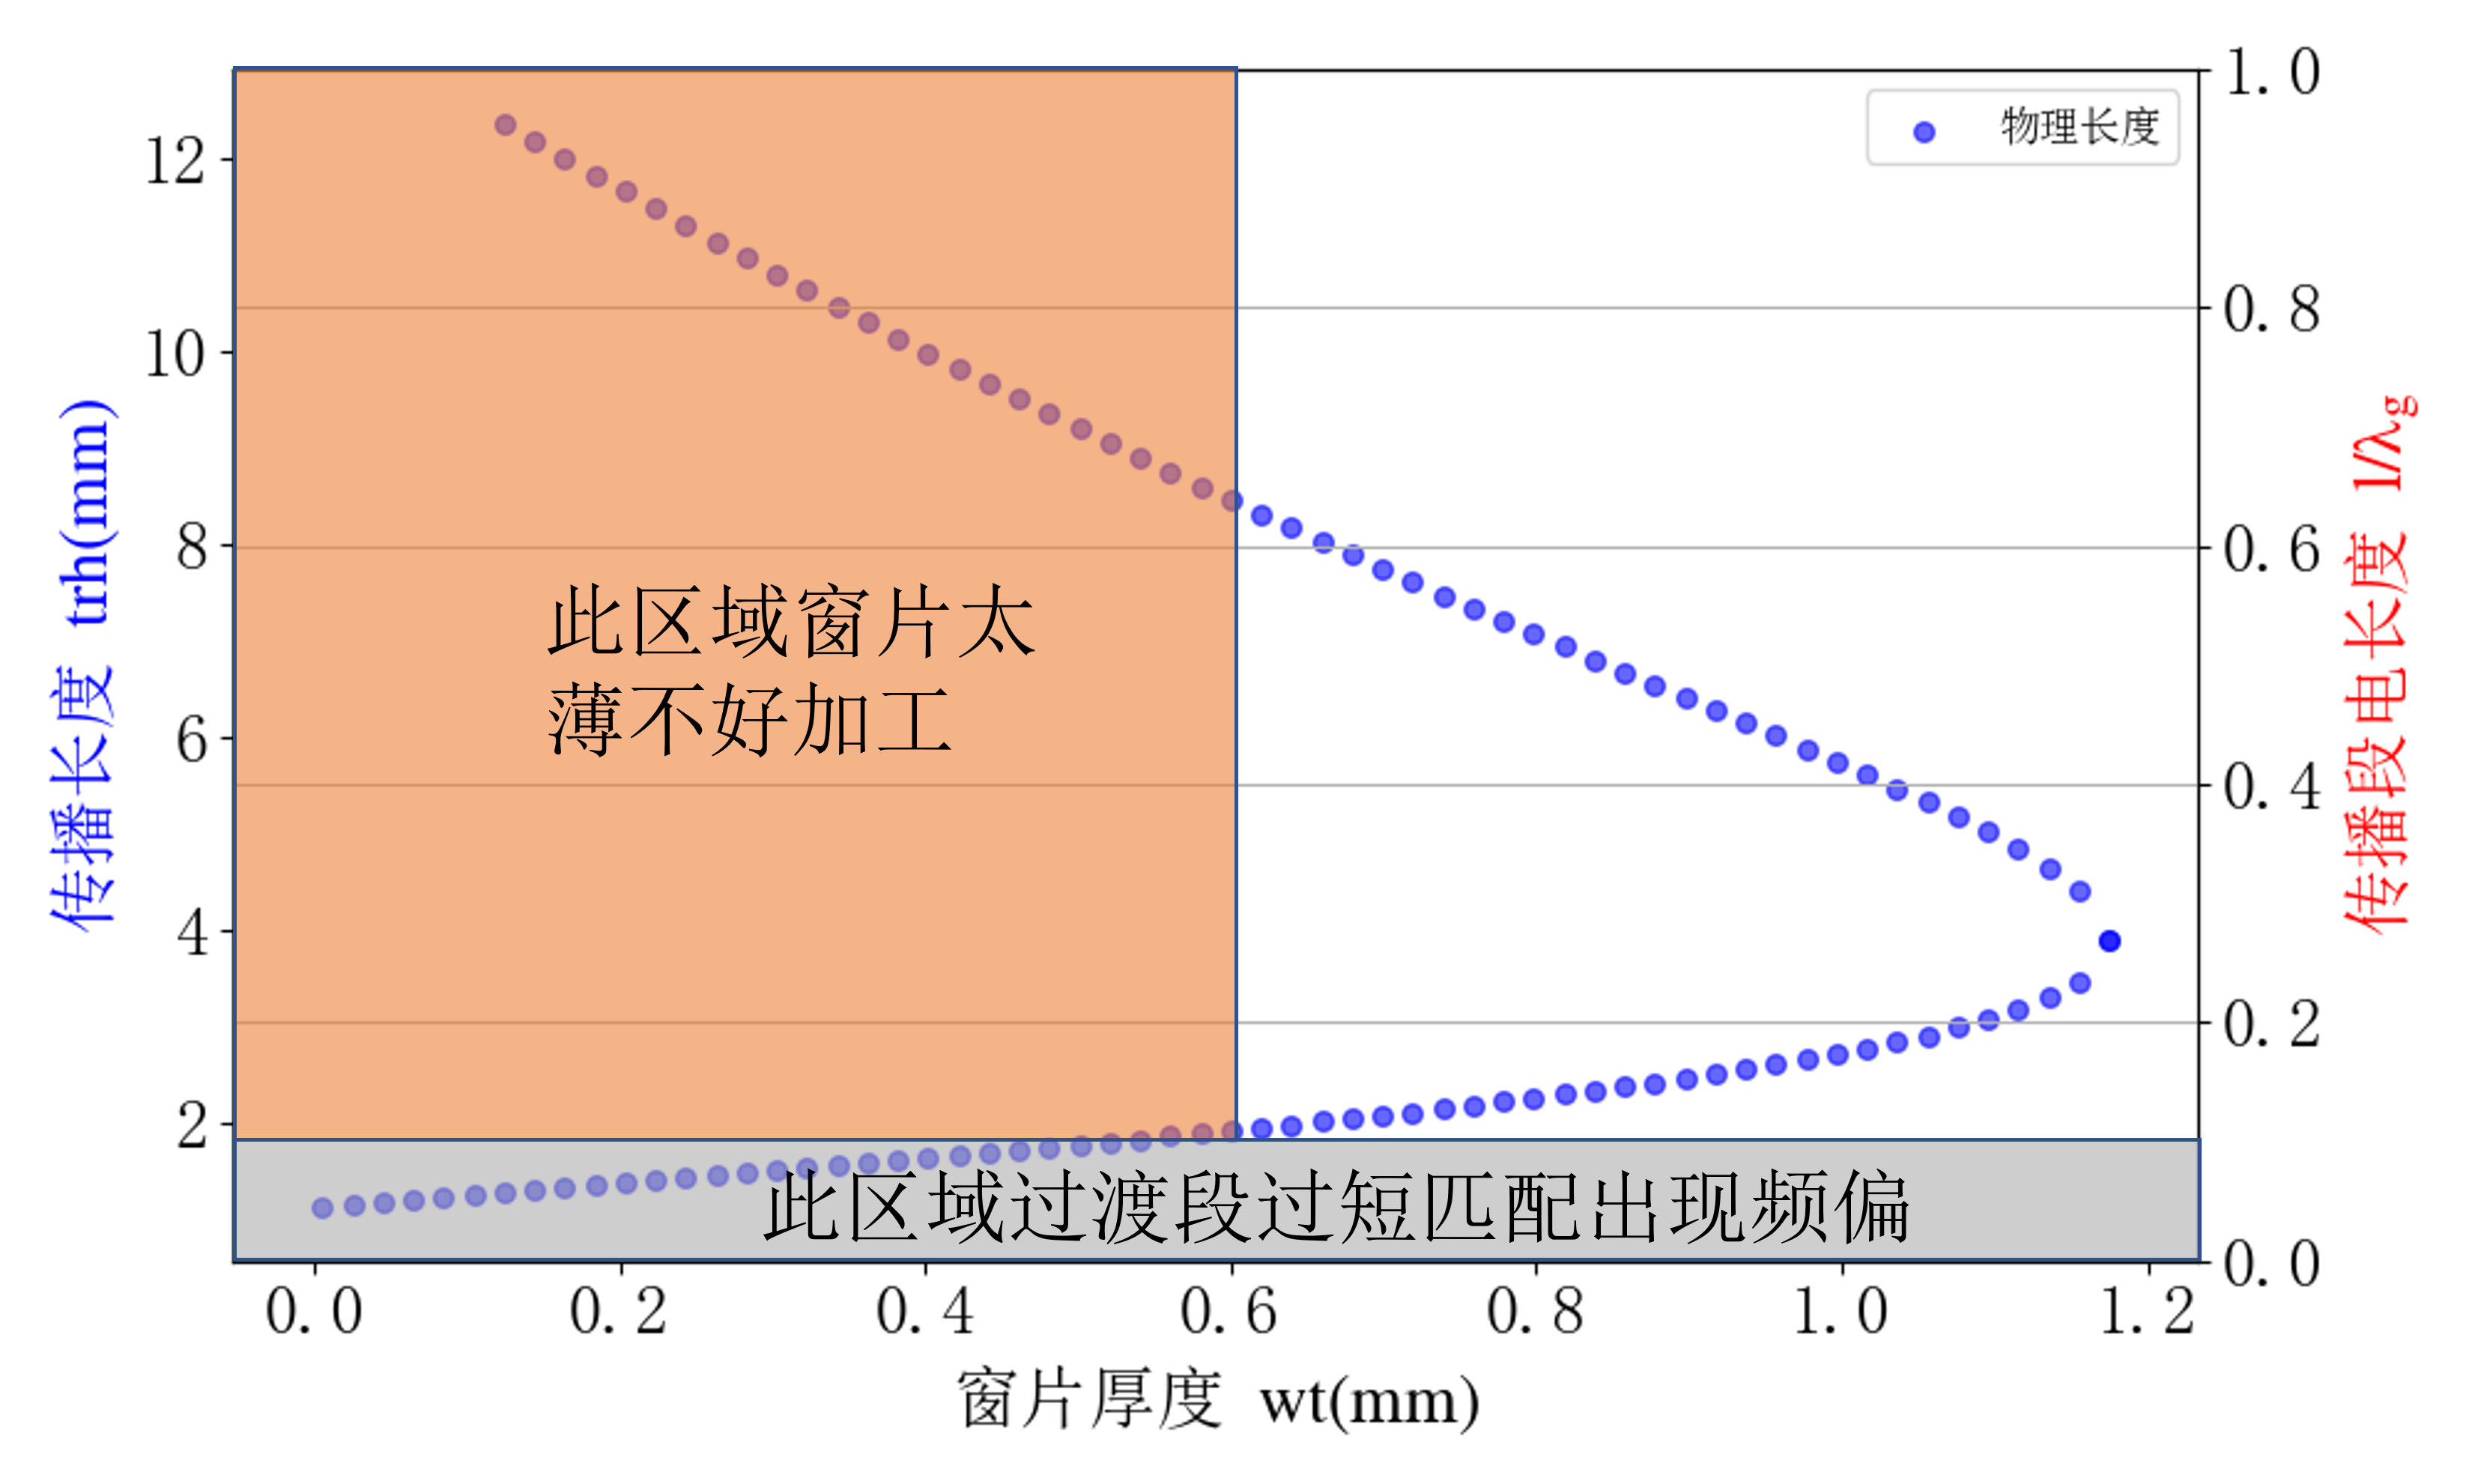
\includegraphics[width=0.45\linewidth]{pic/chapter2/传统盒型窗匹配长度与窗片厚度关系.png}
    \caption{传统盒型窗匹配长度与窗片厚度关系}
    \label{fig:传统盒型窗匹配长度与窗片厚度关系}
\end{figure}

此时选择窗片厚度t=0.62mm的窗,以及匹配段纵向长度l=8.31mm的匹配段,使用上述理论编写Python代码,计算传统盒型窗的匹配频段,并且使用HFSS进行仿真验证。此时的HFSS仿真结果如图\ref{fig:传统盒型窗仿真与计算结果} (b)所示,计算结果如图\ref{fig:传统盒型窗仿真与计算结果} (a)所示,此时的仿真结果与计算结果基本一致,符合预期。HFSS的建模结果如图\ref{fig:传统盒型窗仿真与计算结果} (c)所示。

\begin{figure}[!htbp]
    \small
    \centering
    \begin{tabular}{@{\ }c@{\ }c}
        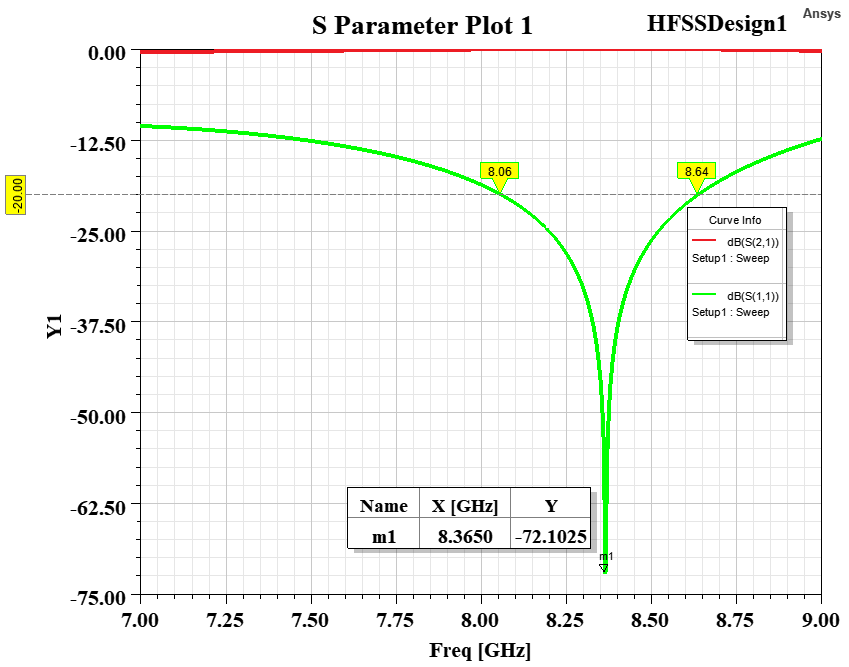
\includegraphics[width=0.35\textwidth]{pic/chapter2/HFSS仿真结果.png} & 
        \hspace{5pt}
        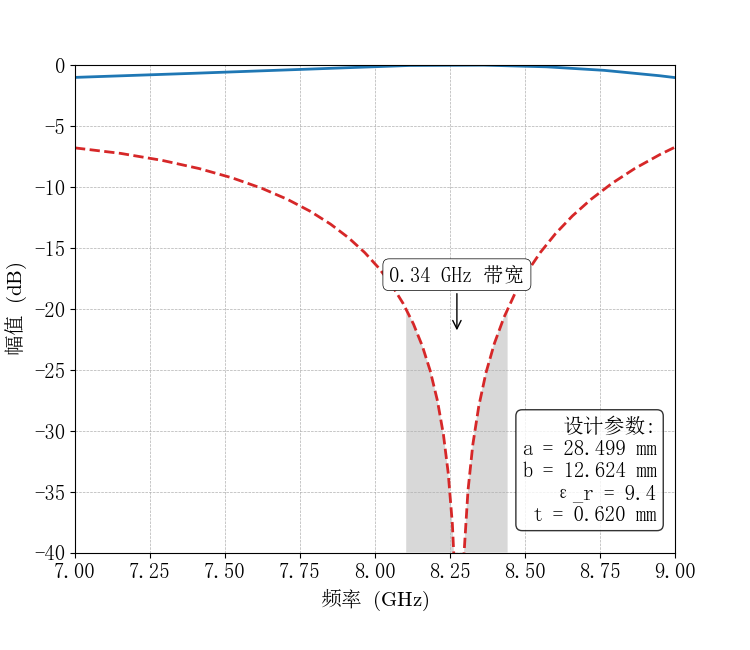
\includegraphics[width=0.35\textwidth]{pic/chapter2/理论计算结果.png}     \\
        \mbox{\small (a)HFSS计算的S参数结果}                                                                               & 
        \mbox{\small (b)理论计算的S参数结果}                                                                                  \\[6bp]
        \multicolumn{2}{c}{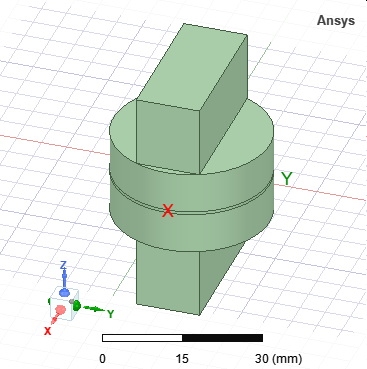
\includegraphics[scale=0.2]{pic/chapter2/HFSS盒型窗建模.png}} \\  % 使用跨列居中
        \multicolumn{2}{c}{\mbox{\small (c) HFSS盒型窗建模}}
    \end{tabular}
    \caption{传统盒型窗仿真与计算结果}
    \label{fig:传统盒型窗仿真与计算结果}
\end{figure}
\section{常见微波窗的损毁机理分析}
微波窗作为真空器件与外界隔离的重要器件,其在使用过程中的可靠性也反映了真空器件整体的可靠性。微波窗在实际应用过程中有可能遭遇极端情况进而产生损毁,其主要的损毁原因为以下陈列的三种情况,分别是:到达环境击穿场强引起击穿、由于电子倍增现象引起损毁以及由于热应力而产生破损,接下来针对这三种情况分别进行进一步的详细分析讨论。
\subsection{到达环境击穿场强引起击穿}
真空器件在工作过程中通常传输着功率较大的电磁波,此时内部的场强较高,当电场的幅值高于环境的击穿场强阈值时便会引发击穿现象。气体的击穿阈值与很多因素有关\citing{lizhigang_2017_spark,zengjie_2017_spark},比如气体的种类、温度、压强等。关于真空器件的击穿阈值,此时可以根据文献\cite{chaiyuanyuan_window_2016}中所给出的公式\ref{eq:击穿阈值估算}进行估算,假设在激励功率为\(P_0\)的情况下器件中的最大电场幅值为\(\left| E_0 \right|\),在到达最大功率容量\(P_{max}\)时候的电场强度为\(E_{max}\),此时\(E_{max}\)即为击穿阈值,它们之间满足以下关系:
\begin{equation}\label{eq:击穿阈值估算}
    \frac{P_0}{\left|E_0\right|^2}=\frac{P_{max}}{\left|E_{max}\right|^2}
\end{equation}
使用此公式时一般来说击穿阈值使用常温常压下空气的击穿场强,即\(\left|E_{max}\right| = 30kV/cm = 3 \times 10^6V/m\),在实际进行应用时可以根据实际的环境条件、器件中所使用的金属或者介质材料种类等其它因素对击穿阈值\(\left|E_{max}\right|\)进行修正。假如最开始仿真软件中使用的激励功率为1W,那么根据以上公式,结合仿真得到的最大场强值和击穿阈值便能初步估算器件的功率容量,方便进行进一步的仿真。
\subsection{电子倍增现象引起击穿}\label{sec:电子倍增现象理论}
在太空中,由于真空器件在运行过程中腔体处于真空状态,除了因为腔体中到达上述最大电场场强阈值进而发生击穿现象的情况之外,由于电子倍增现象进而引发击穿的情况也并不少见。电子倍增现象是指,当电子由于电场等因素的驱使轰击到金属或者介质的表面时,金属或者介质表面被激发出来的电子数目大于入射电子数目的现象。电子倍增现象的示意图可见于图\ref{fig:二次电子发射示意图}中,电子倍增现象一旦被引发,当有电子轰击在波导或者介质的表面上时,很容易雪崩式的在这些表面聚集大量的电子。当这些电子的密度到达一定程度的时候,它们会引发微放电,进而引起器件的击穿或者损坏。
\begin{figure}[!htb]
    \centering
    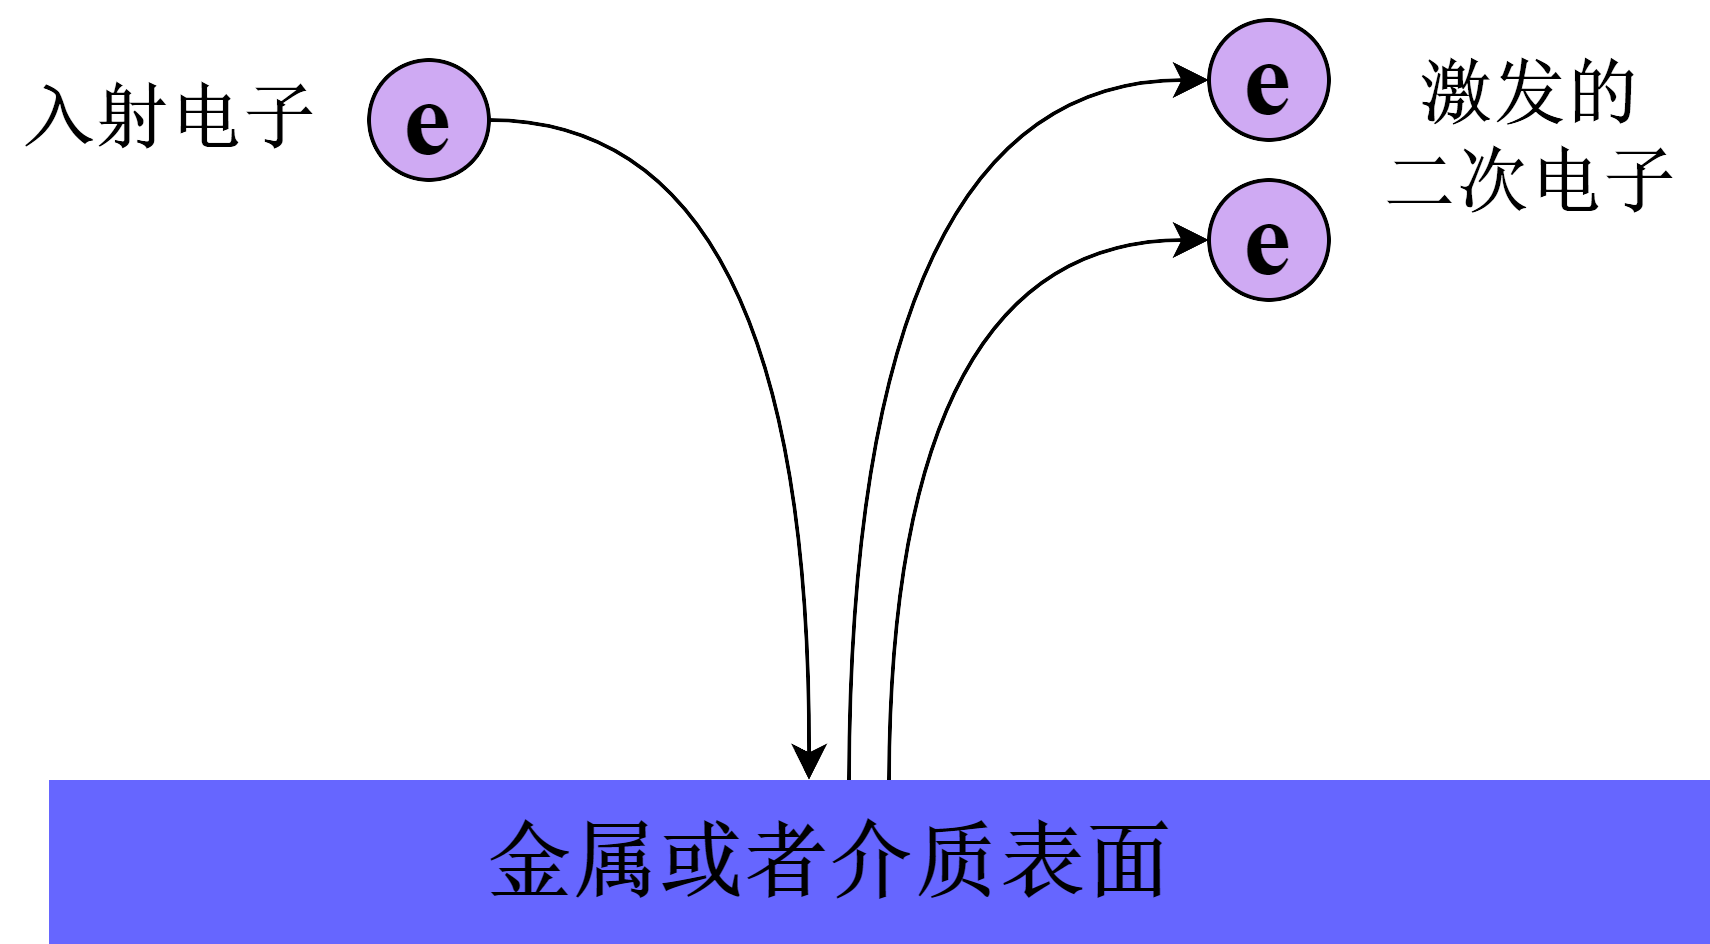
\includegraphics[width=0.5\textwidth]{pic/chapter2/二次电子发射示意图.png}
    \caption{电子倍增现象示意图}
    \label{fig:二次电子发射示意图}
\end{figure}

在研究电子与材料表面相互作用的过程中,特别是探讨二次电子倍增的情形时,Barber\citing{barber_1921_secondary}在1921年提出了一种衡量标准——二次电子产额(SEY)。根据其定义,SEY表示的是单个原始电子撞击某一固体表层之后生成的电子总数。其表达式可以被表示为式子\ref{eq:SEY},式子中的$N_{leave}$的意思是经过入射电子轰击固体材料表面之后离开固体材料表面的电子数目,$N_{primary}$的意思是入射电子的数目:
\begin{equation}\label{eq:SEY}
    \delta = \frac{N_{leave}}{N_{primary}}
\end{equation}

电子倍增是一个随机过程,对于同一种固体材料,当电子轰击到材料表面并且引发电子倍增时,影响SEY的主要因素便是轰击的能量大小($E_p$)与入射角度($\theta$)。一般来说,垂直轰击材料表面的入射电子激发的二次电子数目会比较少,但是斜射入的入射电子激发的二次电子数目会比较多。入射电子的能量必须处于一个特定的能量范围之内才能引起电子倍增效应的产生。如果入射电子的能量过低,会导致电子射入材料表面的深度过浅,也无法让材料内部的电子突破材料的势垒,无法引发电子倍增效应。如果入射电子的能量过高,会导致电子深入材料的深度过深,导致被激发出来的电子深度也过深,进而导致受激发的电子被材料内部消解,无法在材料的表面产生电子倍增。

为了更好地描量化某种材料表面的电子倍增现象的严重程度,提出了材料表面二次电子发射特性的函数关系。为了后续的表述方便,后续本文中提到二次电子发射特性的函数关系将会被简称为二次电子发射曲线。表面二次电子发射特性\citing{jianweifang_lizi_2023}指的是材料表面的SEY与入射电子能量$E_p$之间的函数关系。一个典型的金属表面的二次电子发射特性的函数关系可以被表示如图片\ref{fig:SEY_EP}中所示:
\begin{figure}[!htb]
    \centering
    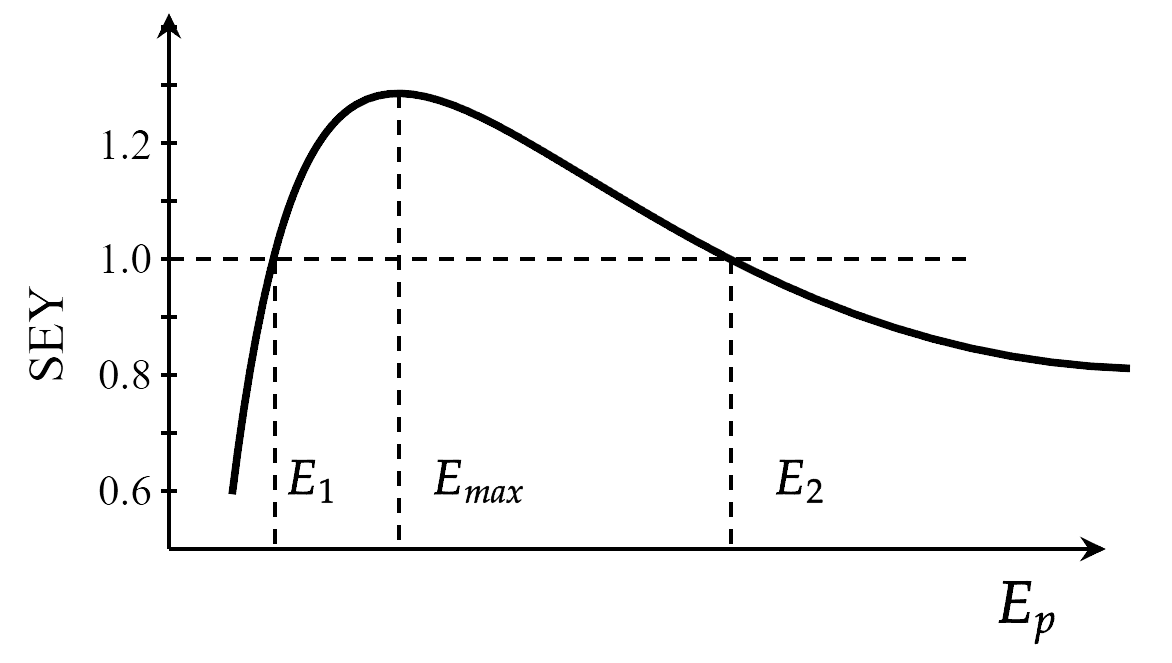
\includegraphics[width=0.5\textwidth]{pic/chapter2/二次电子发射曲线.png}
    \caption{金属的典型的二次电子发射曲线}
    \label{fig:SEY_EP}
\end{figure}

这个曲线在三个特征点处有着各自对应的物理意义,图中的$E_1$表示着入射电子轰击能量从0开始逐渐增大的过程中,SEY首次等于1时的入射电子能量值;$E_{max}$对应着SEY到达最大值时候初始电子能量的值。根据之前分析,再增大入射电子能量SEY值反而会回落,此时的$E_2$值便表示着随着入射能量的继续增大,在SEY值到达最大值之后,再次回落到1时候的入射能量$E_p$的值。

为了准确的描述与预测SEY随着入射能量的变化而产生的变化,有必要建立相关数学物理模型。相关的描述模型有很多,比较有代表性的的模型便是Furman\citing{furman_2002_model}模型和Vaughan\citing{vaughan_1988_multipactor,vaughan_1989_newformula}模型。由于Furman模型针对入射电子轰击到固体材料表面之后的物理过程进行了诸如散射或者被材料吸收等的分类,但是实际上进行实际的测量实验时针对详细的物理过程难以进行实际的观察。为了使用Furman来提高实际拟合精度所付出的代价要远大于直接使用Vaughan模型进行数值拟合。故本文研究的主要模型是Vaughan模型,本文之下将要详细介绍的也是此模型。Vaughan模型是一种唯象模型,其只针对二次电子发射现象进行数据拟合,并未从中提取出更为严谨的物理机理。但是其数据拟合方便并且也比较精准,至今仍在研究二次电子发射现象过程中被广泛使用。

描述SEY的Vaughan模型中的计算公式为:

\begin{equation}\label{eq:SEY_Vaughan}
    \frac{\delta(\theta)}{\delta_{\max}(\theta)} = 
    \begin{cases} 
    \left( \varepsilon e^{1 - \varepsilon} \right)^{0.56} & \text{if } \varepsilon \leq 1 \\
    \left( \varepsilon e^{1 - \varepsilon} \right)^{0.25} & \text{if } 1 < \varepsilon \leq 3.6 \\
    \frac{1.125}{\varepsilon^{0.35}} & \text{if } \varepsilon > 3.6
    \end{cases}
\end{equation}
其中,
$$
\varepsilon = \frac{E_p - E_t}{E_{\max}(\theta) - E_t}
$$

$$
\delta_{\max}(\theta) = \delta_{\max}(0) \left( 1 + k_s \frac{\theta^2}{2\pi} \right)
$$

$$
E_{\max}(\theta) = E_{\max}(0) \left( 1 + k_s \frac{\theta^2}{2\pi} \right)
$$

以上公式中,$E_p$为入射电子能量,$\theta$为入射电子角度,$\delta_{max}$为SEY的最大值,$E_{max}$为$\delta_{max}$所对应的入射电子能量,$E_t$为入射电子截止能量,$k_s$为表面光滑度因子。

为了减小电子倍增现象对器件造成的影响,可以在了解影响材料的SEY影响原因之后,针对性的对器件的结构进行改造进而减小电子倍增现象的产生。例如,不同的固体材料的SEY值不同,可以选择低SEY材料对材料表面进行处理或者使用直接使用材料\citing{ren_2020_multipactor_simulation}对器件进行填充;其次是确保器件的表面光整度以及减少加工过程中\citing{li_2021_novel_multipactor}产生的缝隙,如果材料的表面较为粗糙或者有加工缝隙,会导致斜射到材料表面的概率增加,从而导致产生二次电子倍增现象的概率增加。除了上述所提到的主要影响原因之外,有时候SEY还会遇到诸如材料在空气中受到氧化进而产生性质变化,或者大气压的变化等原因产生影响。
\subsection{由于热应力引起的损毁}
窗片在工作的过程中,会因为其内部的电损耗产热引起窗片内部温度的升高。此时窗片会因为热胀冷缩而导致其发生体积膨胀。如果此时窗片四周的夹具的热膨胀系数与窗片的热膨胀系数\(\alpha\)不一致,就会导致窗片与四周波导或者夹具之间产生挤压进而产生应力,如果应力过大就可能会导致微波窗出现损毁。这种不一致的热膨胀系数还有可能会导致焊接好的窗片与波导间出现缝隙,进而出现窗片气密性下降,从而导致真空器件的真空度下降而损毁整管。

除此之外,如果窗片与四周波导的散热机构没有进行良好设计,在极限功率的工作情况下,窗片表面可能会出现较大的温度差。此时根据论文\cite{lishengming_window_2017}中的描述,当窗片的最大最小温度相差达到\(\Delta T\)时,材料可能会因为温差导致的热应力而而出现裂缝。此时极限温差可以被表述为如下等式\ref{eq:临界温差}所示的形式。其中,\(E\)为材料的弹性模量,\(\sigma_f\)为材料的抗弯强度,\(\alpha\)为热膨胀系数,\(\nu\)为材料的泊松比。
\begin{equation}\label{eq:临界温差}
    \Delta T = \frac{1 - \nu}{E \cdot \alpha} \sigma_f
\end{equation}
故在实际的设计过程中,应该对窗片及其四周的散热机构进行详细的设计,尽量防止窗片的最大最小温度差过大,避免材料因为的热应力过大从而出现裂隙。

\section{本章小结}
本小节首先介绍了微波射频中常用的等效电路分析概念,并且对脊波导的常用工作参数进行了详细的分析。之后对传统结构的盒型窗进行了详细的理论分析,并且在分析的最后使用了HFSS对理论分析的结果进行了检验,说明了盒型窗理论分析部分的正确性。最后针对微波窗常见的损毁机理分为三类,分别是到达击穿场强遭到击穿,由于二次电子倍增而引起损毁,由于热应力过大而导致的损毁。并且给出了二次电子倍增现象的相关理论分析以及避免窗片损毁所引入的材料的极限温差。

\chapter{6-11GHz 宽频带脊波导窗的设计}
\section{引言}
正如前文所说,在真空管中,窗片是其中非常重要的组成部件。窗片需要在指定的频带内进行匹配,并确保适当的机械强度。这保证了频段内信号能够在真空管与外界之间在指定频段之内正常导通。同时,这也维持了真空管内的真空度。

在前面\ref{sec:PillBoxTheory}中提到的传统结构的盒型窗在许多方面上存在局限性。首先从加工层面来说,因为圆形窗片的半径与圆柱形波导的直径相同,如果想要固定介质窗片,那么就必须从侧面对窗片进行焊接。侧面焊接的气密性与窗片的厚度有关,如果窗片太薄,那么在焊接的过程中就会出现不稳定性,并且窗片的机械强度也会受到影响,过薄的窗片很容易出现打火击穿或者内外压差进而碎裂的情况。观察不等式\ref{eq:Delta}并且结合等式\ref{eq:B_d}可以发现,想要特征方程\ref{eq:B-C-simplify2}有解,那么对于窗片的厚度$t$的取值范围有:
\begin{equation}\label{eq:t_constraints}
    0 < t < \frac{\sqrt{\frac{1}{k^2}+4k^2(1+B_{T}^2)^2-2(1-2B_{T}^2)}}{(\varepsilon_{d}-1)(\omega / c)(\lambda_{gc} / \lambda)}
\end{equation}
传统盒型窗的特征方程说明了,为了确保传统薄窗片盒型窗的正常匹配,窗片的厚度$t$必须小于一个阈值,过厚的窗片便不能应用原先的等式\ref{eq:B_d}进行等效电路进而进行计算。

其次,根据之前\ref{sec:PillBoxTheory}中提到的,传统模式的盒型窗的单侧匹配电长度不能低于0.1倍电长度,因为盒型窗需要两端匹配段,那么可以得到盒型窗匹配段连带窗片部分的电长度不会低于0.2倍电长度。这一点难以保证盒型窗在实际进行匹配时候的结构紧凑性。

最后,根据文献\cite{huxiongli_bandwidth_pill},传统意义上的盒型窗的相对带宽最宽可以做到15\% 到20\% 。如果想要进一步的提升盒型窗的带宽,只能对其结构进行相应的改进,例如将窗片的厚度进行进一步的削减,这一步骤可能会影响窗片的机械结构强度与窗片整体结构的气密性。

并且在现阶段,除了传统薄窗片盒型窗之外,窗片的宽带宽实现方案结构不够紧凑,这影响了真空器件的小型化进程。此外,这些方案也面临加工焊接的难题,这一点直接影响了器件的加工与制作。

所以需要一种微波窗的设计方案,它应使微波窗具有宽匹配频带和紧凑结构。此外,该方案还需便于进行窗片的进一步加工处理。本章节将利用脊波导的主模带宽宽的特性,设计一种宽频带脊波导窗。

\section{新型脊波导窗的结构设计}
为了解决盒型窗带宽与匹配结构复杂度之间的矛盾,以及常见的宽带宽窗片解决方案造成的较难以焊接加工或者设计的相关问题。现在对原先的盒型窗片的结构进行进一步的改良,获得一种新型的以脊波导为传输波导,并且以圆形窗片为输入窗片,以圆角矩形为脊波导到窗片之间的过渡段的新型的宽带宽窗。
本次设计的波导窗必须满足以下设计要求:
\begin{enumerate}
    \item 窗片在6-11GHz之内,满足$S_{11}<-20dB$的匹配要求(相对带宽58\%)。
    \item 结构结构紧凑,方便器件的小型化。
    \item 窗片几何结构较为简单,方便后续的加工与焊接。
\end{enumerate}

由于相同频段之下,脊波导相比于同等频段的矩形波导结构更加紧凑,主模带宽更宽。此时考虑功率容量的相关问题,双脊波导的功率容量比单脊波导的功率容量更大,故选择双脊波导作为窗片的波导输能结构。结合小节\ref{subsec:DoubleRidgeTheory}里面的关于双脊波导理论研究,现在初步确定双脊波导的几何参数参数如下:$a=20mm, b=10mm, d=5mm, s=4mm $,具体的脊波导横截面如图\ref{fig:6-11GHzDRW}所示:
\begin{figure}[!htb]
    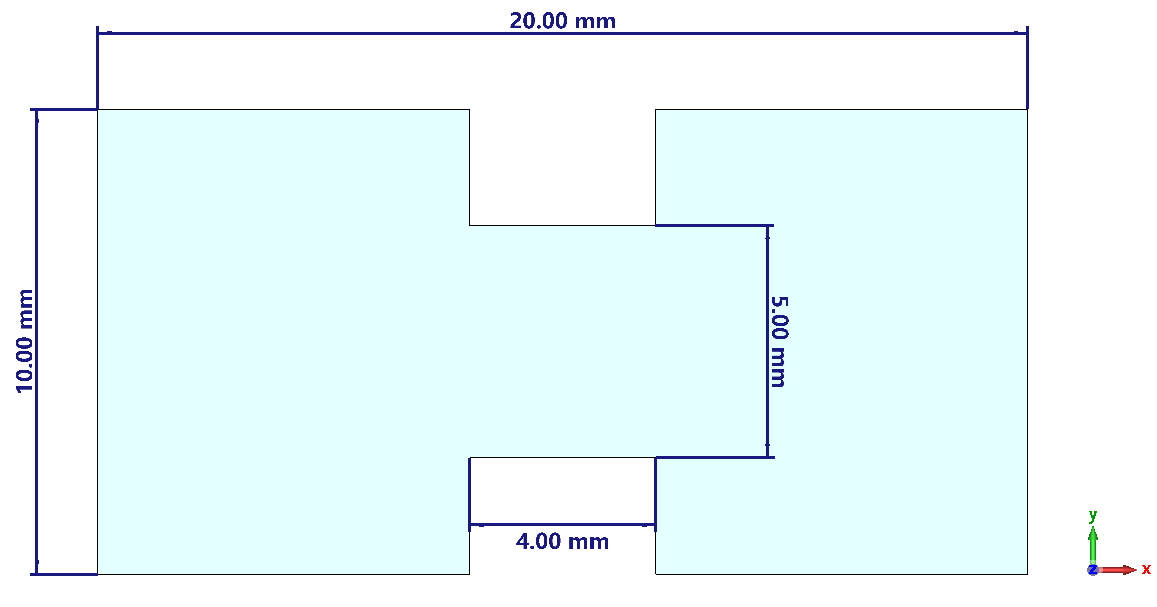
\includegraphics[width=0.7\linewidth]{pic/chapter3/6-11GHzDRW.png}
    \caption{输入窗脊波导几何参数选取}
    \label{fig:6-11GHzDRW}
\end{figure}

很明显,这个脊波导的几何参数满足式子\ref{eq:DRW_constraints}的限制条件,此时可以通过简化式子\ref{eq:DRW_closed}计算双脊波导的截止频率进行计算,得到的计算结果为$f_c$=5.85GHz。此时截止频率小于所需带宽的下限,表明此时选取的脊波导几何参数满足要求。现在使用CST对脊波导的真实截止频率以及直通情况下的S参数进行仿真,得到如图\ref{fig:脊波导初步仿真}的结果。根据图\ref{fig:脊波导初步仿真} (a)结果显示,脊波导的截止频率为$f_c=5.84GHz$,与式子\ref{eq:DRW_closed}的计算结果基本一致。根据图\ref{fig:脊波导初步仿真} (b)显示,此时的双脊波导在要求的频段6-11GHz之内$S_{11}<25dB$,满足匹配要求。

\begin{figure}[!htb]
    \small
    \centering
    \begin{tabular}{@{\ }c@{\ }c}
        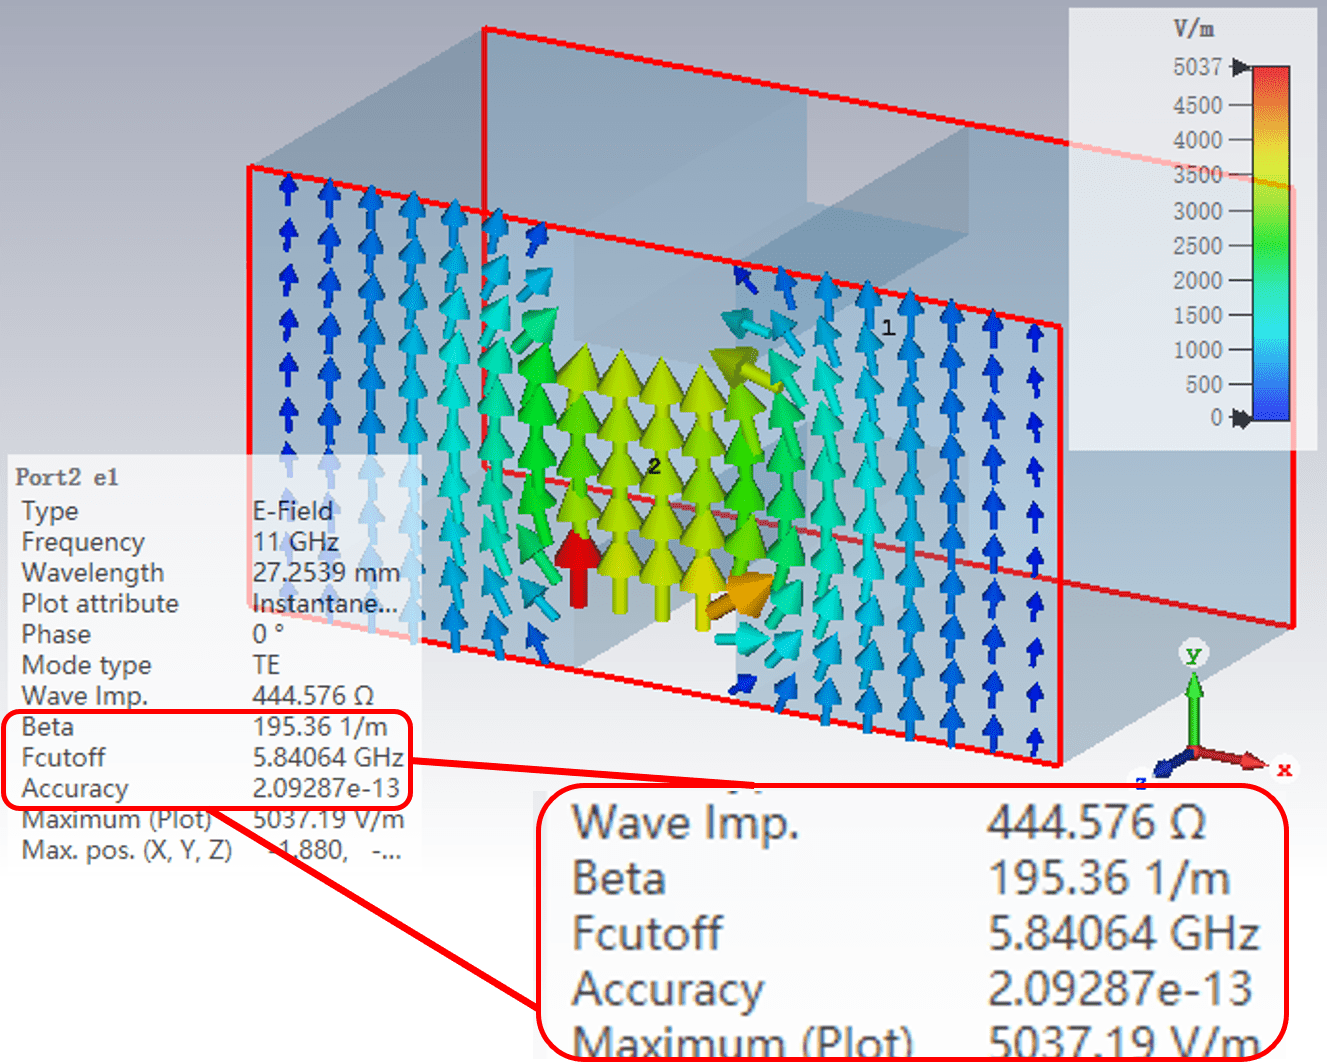
\includegraphics[width=0.45\textwidth]{pic/chapter3/脊波导初步仿真.png} & 
        \hspace{5pt}
        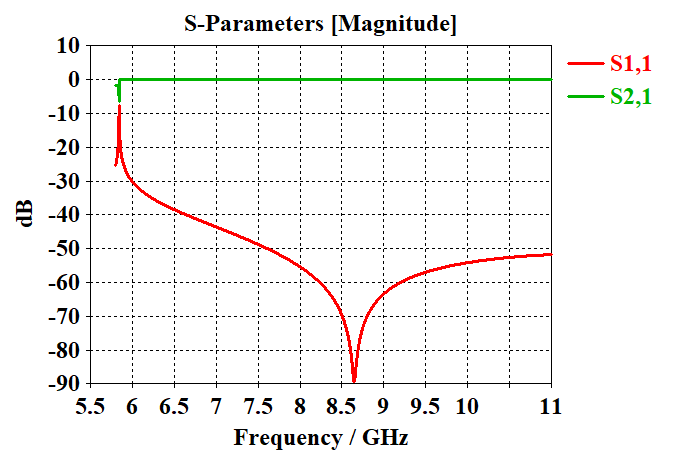
\includegraphics[width=0.45\textwidth]{pic/chapter3/输入窗脊波导S曲线.png}     \\
        \mbox{\small (a)脊波导截止频率仿真}                                                                               & 
        \mbox{\small (b)脊波导S曲线仿真}                                                                                  \\
    \end{tabular}
    \caption{脊波导初步仿真}
    \label{fig:脊波导初步仿真}
\end{figure}

\section{脊波导窗的材料选择}
接下来选取脊波导圆形窗片的材料,根据文章\cite{han_sapphire_2011}里面对窗片材料的论述,蓝宝石的特性包括低介电损耗和高机械强度,使其能够制造出0.1毫米厚的精细层而不会因为管内外压差而产生破损;由于它是致密无孔的晶体材料,内部结构均匀,所以在高功率操作环境下不易发生熔解破坏。此外,它还能应对焊接和真空脱气过程中的高温,当实现大规模生产时,成本控制良好,且环保方面的问题较少。因为蓝宝石的上述优点,本文选取蓝宝石作为窗片的材料。根据材料\cite{thumm_2020_State}所示,将蓝宝石的相对电介质常数设定为$\varepsilon_r=9.4$,损耗角正切被设定为$\tan \delta = 0.0004$。


\section{脊波导窗的结构设计}
经过计算仿真,最终确定脊波导窗片的整体结构为图\ref{fig:脊波导窗的整体结构}所示。
\begin{figure}[!htb]
    \centering
    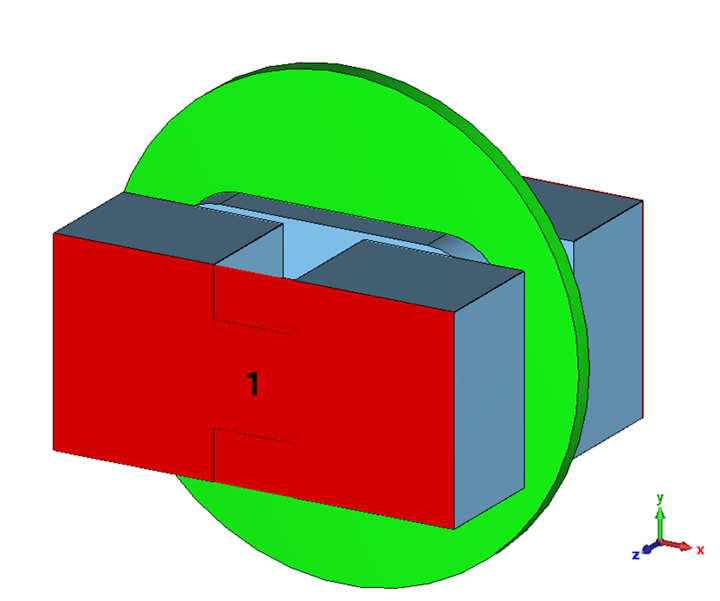
\includegraphics[width=0.45\linewidth]{pic/chapter3/输入窗的总体视图.png}
    \caption{脊波导窗的整体结构}
    \label{fig:脊波导窗的整体结构}
\end{figure}

为了方便设计加工与焊接,窗片被设置为圆形窗片。为了减少匹配段的长度,窗片与脊波导之间的过渡部分被设计为倒圆角的矩形过渡段。其中对过渡部分倒圆角不仅是为了降低过渡段的最大场强,提升窗片的功率容量,防止窗片被击穿;另一方面也方便了之后对过渡段部分的加工。

各个部分的详细尺寸被记载于图\ref{fig:窗片与过渡段的尺寸}中。其中\ref{fig:窗片与过渡段的尺寸} (a) 展示了窗片的直径为22.98mm。图片\ref{fig:窗片与过渡段的尺寸} (b)展示了圆窗片与脊波导之间的圆角矩形过渡段的具体尺寸,其长边为16.03mm,短边为10.61mm,四个角均倒圆角,倒圆角的半径为2.85mm。结构具体的纵向长度如图\ref{fig:窗片与过渡段的尺寸} (c)所示,圆角矩形过渡段的纵向长度为1.69mm,窗片的厚度为0.91mm。

\begin{figure}[!htbp]
    \small
    \centering
    \begin{tabular}{@{\ }c@{\ }c}
        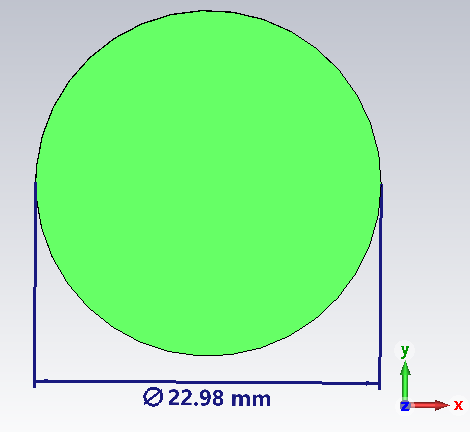
\includegraphics[width=0.25\textwidth]{pic/chapter3/圆形窗片视图.png} & 
        \hspace{5pt}
        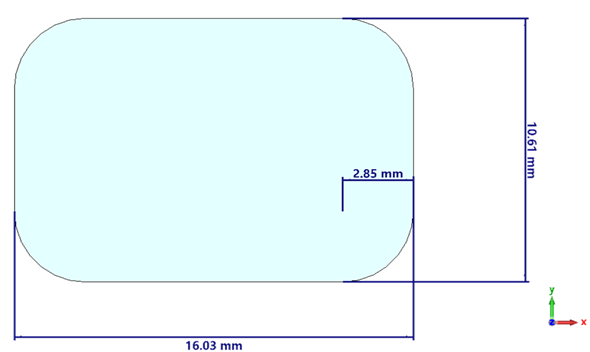
\includegraphics[width=0.45\textwidth]{pic/chapter3/圆角矩形视图.png}     \\
        \mbox{\small (a)圆形窗片视图}                                                                               & 
        \mbox{\small (b)圆角矩形视图}                                                                                  \\[6bp]
        \multicolumn{2}{c}{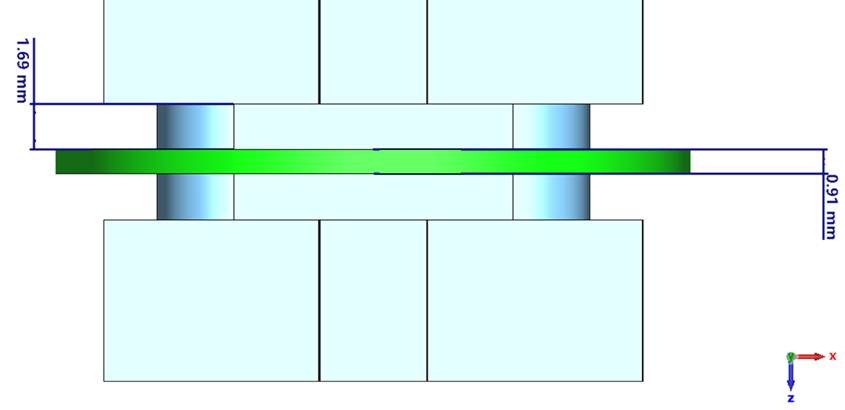
\includegraphics[scale=0.21]{pic/chapter3/纵向长度视图.png}} \\  % 使用跨列居中
        \multicolumn{2}{c}{\mbox{\small (c)纵向长度}}
    \end{tabular}
    \caption{窗片与过渡段的尺寸}
    \label{fig:窗片与过渡段的尺寸}
\end{figure}

此时对脊波导窗的过渡段部分电长度进行分析,并与传统盒型窗进行对比。根据上文的分析,为了满足盒型窗窗片两侧过渡部分能够被等效为传输线的物理模型这一目的,传统盒型窗的匹配段部分不得小于0.1倍电长度。如果不满足这一要求就会因为无法被等效为传输线模型进而导致设计的匹配点出现频偏。此时新型盒型窗的过渡段可以被视作工作在$TE_{01}$下的长边为16.03mm,短边为10.61mm矩形波导,计算其在$10GHz$的工作波长为$\lambda_{gRec}=\lambda / \sqrt{1-(\lambda / \lambda_c)^2}=85.06mm$,匹配部分的电长度小于0.1倍电长度,相比于传统盒型窗的匹配部分的电长度更短,故新型窗片的匹配部分结构更加紧凑。

\section{脊波导窗的S参数仿真}
此时对原先参数的脊波导窗在CST里面进行建模,并且使用频域求解器在匹配频段内进行仿真,计算得到窗片的S参数如图\ref{fig:输入窗的S参数}所示:

\begin{figure}[!htb]
    \centering
    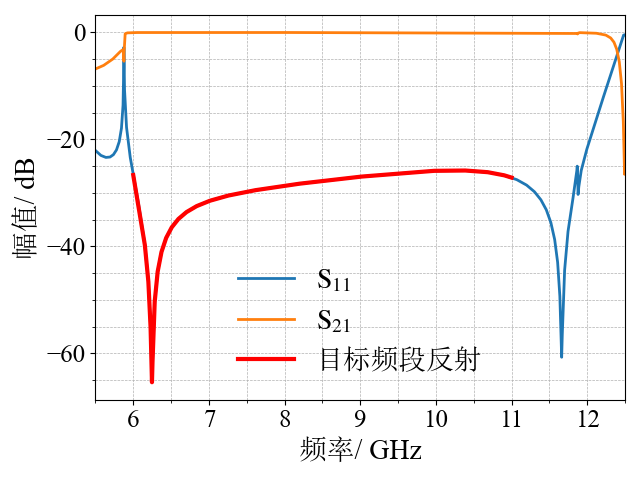
\includegraphics[width=0.5\linewidth]{pic/chapter3/脊波导窗S参数.png}
    \caption{输入窗的S参数}
    \label{fig:输入窗的S参数}
\end{figure}
对窗片的S参数进行考察,发现其反射系数$S_{11}$在要求的频段6-11GHz之内小于-20dB,满足匹配要求。此时结合图片可以得到满足反射系数$S_{11}$<-20的频带范围为6-11GHz,此时计算其相对带宽为62.9 \%。

\subsection{脊波导窗的参数敏感度分析}\label{subsec:脊波导窗的参数敏感度分析}
为了方便对后续的窗片加工进行误差方面进行指导,了解反射系数\(S_{11}\)与参数之间的敏感度关系。有必要进行反射系数与窗片参数敏感度相关的仿真。

在进行初步的敏感度分析仿真之后,将最为敏感的几个参数筛选出来在此进行讨论。在之后的加工过程中,确保这几个参数所相关的几何参数在之后的加工过程中更应该格外注意精度相关的控制。本次仿真能够通过参数敏感度检验的前提是,参数在范围内变化时反射系数在频段6-11GHz内始终满足\(S_{11}<-20dB\)。

首先针对过渡段的参数进行相关的扰动与扫参来进行参数敏感度分析,具体的扫参结果如图\ref{fig:X频段脊波导窗过渡段参数敏感度分析}所示。具体的扫参结果如图\ref{fig:X频段脊波导窗过渡段参数敏感度分析}所示。根据图\ref{fig:X频段脊波导窗过渡段参数敏感度分析}(a)的仿真结果,过渡段长度在加工过程中应保持在15.85mm<ta<16.55mm 范围内。图\ref{fig:X频段脊波导窗过渡段参数敏感度分析}(b)显示,过渡段宽度应控制在9.8mm<tb<11.35mm 之间。最后,依据图\ref{fig:X频段脊波导窗过渡段参数敏感度分析}(c),过渡段厚度的理想范围是1.35mm<trh<1.82mm 。

根据上述分析,此时关于过渡段波导的厚度的影响对反射系数的影响最大,在进行加工的过程中应该对其进行更加严格的把控。
\begin{figure}[!htbp]
    \small
    \centering
    \begin{tabular}{@{\ }c@{\ }c}
        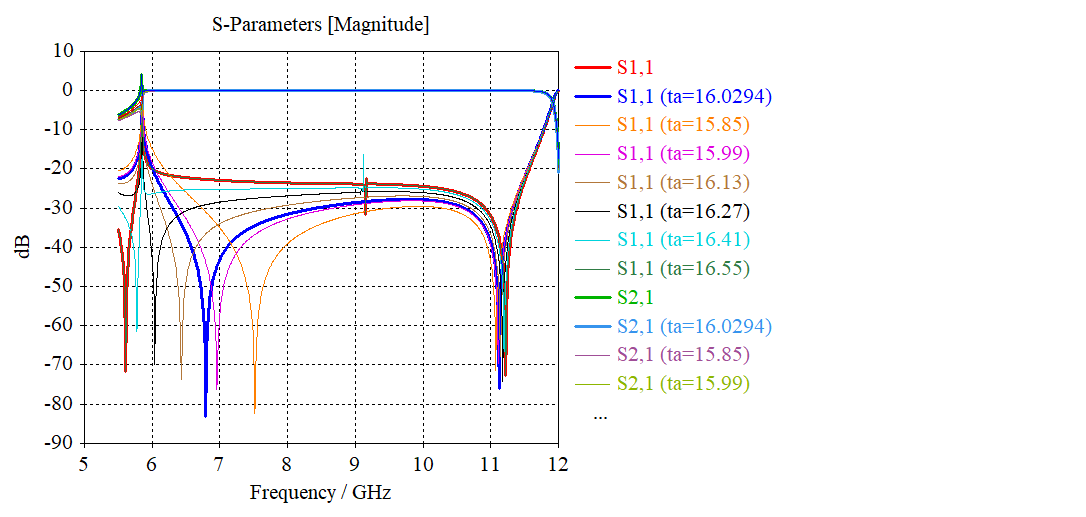
\includegraphics[width=0.45\textwidth]{pic/chapter3/脊波导窗过渡段长度ta扫参.png} & 
        \hspace{5pt}
        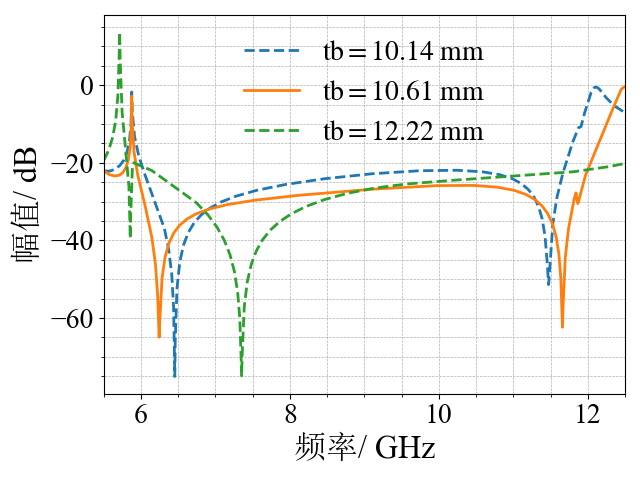
\includegraphics[width=0.45\textwidth]{pic/chapter3/脊波导窗过渡段宽度tb扫参.png}     \\
        \mbox{\small (a) 过渡段长度ta敏感度分析}                                                                               & 
        \mbox{\small (b) 过渡段长度tb敏感度分析}                                                                                  \\[6bp]
        \multicolumn{2}{c}{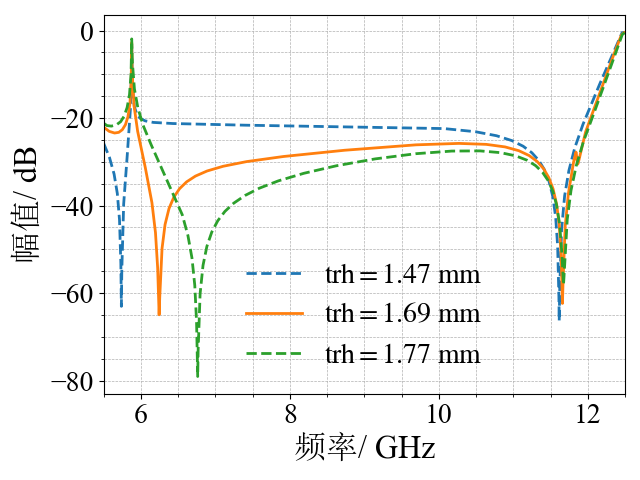
\includegraphics[width=0.55\textwidth]{pic/chapter3/脊波导窗过渡段厚度trh扫参.png}} \\  % 使用跨列居中
        \multicolumn{2}{c}{\mbox{\small (c) 过渡段厚度trh敏感度分析}}
    \end{tabular}
    \caption{6-11GHz脊波导窗过渡段参数敏感度分析}
    \label{fig:X频段脊波导窗过渡段参数敏感度分析}
\end{figure}

在进行了敏感度分析之后,需要对窗片相关的几何参量的敏感度进行分析。此时窗片半径\(wr\)应该在范围\(41.2mm<wr<43.2mm\)之内,窗片的厚度\(wt\)应该满足\(5.55mm<wt<6.67mm\)。在参数位于以上的范围之内时,才能够确保窗片的设计符合性能要求。此时可以看出,无论是窗片的半径还是厚度都对窗片的S参数产生非常明显的影响,在加工过程中,应该对窗片在这两个指标上的控制更加严格。
\begin{figure}[!htb]
    \small
    \centering
    \begin{tabular}{@{\ }c@{\ }c}
        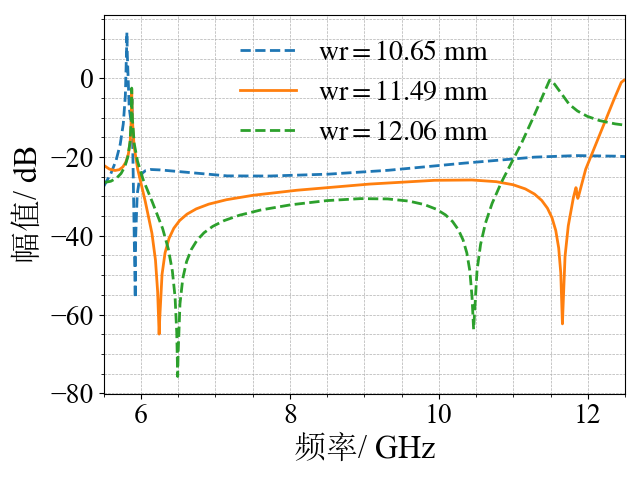
\includegraphics[width=0.35\textwidth]{pic/chapter3/窗片半径wr扫参.png} & 
        \hspace{5pt}
        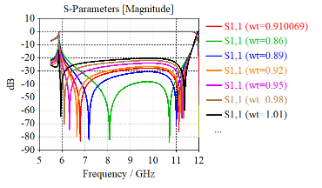
\includegraphics[width=0.35\textwidth]{pic/chapter3/窗片厚度wt扫参.png}     \\
        \mbox{\small (a)窗片半径wr敏感度分析}                                                                               & 
        \mbox{\small (b)窗片厚度wt敏感度分析}                                                                                  \\
    \end{tabular}
    \caption{6-11GHz脊波导窗窗片参数敏感度分析}
    \label{fig:X频段脊波导窗窗片参数敏感度分析}
\end{figure}

\section{计算脊波导窗功率容量}
为了探究输入窗的适用范围,有必要对脊波导窗的功率容量进行分析。微波窗通常在电场强度最强处出现击穿,并且在扫参时候发现,在同一匹配频段内,低频点的电场强度更强。根据这些结论,现在对脊波导窗的在需要频段的低频点(6GHz)处的电场场强进行仿真,电场强度分布如图\ref{fig:X频段脊波导窗低频点场强仿真} (a)所示,此时在使用CST的有效值为1W的波导端口进行激励时,最大电场幅值为\(17773V/m\)。为了方便进一步地分析,需要找到最大场强所在位置,其最大场强位于脊波导的脊与过渡段的交界处,具体位置如\ref{fig:X频段脊波导窗低频点场强仿真} (b)所示。
\begin{figure}[!htb]
    \small
    \centering
    \begin{tabular}{@{\ }c@{\ }c}
        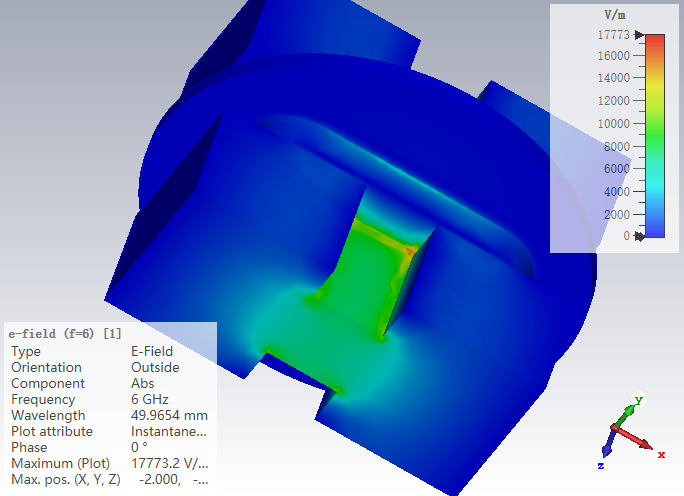
\includegraphics[width=0.4\textwidth]{pic/chapter3/X频段等效1W最大场强.png} & 
        \hspace{5pt}
        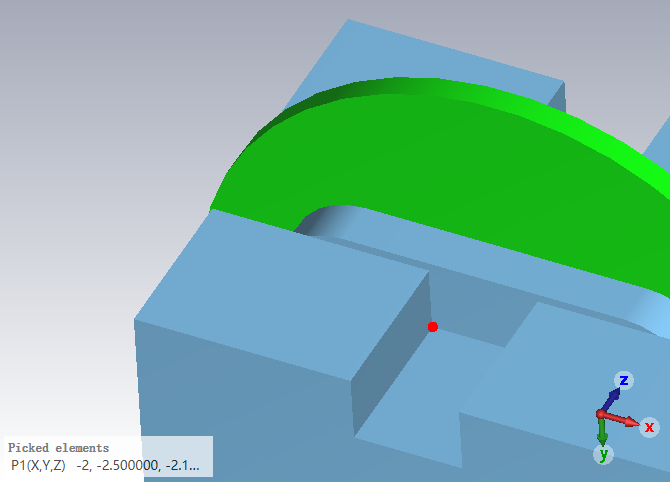
\includegraphics[width=0.4\textwidth]{pic/chapter3/X频段最大场强出现位置.png}     \\
        \mbox{\small (a)X频段脊波导窗电场分布}                                                                               & 
        \mbox{\small (b) X频段脊波导窗最大电场出现位置}                                                                                  \\
    \end{tabular}
    \caption{6-11GHz脊波导窗低频点场强仿真}
    \label{fig:X频段脊波导窗低频点场强仿真}
\end{figure}

完成最大场强所在位置的标定之后,可以开始对脊波导窗功率容量进行进一步的分析。此时使用第二章中的计算公式\ref{eq:击穿阈值估算}进行初步分析,因为CST使用的默认激励功率为有效值1W,此时相当于\(P_{1}=0.5W\),根据仿真结果,此时\(E_1 = 17773V/m\),使用空气的击穿场强\(3 \times 10^6V/m\)作为击穿最大电场场强值。综上所述,此时估算的最大功率容量为\(P_{max}=14.2kW\)。但是为了确保估算结果的准确性,本文采用了两种不同的仿真方式对估算结果的功率容量进行对照。
\subsection{使用最大场强法计算脊波导窗的功率容量}\label{subsec:X最大场强功率容量}
最大场强法主要是通过对端口的输入功率进行扫参,当仿真器件的最大场强到达击穿阈值时便判定为击穿。根据经验值,室温常压下的空气的击穿场强是30kV/cm。故在进行仿真的时候,如果瞬时电场的最大场强值达到30kV/cm的空气击穿场强时便被视为击穿。但是在实际的窗片加工的过程中,窗片的实际功率容量并不全与这个方法所计算出来的功率容量相一致,实际情况下由于环境的不同,空气的击穿场强也会随着产生变化。故此方法得到的功率容量的值仅供参考,在实际应用过程中需要针对最大场强法进行计算的功率容量进行修正。

此时在低频点(6GHz) 处设定电场监视器,并且使用后处理模板提取电场监视器的电场场强的最大值作为跟根据仿真结果\ref{fig:输入窗最大场强结果}显示,在馈入端口的功率到达3.1kW的时候,窗片内的最大场强达到30kV/cm。故使用最大场强法进行分析时,窗片的功率容量应该在3.1kW。
\begin{figure}[!htb]
    \centering
    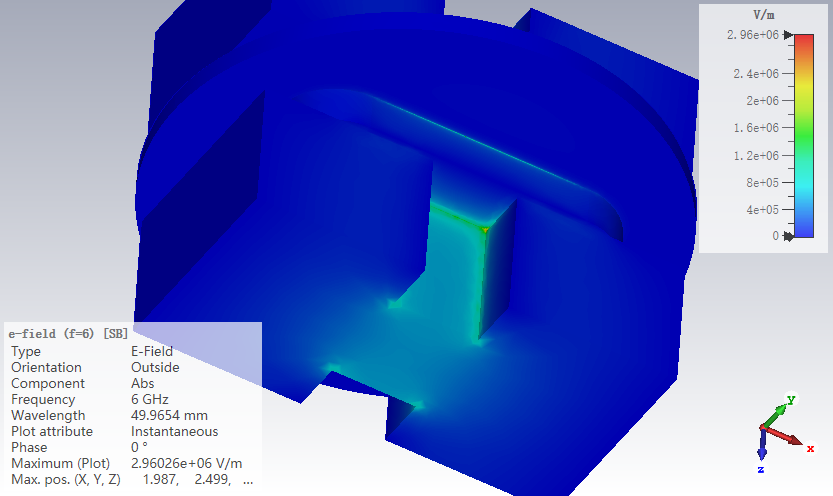
\includegraphics[width=0.5\linewidth]{pic/chapter3/X频段最大功率场强.png}
    \caption{输入窗最大场强结果}
    \label{fig:输入窗最大场强结果}
\end{figure}

\subsection{使用二次电子倍增计算脊波导窗的功率容量}\label{subsec:X二次电子倍增功率容量}
正如前面小节\ref{sec:电子倍增现象理论}中所说,电子倍增现象是影响真空器件在太空中的功率容量的重要原因。为了更加完全验证器件的功率容量,除了前面的最大场强分析法,有必要使用二次电子倍增理论对器件的功率容量进行进一步的分析。

前面已经使用CST针对器件的S参数进行了仿真并且已经验明原先的器件的S参数符合设计要求,本次将使用CST中的SPARK3D模块进行先验仿真,并使用PIC模块对原先的器件进行基于二次电子倍增的详细功率容量仿真。

\subsubsection{铜与蓝宝石的材料二次电子曲线设置}
由于关于二次电子产额和入射电子能量相关曲线有许多种不同的测量方法,每种测量方法之间的结果与精度\citing{guanghuimiao_2018_measurement}相差较大,并且不同的二次电子发射曲线所带来的结果也不尽相同,故本文在引用二次电子发射曲线时尽量从多篇文章中找到曲线并且对参数进行综合考量后再进行分析。

首先根据文献\cite{valizadeh_2014_wja}能获得关于在Vaughan模型中中入射电子能量从80到1000电子伏特时候的二次电子发射曲线,的铜的二次电子发射曲线的关键参数分别为$\delta_{max}=1.9, E_{max}=300 eV$;在文章\cite{bojko_2020_see}中测量了入射电子能量从60到3000电子伏特的铜的二次电子发射曲线,其关键参数为$\delta_{max}=1.6, E_{max}=352 eV$;文章\cite{jianweifang_lizi_2023}中测量了入射电子能量从50到1000电子伏特的铜的二次电子发射曲线,其关键参数为$\delta_{max}=1.76, E_{max}=250 eV$。从这些论文中综合他们所测量的二次电子发射曲线,可以得到使用Vaughan模型的无氧铜的二次电子发射曲线中的关键值为:$\delta_{max}=1.9, E_{max}=300 eV$,并且设置CST中的二次电子发射曲线的入射电子能量区间为50到1000电子伏特,入射方式为垂直入射,其余参数保持默认。

此时根据文献\cite{suharyanto_2006_secondary}测量了入射电子能量从0.5-5keV的蓝宝石二次电子发射系数,此时相关的关键参数为$\delta_{max}=7.91, E_{max}=0.99keV$;文献\cite{chvyreva_2014_experimental}展示了蓝宝石的二次电子发射曲线关键参数为$\delta_{max}=7.8, E_{max}=0.65keV$。本文后续使用的参数为$\delta_{max}=7.91, E_{max}=0.65keV$,CST中设置二次电子发射曲线的入射电子能量区间为50到5000电子伏特,入射方式为垂直入射,其余参数保持默认。本文后续将使用这些文献中所展示的关键参数,结合前文中所示的Vaughan模型\ref{eq:SEY_Vaughan}对器件的二次电子发射情况进行仿真,设置完成后的曲线如图\ref{fig:X波段材料二次电子发射特性}所示。
\begin{figure}[!htb]
    \small
    \centering
    \begin{tabular}{@{\ }c@{\ }c}
        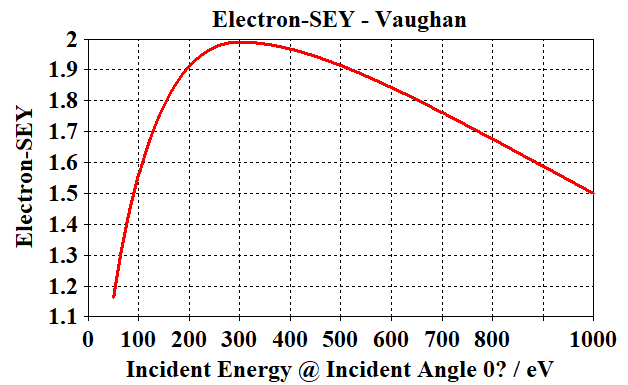
\includegraphics[width=0.4\textwidth]{pic/chapter3/铜的SEY.png} & 
        \hspace{5pt}
        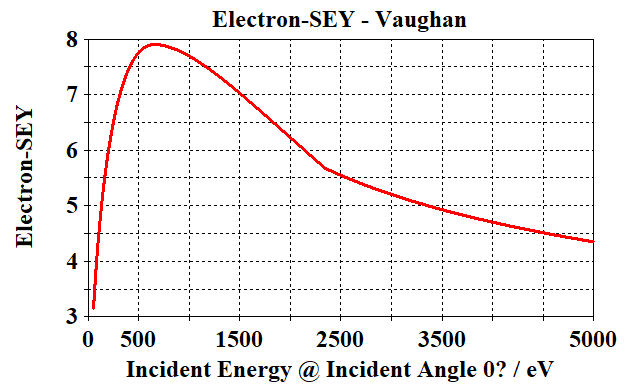
\includegraphics[width=0.4\textwidth]{pic/chapter3/蓝宝石的SEY.png}     \\
        \mbox{\small (a)铜二次电子发射曲线}                                                                               & 
        \mbox{\small (b)蓝宝石二次电子发射曲线}                                                                                  \\
    \end{tabular}
    \caption{Vaughan模型下材料的二次电子发射特性}
    \label{fig:X波段材料二次电子发射特性}
\end{figure}

为了方便进行二次电子发射曲线的设置,需要将窗片使用无氧铜外壳进行包覆。为了验证背景材料更改为无氧铜之后是否会对窗片本身的电磁特性产生影响,现在将背景材料更改为无氧铜进行关于S曲线的仿真。此时无氧铜的电导率被设置为$\sigma = 5.8 \times 10^7 S/m$。仿真结果在图\ref{fig:X无氧铜背景}中被展示,结果表明背景材料被更改为无氧铜并没有对S曲线产生太大的影响,可以使用无氧铜作为原先窗片的外壳进而进行后续的仿真。
\begin{figure}[!htb]
    \centering
    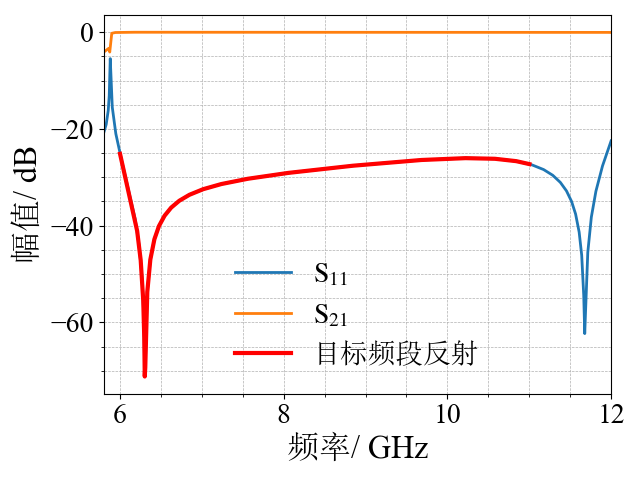
\includegraphics[width=0.5\linewidth]{pic/chapter3/X脊波导窗无氧铜.png}
    \caption{X波段脊波导无氧铜背景下的S曲线}
    \label{fig:X无氧铜背景}
\end{figure}

\subsubsection{使用Spark3D进行功率容量的计算}
为了方便后续的二次电子仿真,有必要使用CST中专门进行电子倍增仿真的Spark3D模块进行预先仿真。Spark3D模块不仅可以看出原先器件中哪些地方的电场强度更强,也可以根据已经设定好的二次电子发射曲线,来进行初步的功率容量仿真。这些预先的结果都为了进一步的使用CST进行PIC的仿真提供了方便,有助于减少进一步仿真中关于功率的迭代次数。首先将CST中频域求解器已经仿真好的电场磁场强度结果导出成Spark3D模块可以使用的$.f3e$格式,并且导入Spark3D,材料相关的二次电子发射曲线参考之前所找到的材料和\ref{fig:X波段材料二次电子发射特性},尽量做到跟PIC求解器中的二次电子发射曲线参数一致。Spark3D中的初始轰击电子的位置是随机的,其在每次仿真过程中并无法得到完全相同的功率容量。为了确保仿真结果的真实性,需要适当的增加Spark3D中的初始电子数目需要增加,本次在Spark3D中放置初始电子数目为800。

图片\ref{fig:X波段Spark3D中的电场}展示了脊波导窗中电场分布,参考文献\cite{guobao_2019_intera}中关于电场强度的说法,此时可以得知电场场强最强的部分是脊波导的脊,以及脊波导和窗中间的过渡部分的圆角矩形部分。由于器件工作在低频点时更容易被击穿,故此时在Spark3D中的激励信号被设置为6GHz的连续波。
\begin{figure}[!htb]
    \centering
    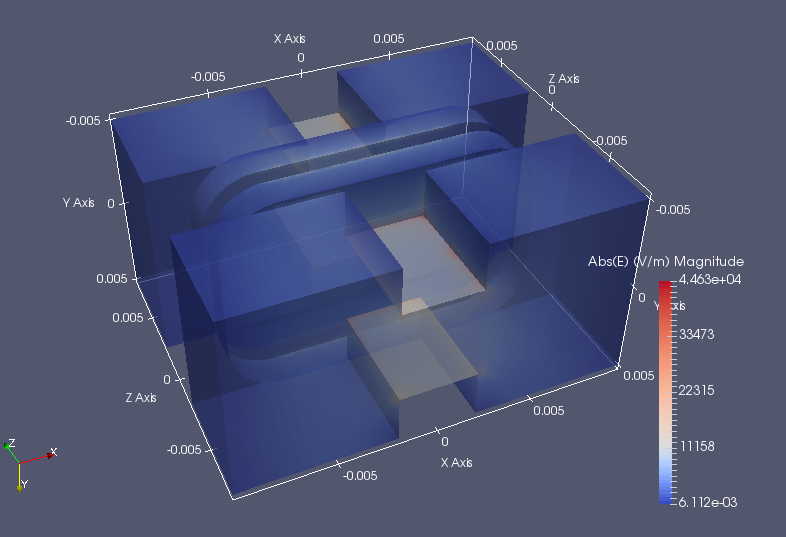
\includegraphics[width=0.5\linewidth]{pic/chapter3/X波段Spark3D中的电场.png}
    \caption{X波段脊波导Spark3D中的电场}
    \label{fig:X波段Spark3D中的电场}
\end{figure}

在仿真开始的时候Spark3D模块会在器件中放入一定树木的种子电子(图中放置的种子电子数目为8千个)并且使用设定频率的连续波进行激励。当一定时间后,初始被放置在器件中的电子数目没有归零的话,就判定为器件被击穿。结合以上分析与初始设定,此时使用Spark3D初步仿真得到窗片的功率容量为10kW,具体的Spark3d的仿真结果如图\ref{fig:X波段Spark3D中的功率}所示。图中横轴为仿真时间,纵轴为电子总数目。
\begin{figure}[!htb]
    \centering
    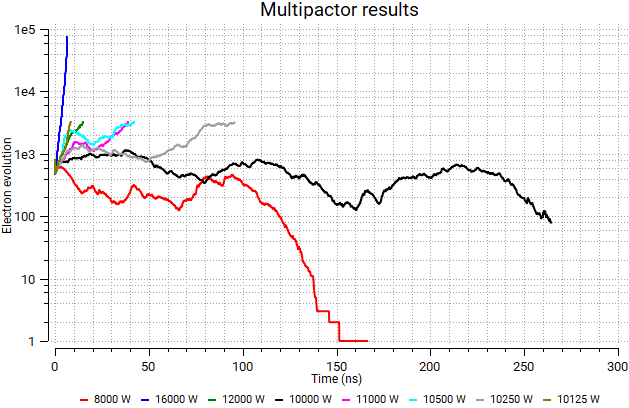
\includegraphics[width=0.5\linewidth]{pic/chapter3/X波段Spark3D中的功率.png}
    \caption{X波段脊波导Spark3D中计算的功率}
    \label{fig:X波段Spark3D中的功率}
\end{figure}

刚才的Spark3D仿真已经获取到了初始的窗片使用电子倍增方法计算的功率容量,接下来使用CST中的PIC求解器进行二次电子倍增相关功率容量的详细仿真。

\subsubsection{使用CST的PIC模块进行功率容量的计算}
不同于SPARK3D的材料设定,CST的PIC求解器不能设置背景材料的二次电子发射系数,此时需要对窗片套上一定厚度的外壳后进行进一步的二次电子仿真。为了方便建模,将原先的真空仿真模型外侧套上了一个宽和高比模型最外侧还要大2mm的立方体外壳,套上外壳之后的窗整体如图\ref{fig:X无氧铜外壳}所示。
\begin{figure}[!htb]
    \centering
    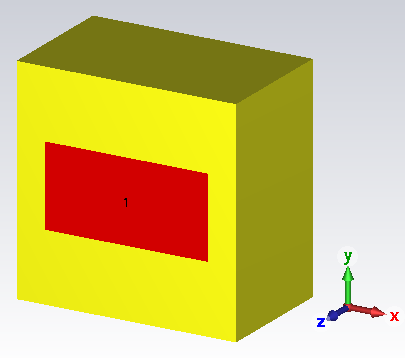
\includegraphics[width=0.4\linewidth]{pic/chapter3/X脊波导窗无氧铜外壳.png}
    \caption{X脊波导窗加上无氧铜外壳}
    \label{fig:X无氧铜外壳}
\end{figure}

此时CST的默认激励端口的信号为脉冲激励,并不符合实际上使用时候的输入信号模型,应该改为连续波激励。本次仿真所使用的是连续正弦信号激励,由于在实际使用的过程中,在低频更容易被击穿,故本次连续波激励信号的频率被设定为原规定频域(6-10 GHz)的最低频点6 GHz处。此时的连续波激励信号的时域图如图\ref{fig:X波导窗连续波激励信号}所示,连续信号的激励的时长并不是6.4ns,图中横轴只是为了方便查看信号而进行的缩放。经过初步的CST PIC仿真与设置粒子轨迹监视器发现,在正常工作功率范围内的连续波信号的激励情况下初始电子的消失时间约为90ns。根据以前的实验经验,连续波的激励时间和总仿真时间应该不低于这个时间的两倍,故连续波的正常激励时间和总仿真时间被设定为200ns。
\begin{figure}[!htb]
    \centering
    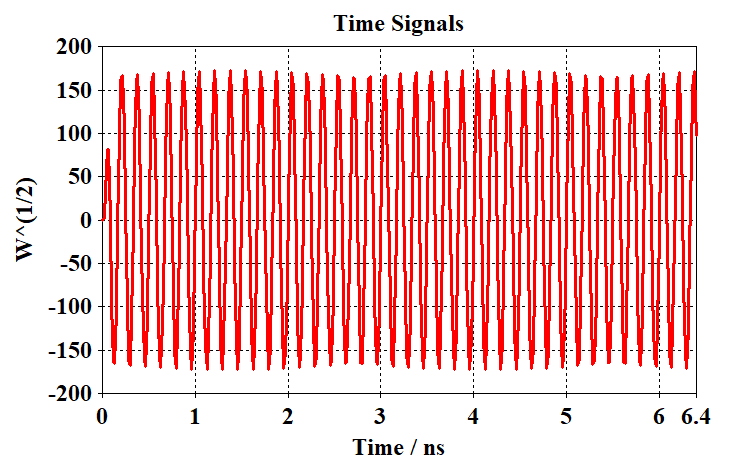
\includegraphics[width=0.5\linewidth]{pic/chapter3/X波段脊波导窗连续波激励信号.png}
    \caption{X波段脊波导窗连续波激励信号}
    \label{fig:X波导窗连续波激励信号}
\end{figure}

具体的仿真流程中,经常使用在器件中放置一定数目的电子作为初始的种子粒子,然后再使用电场来驱动这些粒子对器件的表面进行轰击,进而通过观察此时的初始粒子数目随着时间的的变化情况来判断器件是否被击穿。具体的放置种子粒子的密度以及判断器件的击穿标准在不同的文章中也不尽相同,但是可以选取几篇文章作为相应的参考。根据文章\cite{li_2021_novel_multipactor}中的描述,如果器件中的电子数目在信号驱动的情况下呈现出指数函数式的增长,那么就被视为期间会因为二次电子发射而击穿,如果器件中电子的数目随着信号的激励呈现出持续下降的趋势就被视为没有击穿。关于具体的种子粒子的放置,文献\cite{gonzalez_2015_experimental}在仿真同轴波导的时候,初始的种子粒子数目为500,判断其被击穿的条件为仿真过程中电子总数大于$10^4$;文献\cite{gonzalez_2016_multipactor}在仿真同轴波导时,初始的电子数目为$10^{12}$个,等效的电子密度为$4.83 \times 10^{17} m^{-3}$,由于激励信号并非使用正弦函数,故击穿的条件被设定为“20间隙击穿”法则;文献\cite{you_2015_highly}中在脊波导器件的最窄处填充了8000个电子,并且也是因为电子数目在正弦信号驱动情况下呈现指数增长才被视为击穿,如果是持续下降的电子趋势就被视为没有击穿。

综合上述文献的描述与仿真速度精度的要求,本文决定在填充初始电子时候选择电场强度最强的部分进行立方体形状的麦克斯韦能量分布的粒子源填充,而不是所有空白区域全部都进行初始能量相同的电子填充,并且填充的电子的密度不低于$10^9 m^{-1}$。如果器件中电子的数目随着信号的激励呈现出持续下降的趋势就被视为没有击穿;如果总粒子数目呈现出指数函数式的增长,那么在总粒子数目达到$5 \times 10^5$个之后便被视为击穿。结合之前在Spark3D中的预仿真,还有一种电子数量没有明显增长但是也没有明显减小的情况,此时其二次电子产生和电子的被吸收速率相近,在电子数目中达到了动态平衡,这种情况依然对器件有击穿的风险,故也被视为击穿。根据Spark3D和之前图\ref{fig:X频段脊波导窗低频点场强仿真}中的预先仿真,可以得知此时的电场场强最强的部分是脊波导的脊,以及脊波导和窗中间的过渡部分的圆角矩形部分,具体的填充区域示意图可见\ref{fig:X粒子填充区域}中所示。
\begin{figure}[!htb]
    \centering
    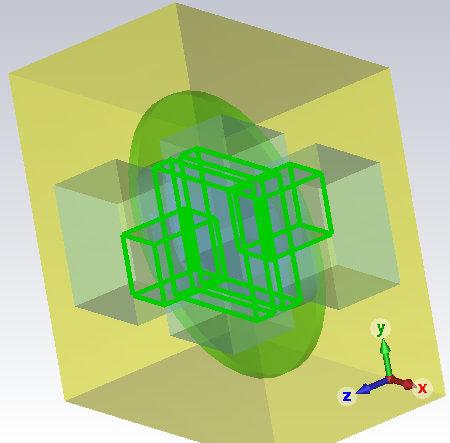
\includegraphics[width=0.25\linewidth]{pic/chapter3/粒子填充区域斜视图.png}
    \caption{X波段脊波导窗粒子填充区域}
    \label{fig:X粒子填充区域}
\end{figure}

在进行好了材料二次电子发射曲线、正弦连续波激励信号、初始麦克斯韦能量分布的电子的粒子填充和明确了因为电子倍增现象而击穿的规则之后,便可以对器件进行基于电子倍增现象的功率容量的仿真。仿真得到的整体粒子数目随着馈入连续波时间的变化而产生的变化的曲线被展示与图片\ref{fig:X波段脊波导窗基于电子倍增现象的功率容量仿真}中。从图片中可以看到,在馈入能量达到14.8kW之前,器件中粒子数目随着时间的变化呈现为持续下降的趋势;在能量到达15kW时电子数目达到动态平衡;但是在馈入连续波能量达到15.3kW之后,粒子数目呈现出持续增长趋势。根据上述分析便可以得出结论,X波段脊波导窗片在使用电子倍增理论进行仿真时,其功率容量为14.9kW。
\begin{figure}[!htb]
    \centering
    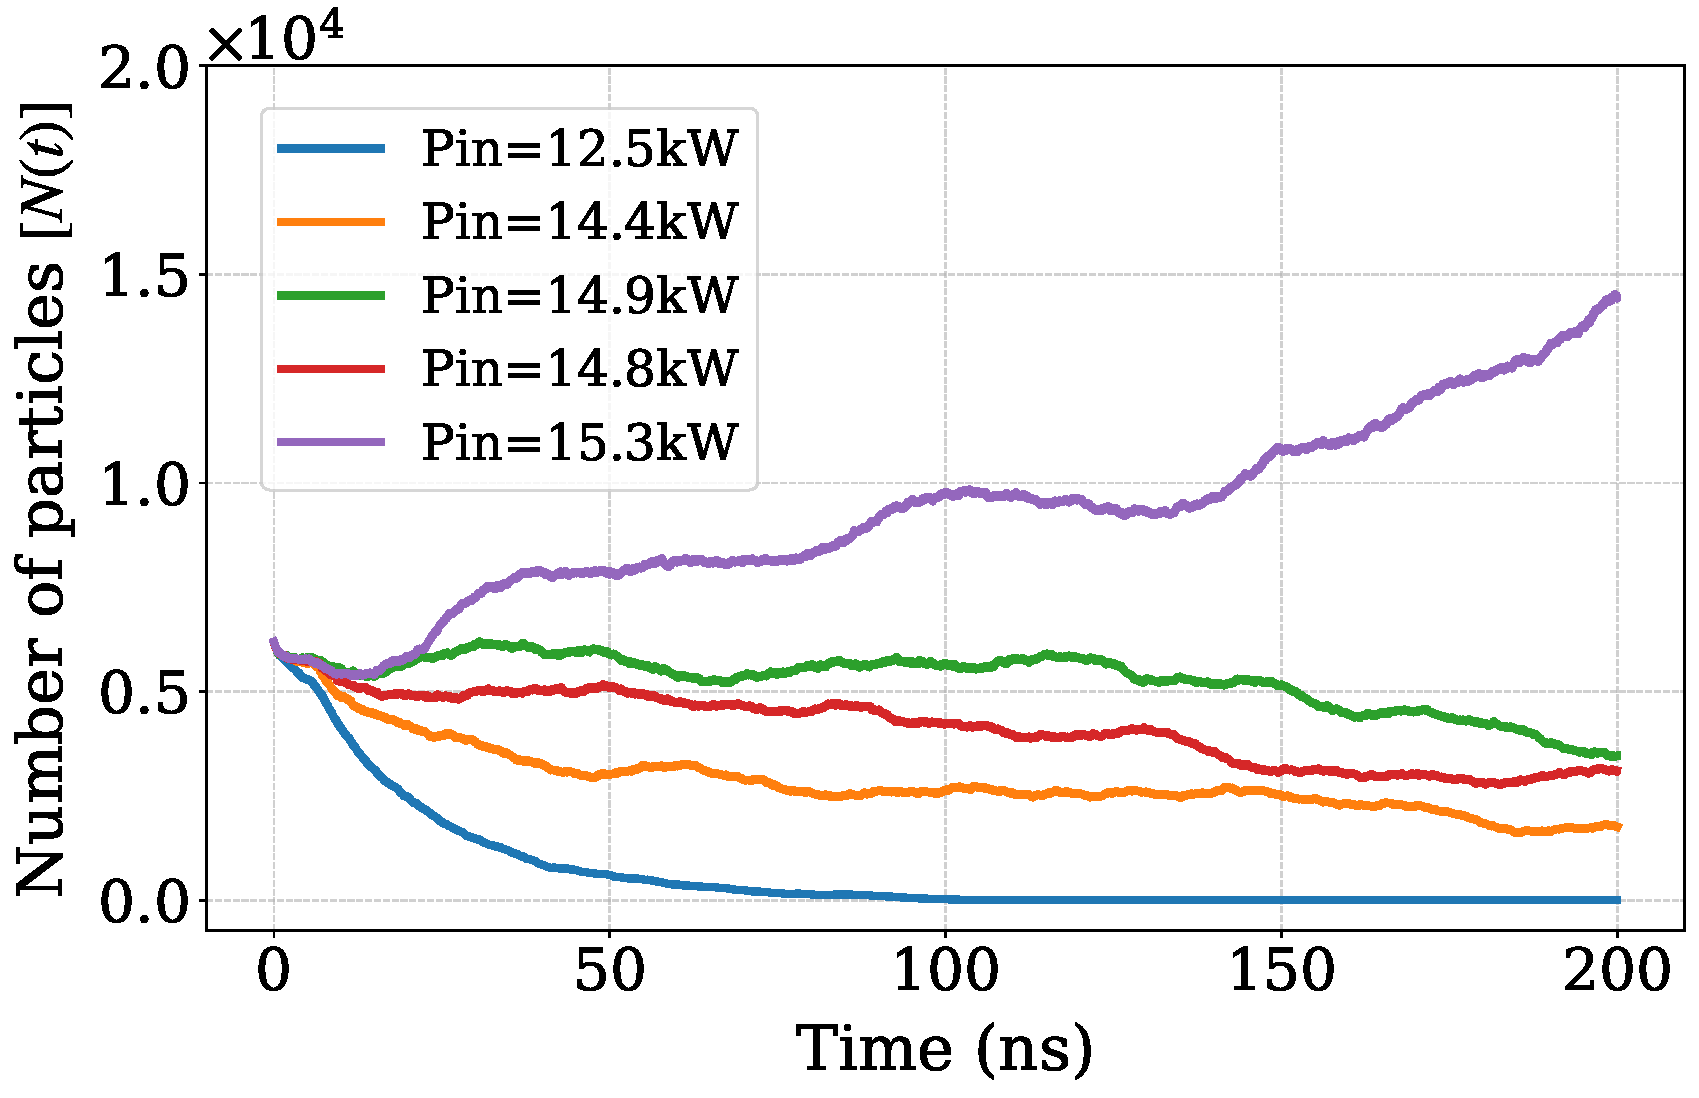
\includegraphics[width=0.5\linewidth]{pic/chapter3/particle_time_chapter3.pdf}
    \caption{X波段脊波导窗基于电子倍增现象的功率容量仿真}
    \label{fig:X波段脊波导窗基于电子倍增现象的功率容量仿真}
\end{figure}


\section{脊波导窗的多物理场分析}
在实际的窗片使用过程中,由于介质材料存在介质损耗,故窗片会产热。又由于窗片和金属波导的热膨胀系数\(\alpha\)不一致,故在窗片产热之后,二者的接触面会产生热应力。如果热应力过大的话,窗片可能会产生不可逆的损坏。其次,窗片上温度的分布在实际的使用过程中也是十分重要的,如果由于散热机构设计的问题导致窗片上温度的差值过大,可能会导致其内部热应力过大而损毁。故在进行实际的装配加工之前,对窗片的多物理场仿真分析是必不可少的。
\subsection{仿真环境的搭建}
本次仿真研究内容是使用有限元软件HFSS与ANSYS联合仿真,研究在一定的功率容量馈入时,窗片上应力与温度分布的情况。

ANSYS的热分析模块可以自由地添加热源,其中可以添加均匀体密度热源与面热源,但是这些热源都与窗片在实际工作过程中的产热不尽相符。根据之前的仿真分析,此时窗片的主要工作模式类似于过渡圆角矩形波导所对应的类似于\(TE_{01}\)的传输模式,这个模式在窗片的横截面上并不均匀,而场强越大的地方,单位体积内窗片介质产热的功率就越高。如果直接使用均匀分布的热源,会导致实际的产热与仿真出来的产热不一致。故本次使用HFSS与ANSYS之间的联合仿真,ANSYS将使用由HFSS模块所计算出来的窗片的体密度损耗作为窗片上介质损耗热源的依据,进而使用这些热源完成后续的温度以及应力的仿真。在ANSYS中,HFSS模块与其它模块的连接方式如图\ref{fig:ANSYSHFSS连接}所示。
\begin{figure}[!htb]
    \centering
    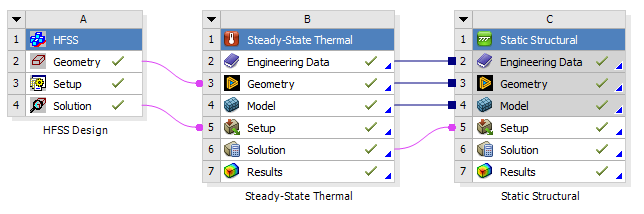
\includegraphics[width=0.5\linewidth]{pic/chapter3/HFSS-ANSYS模块组织.png}
    \caption{HFSS-Anasys联合仿真}
    \label{fig:ANSYSHFSS连接}
\end{figure}
HFSS模块计算窗片由于介质损耗而产生的体损耗,同时也分析铜制外壳由于金属损耗产生的表面金属损耗。在此之后,会将产生的损耗结果导入到后续的稳态热仿真模块中,稳态热仿真模块使用原先损耗结果产生的热并且求解出稳态热的温度场之后会将其导入到后续的稳态机械模块对其应力应变的结果进行分析。

为了方便对加工完成后的窗片的对流散热现象情况进行近似模拟,在原先的空气模型外侧加装了一个最薄处为2mm 的铜制的金属外壳。此时加装金属外壳后的窗片的外形与图\ref{fig:X无氧铜外壳}一致,但是此时为了拟合更加真实的焊接场景,将原先的整体铜制外壳进行了纵向分割。分别按照脊波导传输段、窗片与过渡波导段和脊波导传输段三个部分,分割后的整体视图如图\ref{fig:X频段铜制外壳分割后} (a)。并且如图\ref{fig:X频段铜制外壳分割后} (b)所示,HFSS的S仿真验证了此铜制外壳与分割不会对窗片的S参数产生影响。此时设置蓝宝石的损耗角正切被设定为\(\tan \delta = 0.0004\),铜的电导率被设定为\(\sigma = 5.8 \times 10^7 S/m\)。在完成建模之后,将模型导入HFSS模块进行关于损耗的仿真。此时馈入窗片的功率为5kW,为二次电子发射所计算的最大功率容量大约三分之一,馈入窗片的信号频率为8GHz。
\begin{figure}[!htb]
    \small
    \centering
    \begin{tabular}{@{\ }c@{\ }c}
        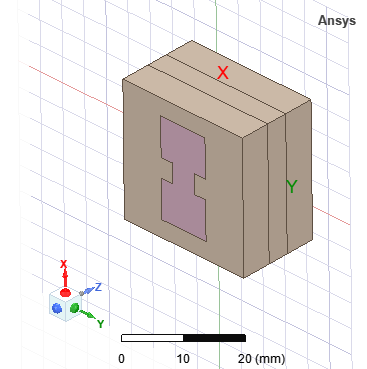
\includegraphics[width=0.3\textwidth]{pic/chapter3/铜制外壳分割后.png} & 
        \hspace{5pt}
        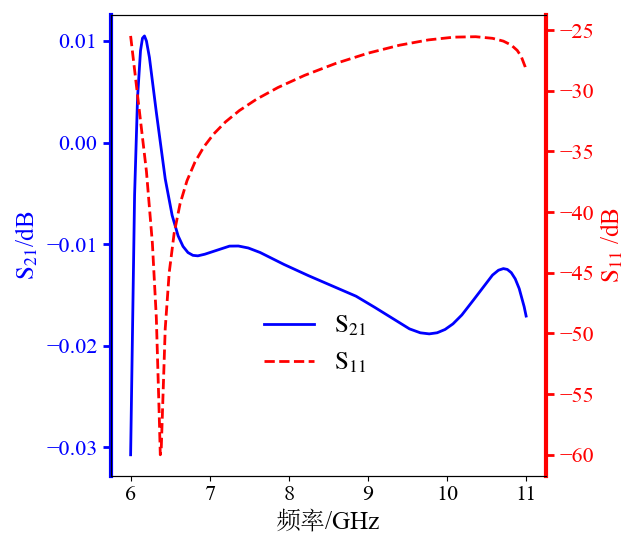
\includegraphics[width=0.3\textwidth]{pic/chapter3/分割后的S参数.png}     \\
        \mbox{\small (a)铜制外壳分割示意图}                                                                               & 
        \mbox{\small (b)分割后使用HFSS进行S参数的验证}                                                                                  \\
    \end{tabular}
    \caption{6-11GHz频段窗片铜制外壳分割与S参数验证}
    \label{fig:X频段铜制外壳分割后}
\end{figure}


\subsection{脊波导窗温度分布计算}
此时在HFSS中仿真得到的窗片的体积损耗分布如图\ref{fig:X频段窗损耗分布图} (a)所示,可以看到,此时因为窗片中损耗较高的地方对应了其中电场强度较大的部分,与预期相符。此时窗片中心部位对应的电场强度最高,故此时中心部位的介质体积损耗也最高,可以预计此时窗片中心部分的产热最多。通过HFSS的仿真,如图\ref{fig:X频段窗损耗分布图} (b)所示,可以看出来窗片的波导表面金属损耗主要集中于过渡圆角矩形波导与脊波导相接的波导壁处。结合之前的场强分析也可以看出来,此时金属损耗的最大值也正是最大场强所在的位置。经过HFSS的计算,此时窗片的介质损耗为2.96W,铜质金属外壳造成的金属表面损耗为5.09W。
\begin{figure}[!htb]
    \small
    \centering
    \begin{tabular}{@{\ }c@{\ }c}
        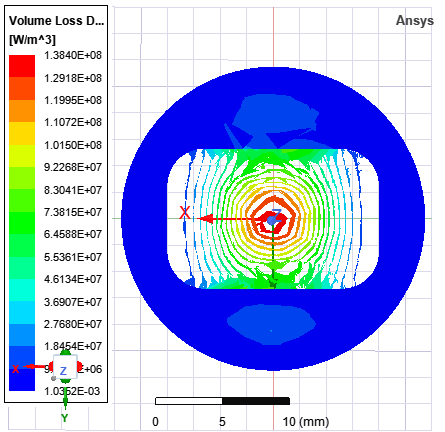
\includegraphics[width=0.3\textwidth]{pic/chapter3/X频段窗片体积损耗.png} & 
        \hspace{5pt}
        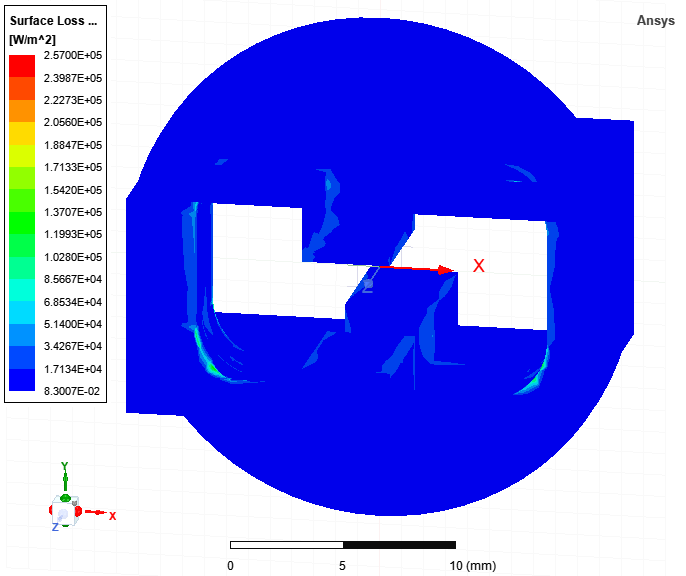
\includegraphics[width=0.3\textwidth]{pic/chapter3/X频段波导表面损耗.png}     \\
        \mbox{\small (a)窗片体积损耗}                                                                               & 
        \mbox{\small (b)窗片表面金属损耗}                                                                                  \\
    \end{tabular}
    \caption{6-11GHz频段窗片损耗分布}
    \label{fig:X频段窗损耗分布图}
\end{figure}

假设窗片外侧的铜制外壳在与空气进行强制对流散热,设置铜制外壳的空气对流的对流系数为\(300 W/ (m \cdot K)\),此时外界热对流的设置如图\ref{fig:X频段窗片对流辐射散热} (a)所示,室温被设置为20℃。关于对流散热面的设置窗片表面由于焊接在器件内部,此时假设其在纵向波导内部无热对流,只假设其暴露在真空的单元存在辐射散热,并且取辐射因子为0.22。此时窗片的辐射散热设置如图\ref{fig:X频段窗片对流辐射散热} (b)所示,本次计算并未选择一整个窗片表面进行辐射散热设置,而是选择了暴露在真空中的窗片部分进行辐射设置。此时窗片与金属波导之间的接触面可能存在缝隙或者气泡,并不能视作一体进行热传导,故需要为金属波导和窗片的接触面设置相应的热阻值。根据参考文献\cite{jiang_2022_design}中的描述,需要将接触面的热阻值设为8000\(W / (m^2 \cdot K)\)。但是金属之间的接触很紧密,故可以将其设置为一体来进行热传导分析。
\begin{figure}[!htb]
    \small
    \centering
    \begin{tabular}{@{\ }c@{\ }c}
        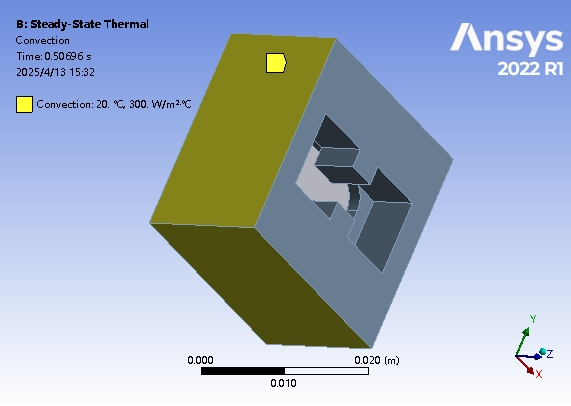
\includegraphics[width=0.3\textwidth]{pic/chapter3/窗片对流系数.png} & 
        \hspace{5pt}
        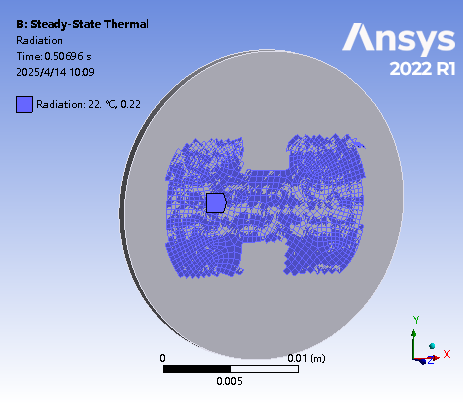
\includegraphics[width=0.3\textwidth]{pic/chapter3/辐射单元选择.png}     \\
        \mbox{\small (a)对流散热设置}                                                                               & 
        \mbox{\small (b)辐射散热设置}                                                                                  \\
    \end{tabular}
    \caption{6-11GHz频段窗片对流辐射散热}
    \label{fig:X频段窗片对流辐射散热}
\end{figure}

此时关于材料的热与膨胀系数的设置可以参考文章\cite{thumm_stateart_2020},此时设置蓝宝石的密度为\( \rho_{Sapphire}= 4 \times 10^3 kg/ m^3\),各向同性热膨胀系数为\(\alpha_{Sapphire} = 5.5 \times 10 ^{-6}K^{-1}\),此时杨氏模量为\( E_{Sapphire}= 385 GPa \),泊松比为\( \nu_{Sapphire}= 0.22 \),各向同性导热率为\(k_{Sapphire} =40 W/(m \cdot K)\)。此时蓝宝石材料的抗弯强度可以通过文章\cite{hanyong_diff_2011}中找出,此时抗弯系数为\(\sigma_{f} = 320MPa\)。蓝宝石的比热容\(c_p\)为\(0.8 J/ (g \cdot K)\)。为了方便后续的查阅与对比,将刚才找到的蓝宝石材料属性汇总为表格\ref{tab:AlOStateOfArt}。将这些材料的系数输入ANSYS之后便可以进行稳态热与稳态机械结构的仿真。使用公式\ref{eq:临界温差}可以得出此时蓝宝石的温差的极限值为\(\Delta T_{Sapphire} = 126.76 ^\circ C\)。

\begin{table}[!htb]
    \caption{蓝宝石材料属性}
    \label{tab:AlOStateOfArt}
    \resizebox{\columnwidth}{!}{%
    \begin{tabular}{ccccccccc}
    \toprule[1.5pt]

    % \hline
    材料       & \begin{tabular}[c]{@{}c@{}}比热容 $c_p$\\ $J / (g \cdot K)$\end{tabular} & \begin{tabular}[c]{@{}c@{}}导热率 k\\ $W/(m \cdot K)$\end{tabular} & \begin{tabular}[c]{@{}c@{}}热膨胀系数 $\alpha$\\ $\times 10 ^{-6} K^{-1}$\end{tabular} & \begin{tabular}[c]{@{}c@{}}密度 $\rho$\\ $kg/m^3$\end{tabular} & 泊松比 $\nu$ & \begin{tabular}[c]{@{}c@{}}杨氏模量 E\\ GPa\end{tabular} & \begin{tabular}[c]{@{}c@{}}抗弯系数 $\sigma$\\ MPa\end{tabular} & \begin{tabular}[c]{@{}c@{}}极限温差 $\Delta T$\\ ℃\end{tabular} \\ \hline
    蓝宝石 & 0.8                                                                  & 40                                                             & 5.5                                                                               & 4000                                                         & 0.22       & 385                                                  & 320                                                         & 126.76                                                          \\ %\hline
    \bottomrule[1.5pt]
    \end{tabular}%
    }
\end{table}

首先对窗片进行温度场分析,根据图\ref{fig:X输入温度场} (a)显示,此时窗片的温度主要集中于窗片的中心部分,与窗片所传输的电场场强分布相符。并且此时窗片上最高温度为47.02℃,最低温度为35.65℃,温差为11.37℃,小于之前所计算出来的温差的极限值。故窗片已经通过了温度差检验,不会因为温差而导致的热应力所损坏。ANSYS显示此时的窗片的平均温度为38.14℃,满足使用需求。
通过观察可以看到,此时窗片的温度分布并不是与角向无关的,温度沿y轴方向和x轴方向的变化曲线可以详见于图\ref{fig:X输入温度场} (b)中。虽说两条曲线的起点和终点的位置相同,但是此时温度沿y方向下降的速度要相比于沿x方向下降的速度要快得多。在实际的应用过程中应该注意窗片y轴方向上的温度差,以免此方向因为温差过大导致窗片碎裂。
\begin{figure}[!htb]
    \small
    \centering
    \begin{tabular}{@{\ }c@{\ }c}
        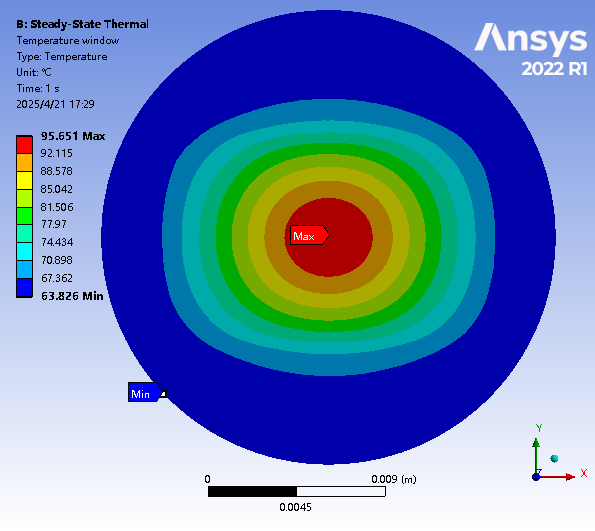
\includegraphics[width=0.3\textwidth]{pic/chapter3/X频段温度分布.png} & 
        \hspace{5pt}
        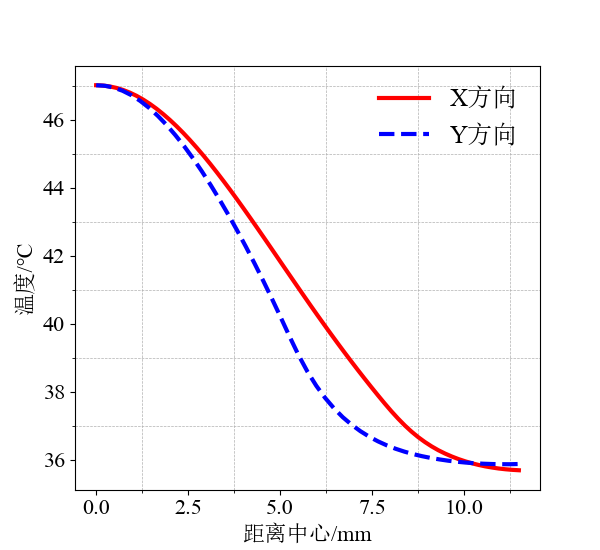
\includegraphics[width=0.3\textwidth]{pic/chapter3/窗片温度沿半径分布.png}     \\
        \mbox{\small (a) 温度分布云图}                                                                               & 
        \mbox{\small (b) 温度沿x方向和y方向的变化曲线}                                                                                  \\
    \end{tabular}
    \caption{窗片温度分布}
    \label{fig:X输入温度场}
\end{figure}

\subsection{脊波导窗的热应力分析}
ANSYS中可以直接查看到窗片的应力大小,为了方便分析窗片被安装在波导上之后的热应力大小,设置波导纵向的两侧端口为固定端面。为了使得应力分析更符合真实情况,此时窗片与中间铜制外壳之间的接触面被设定为Rough接触条件,此接触条件禁止接触面切向滑动但是允许其发生法向分离。铜制外壳切片之间的接触面的边界条件设定为Bonded,即完全不会因为形变发生任何位移或者滑动。此时边界条件的设置可以详见图\ref{fig:X频段接触面边界条件}所示。
\begin{figure}[!htb]
    \small
    \centering
    \begin{tabular}{@{\ }c@{\ }c}
        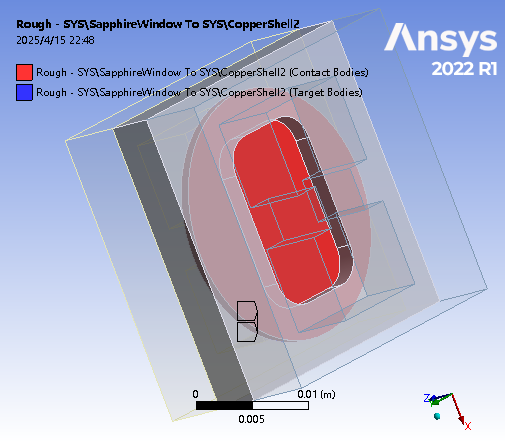
\includegraphics[width=0.3\textwidth]{pic/chapter3/金属外壳2与窗片间的接触条件.png} & 
        \hspace{5pt}
        \includegraphics[width=0.3\textwidth]{pic/chapter3/金属外壳3与2之间的接触条件.png}     \\
        \mbox{\small (a) Rough 接触条件}                                                                               & 
        \mbox{\small (b) 金属外壳间的Bounded接触条件}                                                                                  \\
    \end{tabular}
    \caption{6-11GHz频段窗片接触面边界条件}
    \label{fig:X频段接触面边界条件}
\end{figure}

由于蓝宝石在受热膨胀之后会与外侧的铜制外壳发生挤压,如果挤压的应力过大便会造成窗片损毁,此时使用后续稳态机械求解器所计算的与外侧铜壳之间发生的挤压进而带来的机械应力如图\ref{fig:X输入应力分布}所示。此时正面的应力分布如图\ref{fig:X输入应力分布} (a)所示;此时侧面的应力分布如图\ref{fig:X输入应力分布} (b)。综合来看,主要应力位于正面和外侧铜壳之间的接触面。
\begin{figure}[!htb]
    \small
    \centering
    \begin{tabular}{@{\ }c@{\ }c}
        \includegraphics[width=0.4\textwidth]{pic/chapter3/窗片正面应力分布.png} & 
        \hspace{5pt}
        \includegraphics[width=0.4\textwidth]{pic/chapter3/窗片侧面应力分布.png}     \\
        \mbox{\small (a) 窗片正面应力分布}                                                                               & 
        \mbox{\small (b) 窗片侧面应力分布}                                                                                  \\
    \end{tabular}
    \caption{6-11GHz输入窗应力分布云图}
    \label{fig:X输入应力分布}
\end{figure}

此时应力主要出现在圆形窗与圆角矩形过渡段的接触边界处,以及窗片圆边沿处。此时窗片上最大应力大小为84.06MPa,最小为13.61MPa,热应力小于材料的抗弯强度\(\sigma_f = 320\)MPa,其不会因为最大热应力而导致损毁。经过热应力的分析可以得出相关结论,此时窗片在实际的加工使用时应该注意其与圆角矩形过渡段之间的接触边沿处的应力防护,因为这些边沿处最容易产生因为应力过大而造成的损坏。

因为蓝宝石的抗压缩能力较强但是并不抗拉伸,此时除了分析窗片的总体应力之外还应该注意窗片的不同方向的应力分布情况,针对窗片不同方向应力的分布如图\ref{fig:X输入不同方向应力分布} 中所示。图\ref{fig:X输入不同方向应力分布} (c)展示了窗片的径向应力,此时中心部分和与圆角矩形的长边楞接触的部分的应力主要为挤压应力,但是此时最大值为33.67MPa小于蓝宝石的抗弯强度\(\sigma_f=320\)MPa,并不会因为挤压而损毁。
值得注意的是此时窗片的上下沿部分出现了拉伸应力,最大到达了35.3MPa,但是根据文献\cite{schmid1998effects}显示,此时拉伸应力远小于蓝宝石的拉伸极限300MPa,故窗片依然处于安全情况之下。具体焊接时也应注意避免让窗片上下边沿与铜制外壳的接触部分产生过大应力,避免窗片因为拉伸应力而导致损毁。

此时观察图\ref{fig:X输入不同方向应力分布} (a)和(b)可以发现,窗片的角向应力最大可以达到35.46MPa,主要出现位置为窗片与铜制外壳相接触的上下边沿位置;z轴方向的应力最大可以到达80.01MPa,主要出现位置为窗片与圆角矩形过渡波导接触处。说明两侧的焊接好的铜制外壳也会对窗片产生角向与纵向的挤压,但是此时挤压的应力大小小于窗片材料的抗弯强度,暂无法对窗片产生损毁。
\begin{figure}[!htb]
    \small
    \centering
    \begin{tabular}{@{\ }c@{\ }c}
        \includegraphics[width=0.29\textwidth]{pic/chapter3/Xy轴角向应力.png} & 
        \hspace{5pt}
        \includegraphics[width=0.29\textwidth]{pic/chapter3/Xz轴纵向应力.png}     \\
        \mbox{\small (a) y轴角向应力}                                                                               & 
        \mbox{\small (b) z轴纵向应力}                                                           \\[6bp]
        \multicolumn{2}{c}{\includegraphics[width=0.29\textwidth]{pic/chapter3/Xx轴径向应力.png}} \\  % 使用跨列居中
        \multicolumn{2}{c}{\mbox{\small (c) x轴径向应力}}             
    \end{tabular}
    \caption{6-11GHz脊波导圆窗不同方向应力云图}
    \label{fig:X输入不同方向应力分布}
\end{figure}

\subsection{脊波导窗的热形变分析}
在窗片和外壳发生受热形变之后,有可能会导致整体结构参数出现变化,进而导致窗片的工作性能低于原先的设计值。有必要针对原结构进行热形变相关的分析。

首先是整体结构的形变分析,整体结构的形变详见于图\ref{fig:X整体结构形变}中。此时整体结构形变主要发生在金属外壳与窗片焊接的一节,最大形变量为0.004mm。脊波导处的形变量最大值为0.002mm,出现在脊波导突出的脊处,过渡圆角矩形波导的最大型变量为0.002mm。结合之前小节中的\ref{subsec:脊波导窗的参数敏感度分析}中的参数敏感度分析,此形变量较为微小,无法对结构造成能够改变S传输特性的明显变化。
\begin{figure}[!htb]
    \centering
    \includegraphics[width=0.5\linewidth]{pic/chapter3/X输入窗与波导.png}
    \caption{6-11GHz脊波导圆窗整体结构形变云图}
    \label{fig:X整体结构形变}
\end{figure}

由于之前参数敏感度分析部分得出结论,窗片的半径和厚度对窗片整体的S参数有较为明显的影响,有必要对窗片的形变进行详细的分析。

窗片的整体形变量详见于\ref{fig:X输入窗形变} (a)中,发现窗片最大形变量为0.002mm。此时窗片发生主要整体形变的位置为外侧边沿与铜制外壳的接触点处,并且主要是x轴侧与铜制外壳的接触点。

此时窗片径向形变详见于\ref{fig:X输入窗形变} (b)中,其表示了窗片在受热膨胀时其沿着半径发生膨胀或者收缩的量。此时窗片的径向形变量的最大值为0.002mm,主要发生位置和总形变量类似,位于x轴边沿处和铜制外壳相接处的地方形变量最大。可以看到,此时径向形变的大小和整体形变的大小相当,说明径向形变为最主要的形变类型。并且此时径向形变主要为向外伸展的形变,说明了窗片在受热之后有着径向膨胀的倾向。

沿着z轴的形变如图\ref{fig:X输入窗形变} (c)所示,此时窗片的形变表明了其在经过热膨胀后厚度变化的量。此时窗片沿着z轴形变量的最大值为\(6 \times 10^{-5}\)mm,主要发生形变的位置为窗片的中心。但是此时z轴厚度变化极为微小,并不足以对窗片的厚度产生明显影响。

综上所述,此时窗片的半径形变和厚度形变的程度都不足以影响窗片的整体S参数。通过对6-11GHz输入窗的多物理场仿真,可以得知此时的窗片设计符合5kW的功率输入要求。
\begin{figure}[!htb]
    \small
    \centering
    \begin{tabular}{@{\ }c@{\ }c}
        \includegraphics[width=0.29\textwidth]{pic/chapter3/X输入窗总形变.png} & 
        \hspace{5pt}
        \includegraphics[width=0.29\textwidth]{pic/chapter3/X输入窗径向形变.png}     \\
        \mbox{\small (a) 总体形变}                                                                               & 
        \mbox{\small (b) 径向形变}                                                           \\[6bp]
        \multicolumn{2}{c}{\includegraphics[width=0.29\textwidth]{pic/chapter3/X输入窗厚度形变.png}} \\  % 使用跨列居中
        \multicolumn{2}{c}{\mbox{\small (c) 厚度形变}}             
    \end{tabular}
    \caption{6-11GHz脊波导圆窗形变云图}
    \label{fig:X输入窗形变}
\end{figure}

\subsection{14kW输入时的窗片损坏风险}
为了分析使用二次电子发射时的最大功率容量时窗片的损坏风险,此时将窗片的输入功率从5kW增加到14kW。使用HFSS-ANSYS联合仿真得到窗片的应力结果如图\ref{fig:X14kW时候的应力云图}所示。

此时窗片的应力分布和之前的5kW输入时的应力分布类似,但是绝对数值发生了变化。此时窗片正面应力的最大值为279.68MPa,已经可以与蓝宝石的抗弯强度\(\sigma_f = 320\)MPa相比,如果在焊接过程中引入一定的应力,窗片的内部应力极容易大于抗弯强度进而导致窗片的损毁。

其次窗片的不同方向的应力所占比与原先的类似,但是此时z轴方向的挤压应力占主要比例。此时z轴方向的应力最大值为267.49MPa,出现在铜壳的圆角矩形过渡段的长边中点与窗片所接触处再稍微往上处。此时z轴纵向应力也极为接近蓝宝石的抗弯强度。这表示,此结构的圆形窗片在14kW的馈入功率中,可能会因为圆角矩形过渡段与窗片接触处的纵向的应力而导致损毁。

这部分仿真也进一步说明了在实际窗片设计过程中,使用多物理场验证功率容量结果的必要性。
如果直接使用前面小节\ref{subsec:X二次电子倍增功率容量}中的二次电子发射法或者小节\ref{subsec:X最大场强功率容量}的最大场强法作为实际窗片的功率容量。那么很容易导致窗片在实际的应用过程中因为应力过大而损坏。
\begin{figure}[!htb]
    \small
    \centering
    \begin{tabular}{@{\ }c@{\ }c}
        \includegraphics[width=0.29\textwidth]{pic/chapter3/14k窗片正面应力分布.png} & 
        \hspace{5pt}
        \includegraphics[width=0.29\textwidth]{pic/chapter3/14kXx轴径向应力.png}     \\
        \mbox{\small (a) 窗片正面应力分布}                                                                               & 
        \mbox{\small (b) x轴径向应力}                                                           \\[6bp]
        \includegraphics[width=0.29\textwidth]{pic/chapter3/14kXy角向应力.png} & 
        \hspace{5pt}
        \includegraphics[width=0.29\textwidth]{pic/chapter3/14kXz轴径向应力.png}     \\
        \mbox{\small (a) y轴角向应力}                                                                               & 
        \mbox{\small (b) z轴纵向应力}             
    \end{tabular}
    \caption{6-11GHz脊波导圆窗14kW时应力云图}
    \label{fig:X14kW时候的应力云图}
\end{figure}

\section{脊波导窗模式变换结构设计}
\subsection{模式变换结构类型选择}
根据之前\ref{fig:6-11GHzDRW}的脊波导几何参数可以看出,此时的脊波导并非公用的标准脊波导,没有标准的同轴转脊波导的模式转换器。如果想要进行进一步的脊波导窗的测试,有必要设计脊波导转同轴的模式转换器。此时结合实际的测试情况,由于之前已经有标准矩形波导转同轴的模式转换器,并且在需要带宽内满足反射系数$S_{11}$<-25dB的反射系数要求。故设计脊波导到标准矩形波导的模式转换器。根据查表显示,标准矩形波导WR112的参数为28.499*12.624mm,本波导的截止频率为5.25GHz,低于所需要频段的最低频点。并且为了标准矩形波导到脊波导之间测试件的纵向长度足够短足够紧凑,本文选取的模式变换主要结构为阶梯过渡,而不是渐变过渡。

经过上述分析,再加上CST方面的优化,得到了如图\ref{fig:脊波导模式变换} (a)所示的模式变换结构:

\begin{figure}[!htb]
    \small
    \centering
    \begin{tabular}{@{\ }c@{\ }c}
        \includegraphics[width=0.45\textwidth]{pic/chapter3/脊波导模式变换.png} & 
        \hspace{5pt}
        \includegraphics[width=0.35\textwidth]{pic/chapter3/模式变换纵向长度.png}     \\
        \mbox{\small (a) 脊波导模式变换总体视图}                                                                               & 
        \mbox{\small (b) 模式变换纵向视图}                                                                                  \\
    \end{tabular}
    \caption{脊波导模式变换}
    \label{fig:脊波导模式变换}
\end{figure}

靠近z轴正轴的脊波导为之前\ref{fig:6-11GHzDRW}中所示的双脊波导,而原理z轴正轴的矩形波导即为之前所提到的WR112标准矩形波导。关于阶梯过度过渡段的各个段落的纵向长度如图片\ref{fig:脊波导模式变换} (b)所示,图中所示的两端阶梯过渡段长度均相等,过渡段的总体长度为21.22mm。

此时过渡段中间两个脊波导的脊的宽度与之前所设计的脊波导的脊宽相同,但是脊的高度和脊波导外侧的尺寸不同,进而能够形成阶梯状过渡。过渡段脊波导的详细几何参数如图\ref{fig:过渡段几何参数}所示,其中\ref{fig:过渡段几何参数} (a)展示了过渡段中靠近窗片的脊波导几何参数,\ref{fig:过渡段几何参数} (b)展示了过渡段中靠近标准矩形波导的脊波导几何参数。

\begin{figure}[!htb]
    \small
    \centering
    \begin{tabular}{@{\ }c@{\ }c}
        \includegraphics[width=0.45\textwidth]{pic/chapter3/靠近窗片的脊波导过渡段.png} & 
        \hspace{5pt}
        \includegraphics[width=0.45\textwidth]{pic/chapter3/靠近标准矩形波导的脊波导过渡段.png}     \\
        \mbox{\small (a)靠近窗片的脊波导过渡段几何参数}                                                                               & 
        \mbox{\small (b)靠近标准矩形波导的脊波导过渡段几何参数}                                                                                  \\
    \end{tabular}
    \caption{过渡段几何参数}
    \label{fig:过渡段几何参数}
\end{figure}

\subsection{模式变换结构的S参数仿真}
此时过渡段的几何参数已经确定,在将过渡段整体耦合到窗片之前应该单独对过渡段进行S参数仿真。由于1端口(此时为脊波导端口)与2端口(此时为标准矩形波导端口)并不完全一致,故需要分别分析过渡段结构在1端口馈入和2端口馈入时候的情况。仿真结果如图\ref{fig:过渡段不同端馈入的S参数}中所示,其中\ref{fig:过渡段不同端馈入的S参数} (a)展示了脊波导馈入能量时候的S参数,\ref{fig:过渡段不同端馈入的S参数} (b)展示了标准矩形波导馈入能量时候的S参数,此时在两种情况下反射系数$S_{11}$均在频段6-11GHz之内小于-20dB:

\begin{figure}[!htb]
    \small
    \centering
    \begin{tabular}{@{\ }c@{\ }c}
        \includegraphics[width=0.35\textwidth]{pic/chapter3/一端口馈入.png} & 
        \hspace{5pt}
        \includegraphics[width=0.35\textwidth]{pic/chapter3/二端口馈入.png}     \\
        \mbox{\small (a)脊波导馈入能量}                                                                               & 
        \mbox{\small (b)标准矩形波导馈入能量}                                                                                  \\
    \end{tabular}
    \caption{过渡段不同端S参数}
    \label{fig:过渡段不同端馈入的S参数}
\end{figure}

此时将过渡段的对应端口连接到脊波导窗两端,整体的结构如图\ref{fig:脊波导窗的整体测试结构与S参数} (a)所示,此时窗片两端均使用阶梯过渡过渡到标准矩形波导WR112。

\begin{figure}[!htb]
    \small
    \centering
    \begin{tabular}{@{\ }c@{\ }c}
        \includegraphics[width=0.35\textwidth]{pic/chapter3/脊波导窗整体测试结构.png} & 
        \hspace{5pt}
        \includegraphics[width=0.35\textwidth]{pic/chapter3/脊波导窗整体S参数.png}     \\
        \mbox{\small (a)脊波导窗的整体测试结构}                                                                               & 
        \mbox{\small (b)脊波导窗整体测试结构S参数}                                                                                  \\
    \end{tabular}
    \caption{脊波导窗的整体测试结构与S参数}
    \label{fig:脊波导窗的整体测试结构与S参数}
\end{figure}

此时针对整体接上过渡段之后的窗片进行S参数仿真,得到的结果如图\ref{fig:脊波导窗的整体测试结构与S参数} (b)所示,此时在频带范围之内(6-11GHz),整体的反射系数也均小于-20dB,满足测试的需求。


\section{本章小结}
本小节首先针对需求设计了一款能够用于6-11GHz的脊波导圆窗,窗片材质选取为蓝宝石,设计完成后满足在频段6-11GHz内反射系数\(S_{11}\)<-20dB的需求。并且之后针对脊波导窗进行了关于参数敏感度相关的分析,分析结果表示,此时过渡段的厚度trh的影响较大,最大可扰动范围为0.47mm。
在此之后,针对脊波导窗片的功率容量进行了相应的计算,在计算的途中,分别使用了最大场强法、基于二次电子倍增的分析方法。其中最大场强法分析时,如果此时击穿场强为30kV/cm,那么其功率容量为3.1kW;使用二次电子倍增法所计算的窗的功率容量为14.8kW。
之后,本文对窗的多物理场方面进行了相应的分析,此时窗片的输入功率为5kW,窗片在外壳铜使用空气强对流降温的情况下,其温差为11.37℃,远小于窗片材料的温差极限值126.76℃。
并且此时窗片的热应力最大值为84.06MPa小于蓝宝石材料的抗弯强度\(\sigma_f = 320\)MPa,其不会因为热应力而导致损毁。分析不同方向的应力大小时发现,宝石窗的径向拉伸应力为35MPa,小于材料的拉伸极限300MPa。窗片的z轴纵向应力与y轴角向应力均低于材料的抗弯强度。故此时窗片也不会因为应力过大而损毁。
并且因为热导致的形变大小较小,结合参数的敏感度分析发现热形变不会导致窗片的工作参数产生较大的变化。
之后为了方便窗片进行进一步的加工测试,设计了窗片与标准波导WR112之间的阶梯过渡段并进行了仿真。仿真结果显示整体结构在6-11GHz内反射系数低于-20dB,满足测试需求。

\chapter{L 波段宽频带脊波导窗的设计}
\section{引言}
此时仿照之前的6-11GHz 脊波导输入窗进行L 波段宽频带脊波导窗的设计,此时由于需要与前面的L 波段脊波导器件进行直接连接,故L 波段脊波导参数已经被确定,无需对L 波段脊波导进行相应的几何参数设计。关于L 波段脊波导参数,可以见图\ref{fig:L波段脊波导结构} (a)中;图片\ref{fig:L波段脊波导结构} (b)展示了脊波导标红的四条边,为了防止脊波导在实际使用过程中电场幅值过大,便将此标红的四条边进行半径为0.5mm的倒圆角的处理。

\begin{figure}[!htb]
    \small
    \centering
    \begin{tabular}{@{\ }c@{\ }c}
        \includegraphics[width=0.4\textwidth]{pic/chapter4/L波段脊波导几何参数.png} & 
        \hspace{5pt}
        \includegraphics[width=0.4\textwidth]{pic/chapter4/脊波导倒圆角边.png}     \\
        \mbox{\small (a)L波段脊波导几何参数}                                                                               & 
        \mbox{\small (b)脊波导倒圆角的边}                                                                                  \\
    \end{tabular}
    \caption{L波段脊波导结构}
    \label{fig:L波段脊波导结构}
\end{figure}

其中L 波段的脊波导的具体的参数为$a=63mm, b=32mm, s=29mm, d=5mm$此时脊波导为了减少减小最大场强,增大功率容量,防止击穿的考量,在脊波导的两个脊部位进行了倒圆角的设计,倒圆角的尺寸为0.5mm。此时L 波段所需的设计频段为1.14-1.6GHz,此时将脊波导几何参数带入判别式\ref{eq:DRW_constraints}的中进行检验,可以发现此时的$s / a$ =0.46>0.45不满足应用公式的约束条件。但是将\ref{eq:DRW_closed}的算式带入,对L 波段脊波导的截止频率进行计算,可以得到$f_c$=1.073GHz,计算结果与如图\ref{fig:L波段脊波导初步仿真} (a)中的CST中仿真的截止频率1.072GHz相接近。此时仿真脊波导在需要频带(1.13-1.4GHz )内的反射系数可以得到如图\ref{fig:L波段脊波导初步仿真} (b)的结果,此时可以看到,在1.13-1.4GHz 的所需频段之内,此时的反射系数$S_{11}<-25dB$,满足匹配要求,可以作为设计窗片所需的脊波导。

\begin{figure}[!htb]
    \small
    \centering
    \begin{tabular}{@{\ }c@{\ }c}
        \includegraphics[width=0.45\textwidth]{pic/chapter4/脊波导截止频率仿真.png} & 
        \hspace{5pt}
        \includegraphics[width=0.45\textwidth]{pic/chapter4/L波段脊波导S参数.png}     \\
        \mbox{\small (a)L频段截止频率仿真}                                                                               & 
        \mbox{\small (b)L频段脊波导S参数}                                                                                  \\
    \end{tabular}
    \caption{L波段脊波导初步仿真}
    \label{fig:L波段脊波导初步仿真}
\end{figure}



此时仿照之前的6-11GHz 频段所设计的脊波导配圆形窗,并且使用圆角矩形结构作为脊波导和圆窗之间的过渡段进行设计。初步进行频段搬移并且进行优化之后,得到的窗片结构如图\ref{fig:L波段脊波导圆窗的整体结构}所示:
\begin{figure}[!htb]
    \centering
    \includegraphics[width=0.25\linewidth]{pic/chapter4/L波段脊波导圆窗的整体结构.png}
    \caption{L波段脊波导圆窗的整体结构}
    \label{fig:L波段脊波导圆窗的整体结构}
\end{figure}

此时窗片的具体几何参数如图\ref{fig:L波段脊波导圆窗的详细几何参数}所示,此时的L波段脊波导窗纵向参数如图\ref{fig:L波段脊波导圆窗的详细几何参数} (a)所示,此时窗片厚度为5.91mm,圆角矩形过渡段的厚度为3.10mm;圆形窗片的直径如图\ref{fig:L波段脊波导圆窗的详细几何参数} (b),圆形窗片的直径为85.14mm;圆角矩形的参数如图\ref{fig:L波段脊波导圆窗的详细几何参数} (c)所示,此时圆角矩形的长边长度为69.2mm,宽边长度为12.63mm,倒圆角的半径为6.41mm。

\begin{figure}[!htb]
    \small
    \centering
    \begin{tabular}{@{\ }c@{\ }c}
        \includegraphics[width=0.19\textwidth]{pic/chapter4/L波段窗纵向长度ORI.png} & 
        \hspace{5pt}
        \includegraphics[width=0.19\textwidth]{pic/chapter4/L波段圆形窗片.png}     \\
        \mbox{\small (a)L波段脊波导圆窗纵向长度}                                                                               & 
        \mbox{\small (b)L波段脊波导圆窗参数}                                                           \\[6bp]
        \multicolumn{2}{c}{\includegraphics[width=0.35\textwidth]{pic/chapter4/L波段圆角矩形过渡段ORI.png}} \\  % 使用跨列居中
        \multicolumn{2}{c}{\mbox{\small (c)L波段脊波导圆角矩形过渡段参数}}             
    \end{tabular}
    \caption{L波段脊波导圆窗的详细几何参数}
    \label{fig:L波段脊波导圆窗的详细几何参数}
\end{figure}

此时对L 波段脊波导圆窗进行关于S参数的仿真,可以得到S参数如图\ref{fig:L波段脊圆波导窗的S参数}所示,可以看到在1.13-1.4GHz 的频段之内,此时的反射系数$S_{11}<-25dB$,满足匹配要求,可以作为设计窗片所需的脊波导。
\begin{figure}[!htb]
    \centering
    \includegraphics[width=0.45\linewidth]{pic/chapter4/L波段脊圆波导窗的S参数.png}
    \caption{L波段脊圆波导窗的S参数}
    \label{fig:L波段脊圆波导窗的S参数}
\end{figure}
此时设计的脊波导窗虽说在所需要的频段内能够满足$S_{11}$的匹配要求,但是此时的圆形窗片的直径到达了85mm,厚度为5.91mm,此时的蓝宝石圆形窗片过于巨大难以进行加工。并且大窗片更加容易在焊接过程中或者是抵挡真空器件的内外压差由于应力过大而发生损坏。针对以上的分析,有必要针对现有的脊波导圆窗结构在L频段施行具体设计时进行相应的改进。本章节接下来的部分将对这一部分进行进一步的详细讨论。

\section{频带搬移时候出现的问题分析}\label{sec:频带搬移时候出现的问题分析}
仔细观察之前图\ref{fig:L波段脊波导圆窗的整体结构}中的窗片结构发现,此时主要的矛盾集中在窗片过大之上。如果要对窗片的结构进行进一步优化,需要结合窗片中的场分布进行分析。此时将L波段脊波导圆窗在中轴对称面取横截面,观察截掉之后的电场强度分布如图\ref{fig:L波段脊波导圆窗的电场强度分布}所示。经过观察可以发现,此时窗片在此横截面上面的电场分布更加靠近于脊波导中心处,而圆形窗片的上下两端的电场强度分布并不是特别强。此时可以考虑将圆形窗片的上下两端进行削去,减小窗片在上下的长度,进而减小窗片的体积,使得其结构更加紧凑并且能够加强窗片的机械强度。
\begin{figure}[!htb]
    \centering
    \includegraphics[width=0.3\linewidth]{pic/chapter4/L波段脊波导圆窗的电场强度分布.png}
    \caption{L波段脊波导圆窗的电场强度分布}
    \label{fig:L波段脊波导圆窗的电场强度分布}
\end{figure}

并且此时如此之大的蓝宝石窗的加工造价较为昂贵,为了便于进一步的加工设计将窗片的材料更换为氧化铍。此时按照文献\cite{thumm_2020_State}的描述,氧化铍的参数被设置为相对介电常数是$\varepsilon_r = 6.7$ ,损耗角正切是$\tan \delta = 0.0007$ 。

\section{改进后的L 波段宽频带脊波导窗的结构设计}
根据之前\ref{sec:频带搬移时候出现的问题分析}节中的分析,此时将从X波段进行频段搬移的窗片结构进行改造。将原先的圆形窗片在电场强度较弱的地方直接进行削除的操作,操作的示意图如图\ref{fig:L频段改造}。示意图中展示了窗片的截面,此时将圆形窗片上下两端以直线进行削除,削除的类似于飞机跑道的结果从外形上看起来更像是倒圆角的矩形。为了方便进一步的加工,此时将不按照被消除上下端的圆窗进行进一步设计,而按照\ref{fig:L频段改造}里面最后的倒圆角的矩形窗片示意图进行进一步地设计。
\begin{figure}[!htb]
    \centering
    \includegraphics[width=0.35\linewidth]{pic/chapter4/L脊波导窗片改造.png}
    \caption{L频段窗片改造示意图}
    \label{fig:L频段改造}
\end{figure}

在完成之前的设计方案的设计之后的整体窗片结构如图\ref{fig:L波段脊波导窗的整体结构}所示,此时由于脊波导窗的上下端被削去,使得窗的几何结构发生了变化,故两侧的圆角矩形匹配段也会进行重新设计。

\begin{figure}[!htb]
    \centering
    \includegraphics[width=0.3\linewidth]{pic/chapter4/L波段脊波导窗整体结构.png}
    \caption{L波段脊波导窗的整体结构}
    \label{fig:L波段脊波导窗的整体结构}
\end{figure}

此时窗片的详细几何结构参数如图\ref{fig:L波段脊波导窗的详细几何参数}所示,图中\ref{fig:L波段脊波导窗的详细几何参数} (a)展示了窗片的厚度为10.05mm,匹配段的厚度为3.91mm;图中\ref{fig:L波段脊波导窗的详细几何参数} (b)展示了窗片的长度为74.97mm,高度为11.96mm,倒圆角的半径为3.01mm;图中\ref{fig:L波段脊波导窗的详细几何参数} (c)展示了圆角矩形匹配段的长度为87.96mm,高度为20.47mm,倒圆角的半径为7.13mm。
\begin{figure}[!htb]
    \small
    \centering
    \begin{tabular}{@{\ }c@{\ }c}
        \includegraphics[width=0.19\textwidth]{pic/chapter4/L波段脊波导窗纵向长度.png} & 
        \hspace{5pt}
        \includegraphics[width=0.19\textwidth]{pic/chapter4/L波段圆角矩形窗片尺寸.png}     \\
        \mbox{\small (a)L波段脊波导窗纵向长度}                                                                               & 
        \mbox{\small (b)L波段脊波导圆角矩形窗参数}                                                           \\[6bp]
        \multicolumn{2}{c}{\includegraphics[width=0.25\textwidth]{pic/chapter4/L波段过渡段尺寸.png}} \\  % 使用跨列居中
        \multicolumn{2}{c}{\mbox{\small (c)新设计L波段脊波导圆角矩形过渡段参数}}             
    \end{tabular}
    \caption{L波段脊波导窗的详细几何参数}
    \label{fig:L波段脊波导窗的详细几何参数}
\end{figure}

为了验证新设计的脊波导窗的实际性能,使用CST对其S参数进行了仿真分析,并得到了如图\ref{fig:L波段脊波导窗的S参数}所示的结果。

仿真结果显示,在目标频段内,该设计的反射系数$S_{11}$成功降至-20dB以下,满足了匹配要求。并且除了保持原有的性能指标外,新设计的微波窗还展示了和更加紧凑的结构布局,这为后续加工以及实际应用提供了更多的灵活性。更重要的是,此次设计上简化了制造流程,相比于原先的圆形窗提升了机械强度,从而保证了窗片在各种环境下的稳定表现。此时窗片的厚度足够,在进一步的加工设计过程中可以采用侧面焊接的技术。在后续的仿真过程中,L频段脊波导窗这一部分默认代指改进后的圆角矩形窗片脊波导窗,而不是原先的圆形窗片。

\begin{figure}[!htb]
    \centering
    \includegraphics[width=0.45\linewidth]{pic/chapter4/L波段脊波导窗S参数.png}
    \caption{L波段脊波导窗的S参数}
    \label{fig:L波段脊波导窗的S参数}
\end{figure}

\section{计算L波段脊波导窗功率容量}
此时计算功率容量的方法和6-11GHz中的脊波导窗的仿真方法类似,这里依然将使用两种不同的方法来仿真L频段的窗片的功率容量。

\subsection{使用最大场强法计算脊波导窗的功率容量}
首先调节脊波导圆窗的馈入功率,并且在频段的底部(1.14GHz)处设置电场监视器,读取窗片内部的最大电场强度。并且设置空气的击穿阈值30kV/cm作为击穿的判断标准,当窗片内部的最大电场强度达到空气的击穿阈值时便视为击穿。

如图\ref{fig:L频段最大场强到达阈值} (a)展示了馈入功率到达84.6kW时电场的仿真的结果如下,此时窗片内部的最大电场强度达到了30kV/cm,被视为击穿。最大场强出现位置如图\ref{fig:L频段最大场强到达阈值} (b)所示,出现的位置在脊波导跟过渡波导接触处的脊所在位置。故使用最大场强仿真法计算的功率容量为84.6kW。
\begin{figure}[!htb]
    \small
    \centering
    \begin{tabular}{@{\ }c@{\ }c}
        \includegraphics[width=0.4\textwidth]{pic/chapter4/L频段最大场强到达阈值.png} & 
        \hspace{5pt}
        \includegraphics[width=0.4\textwidth]{pic/chapter4/L频段最大场强所在位置.png}     \\
        \mbox{\small (a)最大场强到达击穿阈值}                                                                               & 
        \mbox{\small (b)L频段脊波导窗最大电场出现位置}                                                                                  \\
    \end{tabular}
    \caption{L频段最大场强到达阈值}
    \label{fig:L频段最大场强到达阈值}
\end{figure}


\subsection{使用电子倍增计算脊波导窗的功率容量}

\subsubsection{设置氧化铍的二次电子发射曲线}
使用电子倍增方法来计算L波段脊波导窗的方法与X波段的大致相同,首先选取的二次电子发射模型依然是Vaughan模型。此时选用的铜的二次电子发射曲线依然跟原先X波段的相同,但是此时选择氧化铍(BeO)相关的二次电子发射曲线必须重新检索文献并且使用文献中的结果。此时根据文献\cite{shih_1994_beosee}中的数据,BeO的二次电子发射曲线的关键参数为$\delta_{max}=2.8 \pm 0.1, E_{max}=420 \pm 20 eV, E_1 = 40 \pm 2 eV$,本文献实验的入射电子的能量范围为从10到2900eV;根据文献\cite{ritz_1988_secondary}中的记述,关键参数为$\delta_{max}=2.27, E_{max}= 443  eV, E_1 =54.9 eV$,测试的入射电子能量范围为从10到900eV。

综合上述文献的参数,此时将BeO的二次电子发射曲线在Vaughan模型中的关键参数设定为$\delta_{max}=2.8 , E_{max}=420 , E_1 = 40 eV$,并且入射电子的能量范围为从10到2900eV,设置好关键参数之后的曲线如图\ref{fig:BeO二次电子发射曲线}所示。
\begin{figure}[!htb]
    \centering
    \includegraphics[width=0.3\linewidth]{pic/chapter4/BeO二次电子发射曲线.png}
    \caption{BeO二次电子发射曲线}
    \label{fig:BeO二次电子发射曲线}
\end{figure}

\subsubsection{使用Spark3D进行关于功率容量的仿真}
此时为了方便设置Spark3D和CST中的PIC模块中的材料的二次电子发射曲线,在床片外侧套了一层矩形的铜制外壳,矩形外层的最窄数值为2mm。在加入铜制外壳之后,窗片的整体结构如图\ref{fig:L波段加上铜制外壳}所示。

\begin{figure}[!htb]
    \centering
    \includegraphics[width=0.3\linewidth]{pic/chapter4/L波段加上铜制外壳.png}
    \caption{L波段脊波导窗加上铜制外壳的整体结构}
    \label{fig:L波段加上铜制外壳}
\end{figure}

在套上铜制外壳之后,由于窗片在低频点更容易被击穿,故在所需频段的低频点1.14GHz频点导出Spark3D所需的电场与磁场结果。并且为了查看铜制外壳是否会对窗片的S曲线产生影响,对加上铜制外壳后的窗片的S曲线进行了仿真,仿真的结果如图\ref{fig:L波段加上铜外壳后的S参数}所示。仿真结果显示,铜制外壳对窗片的S参数并没有明显的影响。

\begin{figure}[!htb]
    \centering
    \includegraphics[width=0.45\linewidth]{pic/chapter4/L波段加上铜外壳后的S参数.png}
    \caption{L波段加上铜外壳后的S参数}
    \label{fig:L波段加上铜外壳后的S参数}
\end{figure}

此时对导入Spark3D之后的电场强度进行观察,观察结果图\ref{fig:L波段Spark3D仿真结果} (a)所示,此时窗片整体中电场强度较高的部分集中在脊波导窗片的脊之间,其次便是脊波导与窗片之间过渡段靠近脊波导的那一条边,这个仿真结果与X波段中脊波导窗的仿真结果相类似。此时在Spark3D中按照之前所查到的参数,设置好每一种材料的二次电子发射系数。并且将馈入窗的能量设置为1.14GHz连续波,此时由于Spark3D中的电子为随机散布,为了确保仿真结果的准确性相比于Spark3D的初始电子数目三百进行相应的增加,于是将窗中的初始电子数目设置为8000。在Spark3D中进行好上述材料的曲线设置之后,此时判断击穿的标准依然是窗的电子数目随着时间的变化呈现出下降的趋势及被视为不被击穿,如果呈现出如指数一般的急剧上升趋势或者先下降后上升的趋势则被视为已经击穿。观察此时如图\ref{fig:L波段Spark3D仿真结果} (b)的Spark3D的仿真结果,可以看到此时的窗的功率容量为1012W。

\begin{figure}[!htb]
    \small
    \centering
    \begin{tabular}{@{\ }c@{\ }c}
        \includegraphics[width=0.4\textwidth]{pic/chapter4/L波段Spark3D电场.png} & 
        \hspace{5pt}
        \includegraphics[width=0.4\textwidth]{pic/chapter4/Spark3D中的电子随时间的变化.png}     \\
        \mbox{\small (a)Spark3D中的电场强度}                                                                               & 
        \mbox{\small (b)Spark3D中的电子随时间的变化}                                                                                  \\
    \end{tabular}
    \caption{L波段Spark3D仿真结果}
    \label{fig:L波段Spark3D仿真结果}
\end{figure}

\subsubsection{使用CST中的PIC模块进行功率容量的仿真}
有了之前的Spark3D所展示的基于电子倍增效应计算的功率容量的仿真结果,此时可以进行CST中使用PIC求解器进行关于电子倍增效应。首先根据之前的仿真结果,应该将初始电子填充在窗片的脊波导的脊与脊波导和窗片之间的过渡段之中,具体的填充区域如图\ref{fig:L波段CST电子填充方法}所示,为了保证求解的真实可靠性,综合前面的分析,本次每个区域中填充电子的密度不低于$10^9 m^{-3}$。
\begin{figure}[!htb]
    \centering
    \includegraphics[width=0.25\linewidth]{pic/chapter4/L波段CST电子填充方法.png}
    \caption{L波段CST中PIC的初始电子填充区域}
    \label{fig:L波段CST电子填充方法}
\end{figure}

在完成了PIC求解器中的电子填充之后,此时便可以设置激励信号进行仿真。由于期间比较容易在低频点击穿,故此时设置的连续波的频率为1.14GHz。并且在进行一些初步仿真之后发现初始电子的消失时间大概为150ns,为了确保查看电子数目随着时间的变化的趋势足够充分,故总仿真时长不应低于初始电子消失时间的两倍,本次仿真的总时长被设定为320ns。经过不同功率1.14GHz连续波的激励之后,查看器件中电子数目随着时间的变化趋势如图\ref{fig:L波段PIC基于二次电子仿真计算功率容量结果}所示。综上上述分析,此时的器件的功率容量大致上为1175W。
\begin{figure}[!htb]
    \centering
    \includegraphics[width=0.5\linewidth]{pic/chapter4/particle_time_chapter4.pdf}
    \caption{L波段PIC基于二次电子仿真计算功率容量结果}
    \label{fig:L波段PIC基于二次电子仿真计算功率容量结果}
\end{figure}

\section{关于L波段脊波导窗片的多物理场分析}
类似于之前的小节,本小节针对L波段脊波导窗进行了多物理场的分析。为了模拟窗片加工焊接完成后的分析,本次依然选择将铜制外壳按照脊波导、过渡段与窗片、脊波导三个部分进行纵向分割。分割后的铜制外壳如图\ref{fig:L分割后的铜制外壳} (a)所示。此时使用HFSS进行S参数相关的仿真可以得出结论,铜制外壳的创建与分割无法对原有的窗片S参数产生明显的影响,具体的S参数仿真结果如图\ref{fig:L分割后的铜制外壳} (b)所示。
\begin{figure}[!htb]
    \small
    \centering
    \begin{tabular}{@{\ }c@{\ }c}
        \includegraphics[width=0.3\textwidth]{pic/chapter4/L频段分割后的铜制外壳.png} & 
        \hspace{5pt}
        \includegraphics[width=0.4\textwidth]{pic/chapter4/L频段分割铜制外壳后的S曲线.png}     \\
        \mbox{\small (a) 分割后的外壳示意图}                                                                               & 
        \mbox{\small (b) 分割后的S参数}                                                                                  \\
    \end{tabular}
    \caption{L频段窗分割后的铜制外壳与分割后的S参数}
    \label{fig:L分割后的铜制外壳}
\end{figure}

此时针对BeO材料的特性主要参考为文献\cite{thumm_stateart_2020, slack_thermal_1971,kozlovskii_thermal_2014}中所记述的实验数据。综合上述论文中的实验数据,将BeO的关键参数设置如下密度\(\rho_{BeO} = 2850kg/m^3\),热膨胀系数为\(\alpha = 7.2 \times 10^{-6} K^{-1}\),杨氏模量为\(E_{BeO} = 345GPa\),泊松比为\(\nu_{BeO} = 0.3\),导热率为\(k_{BeO} = 260 W/(m \cdot K)\),Beo的比热容为\(c_p=1.05J/(g \cdot K)\)。此时BeO的抗弯系数为$\sigma_f = 200MPa$,故此时根据公式\ref{eq:临界温差}可以计算其最大最小温度极限差值为45℃,如果窗片的温差超过45℃那么便有因为温差过大进而导致热应力过大,进而引起窗片碎裂的风险。经过上述分析得到的BeO材料的综合参数被记录于表格\ref{tab:BeOStateOfArt}中。
\begin{table}[!htb]
    \caption{BeO材料属性}
    \label{tab:BeOStateOfArt}
    \resizebox{\columnwidth}{!}{%
    \begin{tabular}{ccccccccc}
    \toprule[1.5pt]

    % \hline
    材料       & \begin{tabular}[c]{@{}c@{}}比热容 $c_p$\\ $J / (g \cdot K)$\end{tabular} & \begin{tabular}[c]{@{}c@{}}导热率 k\\ $W/(m \cdot K)$\end{tabular} & \begin{tabular}[c]{@{}c@{}}热膨胀系数 $\alpha$\\ $\times 10 ^{-6} K^{-1}$\end{tabular} & \begin{tabular}[c]{@{}c@{}}密度 $\rho$\\ $kg/m^3$\end{tabular} & 泊松比 $\nu$ & \begin{tabular}[c]{@{}c@{}}杨氏模量 E\\ GPa\end{tabular} & \begin{tabular}[c]{@{}c@{}}抗弯系数 $\sigma$\\ MPa\end{tabular} & \begin{tabular}[c]{@{}c@{}}极限温差 $\Delta T$\\ ℃\end{tabular} \\ \hline
    氧化铍(BeO) & 1.05                                                                  & 260                                                             & 7.2                                                                               & 2850                                                         & 0.3       & 345                                                  & 200                                                         & 45                                                          \\ %\hline
    \bottomrule[1.5pt]
    \end{tabular}%
    }
\end{table}

此时窗片HFSS中馈入频点为中心频点1.3GHz,馈入的功率为1kW,接近于PIC求解器所求的窗片的功率容量上限。
此时窗片中所传播的模式类似于矩形波导的\(TE_{01}\)模式,在实际的传输过程中,位于窗片中心处的电场场强更大,由于氧化铍带有介质损耗,此时窗片中心部分的损耗会更高,产热也会更强。故此时依然不使用ANSYS中自带的的均匀体密度热源或者均匀面密度热源,而使用类似于之前小节中的HFSS计算热源进而导入ANSYS中进行进一步热-力分析的方法。模块连接示意图与之前的图\ref{fig:ANSYSHFSS连接}一致,在此不再重复贴出。

\subsection{L频段脊波导窗的温度分布}
此时经过HFSS中的电磁仿真计算,L频段窗片的介质损耗密度如图\ref{fig:L体损耗与面损耗} (a)所示,与之前的分析相同,此时位于窗片正中心时由于电场场强更高,窗片的介质损耗也更高。
此时窗片的金属标面损耗如图\ref{fig:L体损耗与面损耗} (b)所示,为了方便对损耗的幅值进行进一步查看,本次使用了对数坐标进行展示。此时铜制外壳内部的主要金属表面损耗主要集中于过渡圆角矩形波导与脊波导和过渡波导衔接处,与之前的最大场强分析中的最大场强所在位置一致。此时计算得到的介质损耗功率为1.30W,金属损耗的功率为1.05W。
\begin{figure}[!htb]
    \small
    \centering
    \begin{tabular}{@{\ }c@{\ }c}
        \includegraphics[width=0.4\textwidth]{pic/chapter4/L窗片介质损耗.png} & 
        \hspace{5pt}
        \includegraphics[width=0.4\textwidth]{pic/chapter4/L金属表面损耗.png}     \\
        \mbox{\small (a) 介质损耗}                                                                               & 
        \mbox{\small (b) 金属表面损耗}                                                                                  \\
    \end{tabular}
    \caption{L频段窗介质损耗与金属表面损耗云图}
    \label{fig:L体损耗与面损耗}
\end{figure}

将损耗结果导入到ANSYS里面进行温度分析,需要对窗片的散热进行设置,此时窗片的主要散热手段为铜制外壳的空气对流散热与窗片的辐射散热,此时窗片铜制外壳与辐射散热的具体设置可以见图\ref{fig:L频段窗片散热示意}。此时将外界散热的室温设置为20℃,窗片的对流系数与之前相同设置为空气强对流所对应的系数300 \(W/(m^2 \cdot K)\),散热面如图\ref{fig:L频段窗片散热示意} (a)所示,为铜制外壳的外围侧面一圈。此时窗片被封在波导内还会出现辐射散热的现象,由于L频段窗片使用侧面焊接,故辐射散热的面为全部波导内部的介质窗的面,而不再是选择波导窗的部分暴露在真空中的面,并且设置辐射因子为0.22。
\begin{figure}[!htb]
    \small
    \centering
    \begin{tabular}{@{\ }c@{\ }c}
        \includegraphics[width=0.32\textwidth]{pic/chapter4/L对流散热.png} & 
        \hspace{5pt}
        \includegraphics[width=0.32\textwidth]{pic/chapter4/L辐射散热.png}     \\
        \mbox{\small (a) 对流散热}                                                                               & 
        \mbox{\small (b) 辐射散热}                                                                                  \\
    \end{tabular}
    \caption{L频段窗片散热方式示意图}
    \label{fig:L频段窗片散热示意}
\end{figure}

由于此时窗片与铜壳之间的连接方式为焊接,故此时并不嫩直接将二者视为一体,需要将接触面的热阻值设为8000\(W / (m^2 \cdot K)\)。此时由于分层的铜壳之间的接触非常紧密,故可以不设置铜壳间的热阻值来进行分析。

此时仿真得到的窗片的温度场如图\ref{fig:L频段窗温度分布}所示,此时窗片的温度集中于窗片的中心部分,此时中心部分的场强也更强损耗也更大,满足仿真结果预期。此时窗片上最大温度为20.75℃,最小值为20.51℃,温差为0.24℃,此时温差小于之前所计算的温差极限值,窗片通过了温差检验。

可以看到,此时窗片的最大温度位于窗片中心位置,与之前损耗仿真得到的预测结果相符。并且由于BeO的导热率较高,此时窗片的温差被控制得非常小,并且窗片的正面与反面的温度一致。原先的散热系数对窗片的温度控制有效。
\begin{figure}[!htb]
    \centering
    \includegraphics[width=0.4\linewidth]{pic/chapter4/L频段窗温度分布.png}
    \caption{L频段窗温度分布}
    \label{fig:L频段窗温度分布}
\end{figure}

\subsection{L频段脊波导窗的热应力分布}
由于BeO与铜的热膨胀系数不同,在焊接完成后受到加热时二者的接触面会产生应力,如果此时窗片的应力过大,会导致窗片破裂。
此时为了方便窗片的应力仿真,将窗片的外壳两端的端面设置为固定的端面。关于几个接触面的接触条件的设置与之前小节的设置相类似,窗片与金属外壳之间的接触面的边界条件被设置为Rough,而金属外壳分层之间的接触面的接触条件设置为Bounded。此时L频段的边界条件设置如图\ref{fig:L频段接触面边界条件}所示。
\begin{figure}[!htb]
    \small
    \centering
    \begin{tabular}{@{\ }c@{\ }c}
        \includegraphics[width=0.3\textwidth]{pic/chapter4/窗与金属外壳的Rough边界条件.png} & 
        \hspace{5pt}
        \includegraphics[width=0.3\textwidth]{pic/chapter4/金属外壳的Bounded边界条件.png}     \\
        \mbox{\small (a) Rough 接触条件}                                                                               & 
        \mbox{\small (b) 金属外壳间的Bounded接触条件}                                                                                  \\
    \end{tabular}
    \caption{L频段窗片接触面边界条件}
    \label{fig:L频段接触面边界条件}
\end{figure}

在ANASYS中可以得到窗片的应力分布,此时BeO的最大应力为6.25MPa,远小于BeO材料的抗弯系数\(\sigma\) = 200MPa,故窗片不会因为热应力过大而损毁。
窗片的应力主要集中于窗片与金属外壳的接触面,并且主要集中于窗片的倒圆角面。窗片在具体的加工焊接以及之后的使用时需要对这些部位注意,防止窗片在长边因为应力过大而导致损毁。
\begin{figure}[!htb]
    \centering
    \includegraphics[width=0.45\linewidth]{pic/chapter4/L频段窗应力.png}
    \caption{L频段窗应力分布}
    \label{fig:L频段窗应力分布}
\end{figure}

此时由于窗片的材料BeO与蓝宝石类似,在收到挤压应力时的抗性较高,但是面对牵拉应力较为脆弱,故需要对窗片上的应力在不同方向分解后进行分析。

首先分析圆角矩形窗片上的径向应力,如果云图中的径向应力为正数那么就是拉伸应力,如果是负数便是挤压应力。此时窗片的径向应力分布如图\ref{fig:L频段窗径向应力}。
从图\ref{fig:L频段窗径向应力} (a)可以看出,窗片的侧面处的倒圆角面出现了挤压应力,最大值为10.58MPa此时挤压应力小于BeO的抗弯系数,窗片不会因为径向的挤压应力而发生损毁。
而从图\ref{fig:L频段窗径向应力} (b)可以看出,窗片的正面中心两侧对称处出现了径向拉伸应力,但是此时的拉伸应力最大为1.87MPa,根据文献\cite{mortazavi2021high}显示,此时拉伸应力小于BeO的极限拉伸应力值53.3GPa,故窗片暂时无法因为拉伸而产生损毁。
\begin{figure}[!htb]
    \small
    \centering
    \begin{tabular}{@{\ }c@{\ }c}
        \includegraphics[width=0.4\textwidth]{pic/chapter4/L径向应力侧面.png} & 
        \hspace{5pt}
        \includegraphics[width=0.4\textwidth]{pic/chapter4/L径向应力正面.png}     \\
        \mbox{\small (a) 侧面径向应力}                                                                               & 
        \mbox{\small (b) 正面径向应力}                                                                                  \\
    \end{tabular}
    \caption{L频段窗径向应力云图}
    \label{fig:L频段窗径向应力}
\end{figure}

窗片的角向应力与z轴纵向应力云图也被记录于图\ref{fig:L频段窗角向纵向应力分布}中。此时角向应力主要分布于窗片倒圆角的面以及侧边的长楞上,其最大值为9.98MPa。纵向的应力主要区域与角向应力不尽相同,其主要分布于窗与铜制外壳接触倒圆角平面与窗片正面上,最大值为1.10MPa。此时二者造成的挤压应力均远小于BeO材料的抗弯系数\(sigma_f\)=200MPa,故窗片不会因为此二者的应力过大而损毁。但是这两个方向的应力依然有可能对窗片造成不良影响,故在进一步加工时可以针对窗片的与铜制外壳之间相接触的侧楞和倒圆角部分进行处理,以减小应力的产生。
\begin{figure}[!htb]
    \small
    \centering
    \begin{tabular}{@{\ }c@{\ }c}
        \includegraphics[width=0.4\textwidth]{pic/chapter4/L角向应力.png} & 
        \hspace{5pt}
        \includegraphics[width=0.4\textwidth]{pic/chapter4/L纵向应力.png}     \\
        \mbox{\small (a) 角向应力}                                                                               & 
        \mbox{\small (b) 纵向应力}                                                                                  \\
    \end{tabular}
    \caption{L频段窗角向与纵向应力云图}
    \label{fig:L频段窗角向纵向应力分布}
\end{figure}

\subsection{L频段脊波导窗的热形变分布}
此时导出窗片与整体的形变分布,可以得到如图\ref{fig:L频段窗与整体形变}所示的窗片与整体的形变云图。
窗片整体的形变量分布如图\ref{fig:L频段窗与整体形变} (a)所示,此时窗片与波导整体的形变量最大为\(1 \times 10 ^{-4}mm\),主要出现形变的部位为,在实际的焊接加工过程中要注意此处的加工,以防热形变导致焊接不稳固。
根据图\ref{fig:L频段窗与整体形变} (b)中的数据,窗片的形变量最大为\(6 \times 10 ^{-4}mm\)。其主要出现形变的部位在窗片长轴的两侧,在实际加工以及之后的使用过程中也应该注意窗片长轴两端,以防窗片因为热形变而与外壳脱焊。结合之前的参数敏感度分析,此时窗片的形变量不应该对窗片的性能造成较大的影响。
综上所述,经过多物理场分析,此时窗片能够在1.3GHz频点处满足1kW功率的要求。
\begin{figure}[!htb]
    \small
    \centering
    \begin{tabular}{@{\ }c@{\ }c}
        \includegraphics[width=0.35\textwidth]{pic/chapter4/L频段整体形变.png} & 
        \hspace{5pt}
        \includegraphics[width=0.35\textwidth]{pic/chapter4/L频段窗形变.png}     \\
        \mbox{\small (a) L频段窗与波导形变}                                                                               & 
        \mbox{\small (b) L频段窗整体形变}                                                                                  \\
    \end{tabular}
    \caption{L频段窗与波导整体形变云图}
    \label{fig:L频段窗与整体形变}
\end{figure}

为了进一步的窗片的指导加工工作,有必要对窗片的热形变来源进行分析,此时将窗片置于圆柱坐标系中进行分析,窗片的形变方向可以被分为径向的形变、角向的形变和z轴的纵向形变。窗片的角向形变云图如图\ref{fig:L频段窗不同方向形变} (a)所示,此时窗片发生角向形变最大值为\(6 \times 10^{-5}\)mm,主要出现形变的部位为窗片长轴与侧面的交界处,并且偏向长轴两侧。窗片的纵向形变云图如图\ref{fig:L频段窗不同方向形变} (b)所示,此时窗片发生纵向形变最大值为\(4.98 \times 10^{-5}\)mm,主要出现形变的部位为窗片的正面边缘处。窗片的纵向形变云图如图\ref{fig:L频段窗不同方向形变} (c)所示,此时窗片发生径向形变最大值为\(6 \times 10^{-4}\)mm,主要出现形变的部位为窗片的正面长轴的边缘处,并且主要为铜壳向窗的挤压形变。

根据上述的分析可以得出结论,此时窗片的主要形变来源为窗片的径向形变,窗片在实际应用过程中其两端的圆角矩形面更有可能与铜制外壳的焊接面发生由于挤压而产生的形变。但是这些形变都较为微小,在此功率下暂时无法对窗片的S参数产生非常明显的影响。
\begin{figure}[!htbp]
    \small
    \centering
    \begin{tabular}{@{\ }c@{\ }c}
        \includegraphics[width=0.32\textwidth]{pic/chapter4/L角向形变.png} & 
        \hspace{5pt}
        \includegraphics[width=0.32\textwidth]{pic/chapter4/L纵向形变.png}     \\
        \mbox{\small (a) 窗片角向形变}                                                                               & 
        \mbox{\small (b) 窗片纵向形变}                                                                                  \\[6bp]
        \multicolumn{2}{c}{\includegraphics[width=0.32\textwidth]{pic/chapter4/L径向形变.png}} \\  % 使用跨列居中
        \multicolumn{2}{c}{\mbox{\small (c) 窗片径向形变}}
    \end{tabular}
    \caption{L频段窗不同方向形变云图}
    \label{fig:L频段窗不同方向形变}
\end{figure}

\section{本章小结}
本章主要进行了L频段(匹配频段为1.14-1.9GHz)的由BeO材料制成的脊波导窗设计。
在实际的设计过程中将6-11GHz的窗的设计解决方案直接搬移到L频段时出现了一定的问题,此时窗的尺寸过大,可能导致此时窗的结构过于脆弱,于是将窗的整体结构进行了相应的调整并且进行了重新匹配。
在此之后分别使用了最大场强法和二次电子倍增法对窗片的功率容量进行了计算,此时窗片的功率容量为84.6kW。使用了二次电子倍增法计算的功率容量为以30kV/cm为1.18kW。
在此之后,针对L频段窗进行了多物理场分析。经过分析,当馈入1kW的功率之后,散热之后的窗片的温差为0.24℃,此时温差小于之前所计算的温差极限值,此时窗片通过了温差检验。并且此时窗片的最大应力为6.25MPa,远小于BeO陶瓷的抗弯系数\(\sigma_f\)=200MPa,故此时窗片不会因为热应力过大而碎裂。
之后针对窗片的拉伸应力进行了分析,此时窗片的拉伸应力大小为1.87MPa,小于BeO陶瓷的极限拉伸应力值,此时窗片无法因为拉伸应力而损毁。
最后对窗片的形变与主要形变方向进行了分析。此时窗片的主要形变方向为径向的压缩形式的形变,最大值为\(6 \times 10^{-4}\)mm,此时主要形变的部位为窗片的长轴与铜制外壳的接触部分上。
综合以上分析,此时窗片能够在1.3GHz频点处满足1kW功率的要求。

\chapter{窗片实际测试过程中的旋转误差分析}
\section{引言}
前面对于窗片的参数敏感度分析中,主要对窗片的长宽等线度参数进行了相应的分析。但是实际的焊接装配过程中,窗片可能会因为焊接流程的不规范而引入位移误差或者旋转误差。位移误差在实际的焊接过程中更容易被测量到,相比于位移误差,装具过程中引起的旋转误差在实际的测量过程中更难以进行较为精确的测量。

于是,本小节中将以W 频段95GHz 处测试的圆形窗的测试数据为基础,对窗片焊接过程中引起的旋转误差进行相应的分析。

\section{6-11GHz脊波导窗片旋转误差分析}\label{sec:6-11GHz脊波导窗片旋转误差分析}
在之前的章节中,已经针对6-11GHz频段的窗片进行了参数敏感度相关的分析,但是还未对其可能的装配误差进行进一步的分析。在实际的窗片焊接加工过程中,旋转误差是一种常见的装配误差。现在以旋转装配误差对6-11GHz频段脊波导窗片S参数仿真结果的影响为例子探讨以下内容。首先,解释旋转装配误差如何影响窗片的工作参数。然后,讨论旋转误差对工作参数影响的特点。

描述一个物体的旋转通常需要使用欧拉角,但是本次使用的例子以及后续测量中的例子主要为圆柱形窗片,圆柱形窗片具有圆对称性,并不一定需要完整的欧拉角来进行描述。结合实际的装配步骤可能引入的旋转误差,此时圆柱形窗片主要可能产生的旋转为绕着xOy平面某直线旋转的角度\(\theta\),以及旋转后整体绕着z轴旋转的角度\(\psi\)。

具体示意图如\ref{fig:旋转示意图}所示,示意图中使用圆柱窗片的上表面代表整体圆柱产生旋转。为了便于示意,本图中的旋转角度\(\theta\)使用了较为夸张的表现方式。
\begin{figure}[!htb]
    \centering
    \includegraphics[width=0.25\linewidth]{pic/chapter5/窗片旋转角示意图.png}
    \caption{圆形窗片常见旋转误差示意图}
    \label{fig:旋转示意图}
\end{figure}
如果窗片最后绕着旋转变换是绕着全局坐标轴z轴进行角度为$\psi$的旋转变换的话,而前面绕着全局坐标轴x和y进行的旋转变换都可以由于圆形窗片的圆对称性质化归为绕着x轴进行角度为$\theta$的旋转变换加上绕着全局坐标轴z轴进行一定角度的旋转。故此时并不一定需要使用欧拉角的三个维度来描述圆柱形窗片的旋转焊接误差。

首先假设此时此脊波导窗脊波导的长边位于x轴之上,并且电磁波的传输方向为z轴的方向(在CST中进行实际建模时候也确实如此)。圆形窗片首先绕着x轴发生了角度为$\theta=3^ \circ $的旋转,在进行完这一个方向的旋转之后绕着全局坐标中的z轴(z轴也是窗片中电磁波能量所传输的方向)发生了角度为$\psi$从$0^ \circ$到$180^ \circ$步长为$45^ \circ$的一系列旋转。每次$\psi $步进完成之后都使用CST对窗片的S参数进行仿真,并且将仿真结果对反射系数$S_{11}$进行记录,最后记录的$S_{11}$参数见图\ref{fig:脊波导圆窗旋转}之中。
\begin{figure}[!htb]
    \centering
    \includegraphics[width=0.5\linewidth]{pic/chapter5/脊波导圆窗旋转.png}
    \caption{脊波导窗装配旋转误差分析}
    \label{fig:脊波导圆窗旋转}
\end{figure}
仔细观察仿真完成后的曲线发现,此时$S_{11}$曲线不仅跟\(\theta\)的角度相关,还根据绕z轴旋转的$\psi$角的度数变化而产生周期性的变化。

此时根据反射系数曲线的一致性,大致上可以把发生旋转之后的图片分为三组。即如图\ref{fig:脊波导圆窗旋转分组} (a)所示的$\psi = 0 ^\circ$或者$180 ^\circ$为第一组;如图\ref{fig:脊波导圆窗旋转分组} (b)所示的$\psi = 45 ^\circ$和$135 ^\circ$为第二组;最后如图\ref{fig:脊波导圆窗旋转分组} (c)所示的$\psi = 90 ^\circ$和未发生旋转的为第三组。观察分组后的S曲线的匹配情况,此时先绕x轴旋转后,再绕z轴旋转度数达到90°时的窗片匹配效果与未发生任何旋转时的窗片匹配效果最相近,\(S_{11}\)曲线最低值达到了-60dB以下。另外两组的匹配状况相对于第三组来说比较接近,但是综合曲线的走势与\(S_{11}\)匹配峰值的大小来分析,此时第二组的匹配效果略好于第一组。此时发生绕着x轴旋转3°后,绕着z轴的旋转角度\(\psi\)为45°和135°时,反射系数的匹配类似;\(\psi\)为0°和180°时,反射系数的匹配效果类似。
\begin{figure}[!htb]
    \small
    \centering
    \begin{tabular}{@{\ }c@{\ }c@{\ }c}
        \includegraphics[width=0.3\textwidth]{pic/chapter5/分组-0-180.png} & 
        \hspace{5pt}
        \includegraphics[width=0.3\textwidth]{pic/chapter5/分组-45-135.png}&
        \hspace{5pt}
        \includegraphics[width=0.3\textwidth]{pic/chapter5/分组-90.png}      \\
        \mbox{\small (a) \(\psi=\)0°与180°}                                                                               & 
        \mbox{\small (b)\(\psi=\)45°与135°} & 
        \mbox{\small (c)\(\psi=\)90°与\(\theta=\)0°(即未发生旋转)}                                                                                  \\
    \end{tabular}
    \caption{脊波导圆窗旋转误差分组}
    \label{fig:脊波导圆窗旋转分组}
\end{figure}

出现如图\ref{fig:脊波导圆窗旋转分组}所示的这种$S_{11}$曲线根据$\psi$出现周期性的变化的原因是脊波导传输的模式为类$TE_{01}$模式,这个模式类似于矩形波导的$TE_{01}$模式,是一种线极化模式。这种线极化模式使得窗片的工作性能不仅仅与最开始窗片绕着x轴旋转的角度$\theta$相关,也与窗片后续绕着全局坐标轴z转动的角度$\psi$相关。并且由于绕着z轴旋转到45°和135°时,窗片相对于电场的偏转状态相似故产生的S曲线也类似。

由此可见,圆形窗片的旋转装配误差并不单单只是跟窗片绕着x轴的倾斜角$\theta$相关,也会跟窗片绕着z轴旋转的角度$\psi$相关。

经过上述的仿真分析,我们可以总结出此时旋转误差引起的S参数的影响的特点。首先,是针对旋转角度\(\theta\)的敏感性,较小的\(\theta\)角度就可以引起非常明显的S参数的变化。其次就是关于\(\psi\)角度的周期性,在\(\psi\)角度旋转到一定度数之后,\(S_{11}\)会周期性的出现跟一定角度前一样的结果,由于本次只测量了\(\psi\)0-180°中的旋转情况,这种周期性转化为关于\(\psi\)=90°的对称性。出现这种变化的主要原因是传输的模式为线极化模式,当窗片的旋转轴与电场的极化方向的夹角出现变化时,会导致窗片的S曲线出现不一样的结果。下一小节将使用W频段的95GHz窗片的测试结果与仿真结果对此结论进行进一步的验证。

\section{W频段95GHz窗片装配误差分析}
\subsection{窗片的测试方案}
使用矢量网络分析仪对W频段的95GHz圆形窗片进行测试,测试时的示意图与测试组件的哥哥详细参数如图\ref{fig:W频段窗测试与示意图} (c)所示。

渐变段的一端是一标准矩形波导WR-8,其尺寸为$2.58mm \times 1.27mm$。标准矩形波导进而接上同轴-矩形过渡段,再接到矢量网络分析仪中。

渐变段另一端的圆端焊接了一蓝宝石窗片,为了对窗片进行匹配,窗片的顶端往外延伸了一段匹配圆柱形波导。此时匹配圆柱的直径和窗片的直径都是16mm,匹配圆柱的长度是8.447mm,蓝宝石窗片的厚度是1.035mm,渐变过渡段的长度是126.99mm。
\begin{figure}[!htbp]
    \small
    \centering
    \begin{tabular}{@{\ }c@{\ }c}
        \includegraphics[width=0.47\textwidth]{pic/chapter5/测量喇叭侧面实拍.png} & 
        \hspace{5pt}
        \includegraphics[width=0.32\textwidth]{pic/chapter5/测量喇叭正面实拍.png}     \\
        \mbox{\small (a) 测量组件侧面照片}                                                                               & 
        \mbox{\small (b) 测量组件正面照片}                                                                                  \\[6bp]
        \multicolumn{2}{c}{\includegraphics[width=0.5\textwidth]{pic/chapter5/W频段测试示意图.png}} \\  % 使用跨列居中
        \multicolumn{2}{c}{\mbox{\small (c) W频段测试示意图}}
    \end{tabular}
    \caption{W频段窗片测试组件照片与示意图}
    \label{fig:W频段窗测试与示意图}
\end{figure}


此时铜制测试组件实拍图片如图\ref{fig:W频段窗测试与示意图} (a)与(b)所示,渐变测量端的侧视图与矢量网络分析仪的连接示意图为\ref{fig:W频段窗测试与示意图} (a),具体组件的参数已在\ref{fig:W频段测试示意图}中标注。图\ref{fig:W频段窗测试与示意图} (b)展示了被焊接在铜制外壳中的圆柱形窗片。

\section{W频段窗片测试结果分析}
在将窗片进行组装并且进行反射系数$S_{11}$的测试时发现,相对于原先在理想情况下仿真得到的在95GHz处的匹配频点,实际测试的窗的谐振频点略微往下漂移1GHz,反射系数匹配的频点位于94GHz处。
具体的测试图片如图\ref{fig:W波段实际测试结果}所示。此时在95GHz处的反射系数为-25dB,符合反射系数要求,在95GHz频点处可以正常使用。
\begin{figure}[!htb]
    \centering
    \includegraphics[width=0.35\linewidth]{pic/chapter5/实际测试的W波导窗.jpg}
    \caption{W波段实际测试结果}
    \label{fig:W波段实际测试结果}
\end{figure}

并且在实际测试时,如果将信号传输方向定义为z轴方向,发现窗片和过渡段在绕着z轴旋转时候时反射系数会周期性的发生变化。
如果将反射系数$S_{11}$数据最好的旋转角度定义为0°的话,当旋转角度达到90°时,$S_{11}$的反射情况会到达最差,最差时候在95GHz频点处的反射系数值系数值只有-4.32dB。

具体在95GHz处的反射系数的数值被展示在图片\ref{fig:W频段反射系数与旋转角度关系}中,为了使得仿真过程中的旋转角度能够更方便的被看到,在旋转到反射系数旋转到达最佳值的时候在窗片某一个的孔位上面放了一颗螺丝钉作为标记。此时测试过程中旋转的角度和测试结果已经使用文字在图中进行了相应的标注。
\begin{figure}[!htb]
    \centering
    \includegraphics[width=0.55\linewidth]{pic/chapter5/W频段反射系数与旋转角度关系.png}
    \caption{W频段反射系数与旋转角度关系}
    \label{fig:W频段反射系数与旋转角度关系}
\end{figure}

观察测试结果,发现可以按照反射系数的一致性与在95GHz处匹配的反射系数值,可以对窗片绕z轴的旋转角度\(\psi\)进行分组。具体分组如下:\(\psi=\)0°与180°一组;\(\psi=\)22.5°与157.5°一组;\(\psi=\)45°与135°一组;\(\psi=\)67.5°与112.5°一组。这种反射系数因为绕z轴旋转而产生周期性变化的特点结合之前小节\ref{sec:6-11GHz脊波导窗片旋转误差分析}中的分析,合理猜测此时窗片产生了旋转的装配误差。

\subsection{W频段窗片的旋转装配误差测量}
猜测匹配的频偏是由于装配误差和矩形-圆波导过渡段所共同造成的。为了证实这一点,需要对旋转装配误差进行精确的测量。此时需要如图\ref{fig:高度规}所示的高度规来测试窗片四周的点相对于窗片圆心在z轴上的高度差,来获得旋转装配误差的精确数值。
\begin{figure}[!htb]
    \centering
    \includegraphics[width=0.17\linewidth]{pic/chapter5/高度规.jpg}
    \caption{测试用高度规}
    \label{fig:高度规}
\end{figure}

此时使用高度规来测试窗片的旋转装配误差的步骤如下:
\begin{enumerate}
    \item 将高度规底座的平台使用酒精进行清洁,避免高度规底座平台上面的杂物影响z轴高度差的测量。
    \item 如图\ref{fig:高度规测量旋转误差} (a)所示,将窗片放置在高度规底座上,并将高度规测针抵在窗片上表面圆心,并且进行相对高度数值清零。
    \item 如图\ref{fig:高度规测量旋转误差} (b)所示。将高度规测针抵在窗片的上表面边缘,并且读出此时窗片表面边缘相对于圆心的高度差。图中-0.016的意思为窗片边缘此时相对于窗片中心要低0.016mm。
    \item 抬起测针,将窗片绕着竖直的轴旋转一定角度后放下测针,读出此时的窗片边缘相对于窗片中心的高度差并且进行记录。
    \item 重复步骤3和步骤4,直到窗片的旋转一圈,并且记录完这一圈指定度数所对应的窗片边缘高度差。
    \item 结合测量得到的数据,使用描述物品旋转的罗德里格斯公式对数据进行拟合。进而得到窗片的具体旋转角度。
\end{enumerate}
\begin{figure}[!htb]
    \small
    \centering
    \begin{tabular}{@{\ }c@{\ }c}
        \includegraphics[width=0.2\textwidth]{pic/chapter5/高度规窗片中心.jpg} &
        \hspace{5pt}
        \includegraphics[width=0.2\textwidth]{pic/chapter5/高度规窗片边缘.jpg}     \\
        \mbox{\small (a) 窗片圆心读数归零}                                                                               &
        \mbox{\small (b) 窗片边缘的读数}                                                                                  \\
    \end{tabular}
    \caption{使用高度规测量旋转误差}
    \label{fig:高度规测量旋转误差}
\end{figure}

将窗片反射系数$S_{11}$测试结果最好的地方定义为0°,按照逆时针旋转窗片,每旋转45°测量一次窗片顶面圆周相对于圆心的高度差。具体测量得到的窗片相对于圆心的高度差被绘制在图\ref{fig:W频段圆周高度差测试结果}中。经过高度规的测试发现,此时窗片边沿的高度差随着角度的变化而呈现出正弦趋势的变化,之前使用S曲线仿真得到的窗片发生旋转的结论得到了进一步的印证。但是具体的旋转角度与旋转的方向仍需要进一步的计算分析。
\begin{figure}[!htb]
    \centering
    \includegraphics[width=0.35\linewidth]{pic/chapter5/可视化高度差.png}
    \caption{W频段圆周高度差测试结果}
    \label{fig:W频段圆周高度差测试结果}
\end{figure}

\subsection{过圆心旋转轴的高度差拟合}
假设此时窗片发生了过圆柱体顶面中心的旋转,由于窗片的厚度相比于窗片半径来说过小,此时可近似将旋转轴视作处于窗片顶面的平面中。在窗片顶面建系,将反射系数测量最佳值与窗片圆心的连线视作x轴。此时将旋转轴相对于标定的x轴的夹角为$\psi$,窗片绕着旋转轴旋转的角度为$\theta$,窗片的半径为R。假设旋转之后的圆面上有一点P,现在假设P点在旋转之前跟x轴之间的夹角为\(\alpha \)。此时窗片发生过圆心的旋转的装配误差情况可以按照示意图\ref{fig:过圆心旋转示意图}所示。为了方便演示与表述,此时将窗片发生偏转的\(\theta\)和\(\psi\)值均做了夸大处理。
\begin{figure}[!htb]
    \centering
    \includegraphics[width=0.5\linewidth]{pic/chapter5/过圆心旋转示意图.png}
    \caption{窗片过圆心旋转示意图}
    \label{fig:过圆心旋转示意图}
\end{figure}

根据之前的定义,此时旋转轴的方向向量为 \(\mathbf{k} = (\cos\psi, \sin \theta, 0)\),旋转前的OP坐标为\(\mathbf{v} = (R\cos \alpha, R\sin \alpha, 0)\),旋转为OP的向量$\mathbf{v}$绕着旋转轴的方向向量\(\mathbf{k}\)旋转了\(\theta \)角。此时使用罗德里格斯旋转公式,公式可以见于\ref{eq:罗德里格斯旋转公式},来对旋转之后的点的向量进行计算。
\begin{equation}\label{eq:罗德里格斯旋转公式}
    \mathbf{v}_{rot} = \cos\theta \cdot \mathbf{v} + (1 - \cos\theta) \cdot (\mathbf{v} \cdot \mathbf{k}) \mathbf{k} + \sin\theta \cdot (\mathbf{k} \times \mathbf{v})
\end{equation}

根据上述进而可以得知此时P点旋转之后的向量值,直接截取旋转后的向量值\(\mathbf{v}_{rot}\)的z轴的值即为P点偏离原先平面的z值的长度为如公式\ref{eq:deltaz_center}所示。
\begin{equation}\label{eq:deltaz_center}
    \Delta z = R \sin \theta \sin \left(\alpha -\psi \right)
\end{equation}

时根据已经测量得到的数据结合几何知识所计算出来了的公式并且使用Python代码进行拟合,可以得到\( \psi = 208.8 ^ \circ, \theta = -0.00369rad \)。
将拟合得到的值重新带入计算公式\ref{eq:deltaz_center}计算窗片高度差,并且进行将拟合结果和测量结果进行对比并且作图。得到如图\ref{fig:过圆心高度差拟合结果}所示的结果,从图中可以看到拟合的效果并不理想。于是怀疑此时窗片的旋转轴偏离了圆心,而不是之前所猜测的过圆心的旋转。
\begin{figure}[!htb]
    \centering
    \includegraphics[width=0.5\linewidth]{pic/chapter5/过圆心高度差拟合.png}
    \caption{过圆心高度差拟合结果}
    \label{fig:过圆心高度差拟合结果}
\end{figure}

\subsection{不过圆心旋转轴的高度差拟合}
此时设定测量的反射系数结果最好的那个方向为x轴,窗片顶面圆心为原点O,窗片顶面所在平面为xOy平面。窗片底面圆心到顶面的圆心所连向量,为z轴法向量方向。假设圆窗片的上面沿着直线l发生弧度为\(\theta\)的旋转,旋转轴l到圆心的最短距离是d,旋转轴l与x轴的夹角为\(\psi\)。旋转轴偏离圆心的旋转的情况可以见于示意图\ref{fig:旋转轴偏离圆心的旋转情况},与之前类似,此时夸大了旋转轴与x轴的夹角\(\psi\)和窗片绕着旋转轴的旋转角度\(\theta\)。
\begin{figure}[!htb]
    \centering
    \includegraphics[width=0.35\linewidth]{pic/chapter5/不过圆心旋转示意图.png}
    \caption{旋转轴偏离圆心的旋转情况}
    \label{fig:旋转轴偏离圆心的旋转情况}
\end{figure}

根据上一段关于直线方向向量的定义,此时旋转轴l在xOy平面上的方程可以被表示为\(x \sin \psi - y \cos \psi = d\)。旋转轴l的方向向量为 \(\mathbf{k} = (\cos \psi, \sin \psi, 0)\),通过点 \(P_0 = (d \sin\psi, -d\cos\psi , 0)\)。此点为原点到旋转轴l所引垂线垂足的坐标。

为了计算绕着旋转轴l方向向量旋转后的窗片上点的纵坐标,需要使用罗德里格斯旋转公式,但是在那之前需要先使用坐标变换将圆上面的点的坐标平移到以\(P_0\)为原点的坐标系。假设圆面上点在发生旋转之前的坐标是\(P = (x,y,0)\),变换之后的向量变为\(\mathbf{v} = (x - d\cos\psi, y + d\sin\psi, 0)\)。此时再应用旋转公式\ref{eq:罗德里格斯旋转公式},将向量\(\mathbf{v}\)转化为旋转后的向量\(\mathbf{v}_{rot}\)。此时只需要截取向量\(\mathbf{v}_{rot}\)的z轴的值即可计算出来P点偏移之后的偏移量\(\Delta z\),此时求出结果后的值如式子\ref{eq:不过圆心直角坐标系中的z值}所示:
\begin{equation}\label{eq:不过圆心直角坐标系中的z值}
    z' = \sin \theta \left(d + \cos\psi \cdot y - \sin\psi \cdot x \right)
\end{equation}
但是由于圆上面的点P的坐标满足\(x = R\cos\alpha\),\(y = R\sin\alpha\),其中\(\alpha\)是旋转之前的点的极角,将其带入式子\ref{eq:不过圆心直角坐标系中的z值}中,得到旋转之后的点的z坐标的值与原先点的极角\(\alpha\)之间的关系,计算完成后的结果如式子\ref{eq:不过圆心旋转之后的z值}所示:
\begin{equation}\label{eq:不过圆心旋转之后的z值}
    \Delta z = z' = \sin \theta \left[d+R \sin (\alpha -\psi )\right]
\end{equation}

式子中,\(\theta\)是窗片旋转的角度,\(\psi\)是旋转轴与x轴的夹角,\(d\)是圆心到旋转轴的距离,\(\alpha\)是旋转前圆窗片上的点P的极角。此时为了检验计算的结果,将式子\ref{eq:不过圆心旋转之后的z值}中的d值赋值为0,将结果与式子\ref{eq:deltaz_center}中的结果作为对比,发现一致的,证明计算结果自洽。

此时需要用原先测试的偏移值来估计\(\theta, \psi\)以及\(d\)的值,此时需要使用线性拟合的方法来进行计算。仔细观察式子\ref{eq:不过圆心旋转之后的z值}可以发现\(\Delta z\)可以被转化为线性形式,此时\(\Delta z =A+B \cos \alpha +C \sin \alpha \),其中\(A = \sin \theta \cdot d, B = -R \sin \theta \sin \psi, C = -R \cos \psi \sin \theta \)。此时根据给定的测量的高度差数据可以对给定的系数\(A, B, C\)使用最小二乘法进行拟合,最后使用系数\(A, B, C\)来进行参数化求解,来求得最开始的\(\theta, \psi\)以及\(d\)的值。关于参数化求解的具体公式被记载在公式\ref{eq:参数化求解TDP}之中。算式中的正负号由模型推导得出,负号表示方向,并非出现负值的距离之意。
\begin{subequations}\label{eq:参数化求解TDP}
    \begin{align}
        \theta &= \arcsin(\sqrt{B^2 + C^2}/R)  \label{eq:sin_theta}\\
        d &= A / \sin\theta  \\
        \psi &= - \arctan(C/B) 
    \end{align}
\end{subequations}

使用Python进行数据拟合之后可以得到最后的估计结果:\(\psi = 0.5201 rad, d = -1.4901 mm , \theta = 0.0037 rad\),此时此旋转轴在xOy平面内的方程为\(-0.4970 x + 0.8678 y = 1.4901\),旋转的角度为\(\theta = 0.0037 rad\)。

将拟合完成后的数据带入\ref{eq:不过圆心旋转之后的z值}进行计算,得到不同初始角度窗片边缘点相对应的高度差。将计算值与原先的测量值绘制在图\ref{fig:测量z值与计算z值}中,此时可以看到计算得到的高度差结果与测量得到的高度差结果的拟合程度非常高。此时按照结果对窗片进行旋转后的建模,并且进行反射系数\(S_{11}\)值的计算并且与原先测量得到的反射系数值进行对比,以验证此旋转轴未过圆心的猜想的正确性。
\begin{figure}[!htb]
    \centering
    \includegraphics[width=0.35\linewidth]{pic/chapter5/不过圆心高度差拟合.png}
    \caption{拟合参数结果与测试结果对比}
    \label{fig:测量z值与计算z值}
\end{figure}

\subsection{结合高度误差拟合结果的建模与仿真分析}
首先针对原先窗所在的由铜制外壁所包裹的空气腔体进行仿真,根据图\ref{fig:W频段测试示意图}进行初步建模,此时仿真的频段跟测试的频段相同都是92-98GHz,并且窗片的材料特性为\(\varepsilon_r = 9.4, \tan \delta = 0.0004\)。此时初步建模的外观如图\ref{fig:W波段误差分析建模}所示,图中标注了矩形波导口、渐变过渡段和圆柱形窗片部分。
\begin{figure}[!htb]
    \centering
    \includegraphics[width=0.25\linewidth]{pic/chapter5/W频段误差分析建模.png}
    \caption{W频段误差分析建模}
    \label{fig:W波段误差分析建模}
\end{figure}

为了符合实际测量情况,此时对仿真的边界条件和激励进行了相应的配置。为了符合铜制外壁包裹的边界条件,将侧边设置为有耗金属边界(Finite Conductivity)条件,电导率设置为铜的电导率(\(\sigma = 5.8 \times 10 ^ 7 S/m \)),具体配置如图\ref{fig:W频段边界条件与激励条件设置} (a)所示。为了符合圆柱形波导顶端通往大气的实验条件,设置匹配圆柱的顶端为辐射(Radiation)边界条件,具体配置如图\ref{fig:W频段边界条件与激励条件设置} (b)。为了符合矢量网络分析仪的仿真激励条件,此时设置过渡段另一端的激励端口为矩形波导激励端口,具体配置如图\ref{fig:W频段边界条件与激励条件设置} (c)所示。
\begin{figure}[!htbp]
    \small
    \centering
    \begin{tabular}{@{\ }c@{\ }c}
        \includegraphics[width=0.25\textwidth]{pic/chapter5/铜制边界条件.png} & 
        \hspace{5pt}
        \includegraphics[width=0.25\textwidth]{pic/chapter5/矩形波导激励端口.png}     \\
        \mbox{\small (a)铜制外壳边界条件}                                                                               & 
        \mbox{\small (b)矩形波导激励端口}                                                                                  \\[6bp]
        \multicolumn{2}{c}{\includegraphics[width=0.25\textwidth]{pic/chapter5/辐射边界条件.png}} \\  % 使用跨列居中
        \multicolumn{2}{c}{\mbox{\small (c)辐射边界条件}}
    \end{tabular}
    \caption{W频段边界条件与激励条件设置}
    \label{fig:W频段边界条件与激励条件设置}
\end{figure}

此时将在圆形窗片的顶端配置相对坐标系,并且将相对坐标系的x轴指向的方向向量转到和之前所计算优化到的直线的方向向量相同。然后让窗片绕着变换后的坐标系x轴进行角度为\(\theta \)的旋转,旋转角度也为之前所计算优化的角度即为0.0037 rad,需要注意的是为了确保绕着直线旋转的角度的正负值与计算的一致,需要观察x轴正方向所指向的窗片相对于xOy平面的z值正负。最后将窗片整体按照全局坐标系里面的z轴进行旋转,旋转角度步长设置为22.5°,保证每次步进到的角度与测试时候的角度一致。经过这些操作之后,仿真得到的\(S_{11}\)曲线如图\ref{fig:W频段仿真结果}所示。可以看到仿真曲线的变化趋势跟原先的旋转时候出现的测试曲线\(S_{11}\)的曲线的变化趋势基本一致。也是在相对于测试最好的朝向,绕着z轴旋转达到90°时候,\(S_{11}\)曲线的匹配状态达到最差。
\begin{figure}[!htb]
    \centering
    \includegraphics[width=0.6\linewidth]{pic/chapter5/W频段仿真结果.png}
    \caption{W频段仿真结果}
    \label{fig:W频段仿真结果}
\end{figure}

可以看到,此时仿真的\(S_{11}\)曲线的变化程度虽说没有达到跟测试的\(S_{11}\)的变化程度一样大,但是仿真也展现出来了窗片绕着全局坐标系z轴旋转时候的显著变化。并且在相比于反射系数测试最好时,在窗片整体旋转角度达到90°时,窗片的反射匹配情况到达最差的这一趋势是一致的。关于无法完全复现这一现象的原因有很多,首先由于未拿到测量器具的原图纸,所有器具的参数都是在实地使用游标卡尺进行测量的,这个测量未免会引入误差。其次由于窗片在高度规下面测量不同角度高度差时,窗片旋转时候的旋转角度并没有虽说进行了划线定位,但是这一步也有可能引入角度方面的测量误差。并且由于窗片工作于W频段,此频段较高,引入的这些测量误差可能会导致相应的仿真偏差。如果要进一步的获得更加精细的实物仿真参数,可以考虑使用更高精度的测量仪器,诸如三坐标仪来测量窗片的几何参数。

但是本次仿真的结果的变化趋势以及实际的测量结果也说明了,在进行高频率的窗片加工焊接时候,窗片的旋转误差是不容小觑的。在本次仿真过程中,当模型参数为毫米量级的窗片工作在W频段时,仅仅是\(10^{-3}\)量级的旋转弧度误差就能够对窗片的工作特性产生非常严重的影响。在实际进行加工焊接时候,除了窗片的长宽等特性之外,也一定要针对性的对焊接好的窗片的旋转误差进行测量检验。

\section{本章小结}
本小节主要分析了W频段95GHz窗测试过程中,实际测试结果与预期仿真结果之间产生偏差的原因。首先,研究使用了6-11GHz脊波导窗的旋转误差仿真结果来阐释窗片旋转误差对脊波导窗工作特性的严重影响。波导原本传播的是线极化模式时,如果窗片整体绕z轴旋转,这一旋转会给工作特性带来额外的变化。其次在实际的测量过程中,发现此时的W频段窗片会因为整体绕着电磁波传播的方向(文中称之为z轴方向)旋转进而对窗片的反射系数\(S_{11}\)产生影响。在此之后,以测量反射系数最佳的窗片旋转角度设置为0°,并且此时窗片竖直的过圆心的连线定义为x轴。然后,使用高度规对窗片进行进一步测量。具体来说,是在窗片四周每隔45°选取一个点,把这些点相对于窗片圆心的z轴高度误差记录下来。然后,使用高度规测量圆形窗片四周的装配高度误差。接着,利用这些高度差对窗片的旋转情况进行建模。通过罗德里格斯公式计算窗片在指定旋转后的高度差。最后,采用最小二乘法拟合窗片的旋转情况。此时拟合的结果显示旋转轴距离窗片中心1.49 mm ,与x轴之间的夹角为0.52 rad ,窗片的旋转角度为0.0037 rad 。然后根据拟合得到数据对窗片的实际情况进行了建模,此时建模得到的结果显示,在窗片旋转角度达到90°的时候,窗片的反射系数匹配情况达到最差,与测试的趋势相符。本次测量最后说明,窗片在焊接加工时,其旋转误差会对窗片的工作特性产生严重影响。这一发现为后续的加工焊接提供了一定的警示作用。

\chapter{全文总结与展望}

\section{全文总结}
作为真空管内至关重要的组成部分,窗片对真空管的电磁传输特性、密封性及输出功率水平具有显著影响。因此,设计出具备宽频带特性、低反射率且结构既紧凑又方便加工的窗片显得尤为重要。本文主要对6-11GHz的脊波导圆窗,L频段的窗进行了仿真。并且测试了W频段的窗,顺便对其加工焊接过程中出现的旋转误差进行了分析。接下来,将对整篇文章的核心工作进行概述。

1. 仿真设计了6-11GHz的蓝宝石脊波导圆窗。设计完成后满足在频段6-11GHz内反射系数\(S_{11}\)<-20dB的需求。并且之后针对脊波导窗进行了关于参数敏感度相关的分析,分析结果表示,此时过渡段的厚度trh的影响较大,最大可扰动范围为0.47mm。
针对脊波导窗片的功率容量进行了相应的计算,其中使用最大场强法分析时,如果此时击穿场强为30kV/cm,那么脊波导窗片的功率容量为3.1kW ;使用二次电子倍增法所计算的窗的功率容量为14.8kW 。对窗的多物理场方面进行了相应的分析,结果显示输入功率为5kW时,窗片在外壳铜使用空气强对流降温的情况下,其窗片极限温差为11.37℃,远小于窗片材料的温差极限值126℃。并且此时窗片的热应力小于蓝宝石材料的抗弯强度\(\sigma_f = 320\)MPa,其不会因为热应力而导致损毁。
此时窗片在各个方向上的应力分量也进行了分析,结果显示此时窗片的应力分量均小于材料的屈服强度\(\sigma_y = 200\)MPa,径向拉伸应力叶晓雨蓝宝石的拉伸极限300MPa,窗片不会因为应力过大而碎裂。
并且,由于热导致的形变较小,结合参数的敏感度分析发现,这种热形变不会引起窗片工作参数的显著变化。之后为了方便窗片进行进一步的加工测试,设计了窗片与标准波导WR112之间的阶梯过渡段并进行了仿真。仿真结果显示整体结构在6-11GHz内反射系数低于-20dB,满足测试需求。

2. 进行了L频段(匹配频段为1.14-1.9GHz)的由BeO材料制成的脊波导窗设计。在实际设计过程中,直接将6-11GHz窗的设计方案应用于L频段时遇到了问题。窗的尺寸过大,可能导致结构过于脆弱。为此,调整了窗的形状,并进行了重新匹配。当击穿电场强度为30kV/cm时,使用最大场强法计算得到的窗片功率容量为84.6kW。采用二次电子倍增法计算时,窗片的功率容量为1.18kW。在此之后,针对L频段窗进行了多物理场分析。在馈入1kW的功率之后,窗片的最大温度为20.75℃,最小值为20.51℃,温差为0.24℃,此时温差小于之前所计算的温差极限值,此时窗片通过了温差检验。并且此时窗片的最大应力为6.25MPa,远小于BeO陶瓷的抗弯系数\(\sigma_f\)=200MPa,并且此时窗片的拉伸应力的最大值为1.87MPa,远小于材料的拉伸极限。综上所述,窗片工作于1kW时,不会因为热应力过大而碎裂。

3. 分析了W频段95GHz窗测试过程中,实际测试结果与预期仿真结果之间产生偏差的原因。研究使用了6-11GHz脊波导窗的旋转误差仿真结果来阐释窗片旋转误差对脊波导窗工作特性的严重影响作为引入。当波导原本传播的是线极化模式时,如果窗片整体绕z轴旋转,这一旋转会给工作特性带来额外的变化。其次在实际的测量过程中,发现此时的W频段窗片会因为整体绕着电磁波传播的方向(文中称之为z轴方向)旋转进而对窗片的反射系数\(S_{11}\)产生影响。在此之后,以测量反射系数最佳的窗片旋转角度设置为0°,并且此时窗片竖直的过圆心的连线定义为x轴。然后,使用高度规测量圆形窗片四周的装配高度误差。接着,利用这些高度差对窗片的旋转情况进行建模。通过罗德里格斯公式计算窗片在指定旋转后的高度差。最后,采用最小二乘法拟合窗片的旋转情况。此时拟合的结果显示旋转轴距离窗片中心1.49 mm ,与x轴之间的夹角为0.52 rad ,窗片的旋转角度为0.0037 rad 。然后根据拟合得到数据对窗片的实际情况进行了建模,此时建模得到的结果显示,在窗片旋转角度达到90°的时候,窗片的反射系数匹配情况达到最差,与测试的趋势相符。本次测量最后说明,窗片在焊接加工时,其旋转误差会对窗片的工作特性产生严重影响。这一发现为后续的加工焊接提供了一定的警示作用。

\section{后续工作展望}
本文设计了6-11GHz宽频带脊波导窗与L频段的脊波导窗,并且进行了功率容量的计算与多物理场分析。并且参与了W频段窗的测试和误差分析仿真。但是由于时间、项目进度和经费的限制,依然有以下几个方面值得进行工作内容方面的完善:

1. 对窗片进行实际的实验验证。窗片的仿真结果已经展示了其相关电磁性能,但是值得对窗片的电磁工作性能、实际功率容量以及工作时的温度差进行实际的加工实验验证。

2. 对窗进行整管测试。在完成加工与初步测试之后,应该将其与多段渐变结构和真空管的输出端进行连接,完成输入输出结构与整体真空管之间的整管测试。


\thesisacknowledgement
文已至此,我的论文已经接近尾声。在此文章完成之际,我衷心的感谢我的导师王建勋教授。感谢您在我整个硕士生涯中的谆谆教诲与悉心指导。在得知我面临家庭生活中的压力与困难时,您及时给予了宝贵的建议与帮助。这些建议与帮助,和您渊博的学识与严谨的科研态度,支持我走过了三年的科研生涯。这段经历在我的人生中留下了浓重的一笔,让我难以忘怀。它将伴随我的未来职业生涯,成为指引我继续前进的灯塔。

感谢教研室中的博士后万易鑫师兄;博士师兄代子豪,李鑫杰;博士李昊,魏辰睿,刘坤,张致远;硕士郑敬稚,宋锐龙,刘震威,张千龙,张洪瑞,潘若洋,陈旭,武浔远,李鑫等人这三年以来的陪伴。在这个充满爱的家庭氛围中,我获得了许多朋友的支持与情谊。我们一起学习新知、互相打气、共同前行的经历让我深感荣幸。我对那些在我遇到困难时毫不犹豫地伸出援手、照顾我的同学表示衷心的感谢,你们给予的友情和支持是我在人生旅途中的重要财富。

我对我的家人表示深深的感激,特别是我的外婆。在我的学习旅程中,没有您的扶持和引导,我不可能取得如今的成绩。您的支持永远是我的安全港湾,我将永远珍惜与感激您带给我的爱与理解。
我对朋友们表达深深的谢意,你们在我的日常生活中扮演着重要的支撑角色,并且是我在学术道路上不可或缺的同伴。谢谢你们在我最需要帮助时提供的激励与支持。


最后,衷心感谢那些在百忙之中抽空阅读并评审这篇论文的专家教授们,谢谢你们提供的宝贵见解。



\thesisbibliography[large]{reference.bib} % 参考文献

% \thesisappendix
% \chapter{xxxx} % 直接填写附录内容,写法与正文一致

% 攻读学位期间成果
\begin{thesistheaccomplish}
    \section{学术论文}
    \bibitem{10695009} \textbf{Fang, Yuan} and Wang, Jianxun and Wan, Yixin and Li, Xinjie and Dai, Zihao and Luo, Yong. A Compact Broadband Double Ridge RF Window for X-Band Sheet Beam TWT[C]. Proc. of IVEC+IVESC, 2024, 1-2.
\end{thesistheaccomplish}

% 以下为本科同学专用,插入文献翻译
% \thesistranslationoriginal
% \section{Tahoe-LAFS: The Least-Authority File System}
% \insertPDFPage{} % 用于插入单页PDF文件,例如原始文献(该操作会导致页码被取消,请谨慎使用)

% \thesistranslationchinese
% \section{Tahoe-LAFS:最小权限文件系统}

\end{document}
